\documentclass[dvipdfmx]{jsarticle}
\setcounter{section}{3}
\setcounter{subsection}{5}
\usepackage{xr}
\externaldocument{2.1.1}
\externaldocument{2.1.8}
\externaldocument{2.3.1}
\externaldocument{2.3.4}
\usepackage{amsmath,amsfonts,amssymb,array,comment,mathtools,url,docmute}
\usepackage{longtable,booktabs,dcolumn,tabularx,mathtools,multirow,colortbl,xcolor}
\usepackage[dvipdfmx]{graphics}
\usepackage{bmpsize}
\usepackage{amsthm}
\usepackage{enumitem}
\setlistdepth{20}
\renewlist{itemize}{itemize}{20}
\setlist[itemize]{label=•}
\renewlist{enumerate}{enumerate}{20}
\setlist[enumerate]{label=\arabic*.}
\setcounter{MaxMatrixCols}{20}
\setcounter{tocdepth}{3}
\newcommand{\rotin}{\text{\rotatebox[origin=c]{90}{$\in $}}}
\renewcommand{\thesection}{第\arabic{section}部}
\renewcommand{\thesubsection}{\arabic{section}.\arabic{subsection}}
\renewcommand{\thesubsubsection}{\arabic{section}.\arabic{subsection}.\arabic{subsubsection}}
\everymath{\displaystyle}
\allowdisplaybreaks[4]
\usepackage{vtable}
\theoremstyle{definition}
\newtheorem{thm}{定理}[subsection]
\newtheorem*{thm*}{定理}
\newtheorem{dfn}{定義}[subsection]
\newtheorem*{dfn*}{定義}
\newtheorem{axs}[dfn]{公理}
\newtheorem*{axs*}{公理}
\renewcommand{\headfont}{\bfseries}
\makeatletter
  \renewcommand{\section}{%
    \@startsection{section}{1}{\z@}%
    {\Cvs}{\Cvs}%
    {\normalfont\huge\headfont\raggedright}}
\makeatother
\makeatletter
  \renewcommand{\subsection}{%
    \@startsection{subsection}{2}{\z@}%
    {0.5\Cvs}{0.5\Cvs}%
    {\normalfont\LARGE\headfont\raggedright}}
\makeatother
\makeatletter
  \renewcommand{\subsubsection}{%
    \@startsection{subsubsection}{3}{\z@}%
    {0.4\Cvs}{0.4\Cvs}%
    {\normalfont\Large\headfont\raggedright}}
\makeatother
\makeatletter
\renewenvironment{proof}[1][\proofname]{\par
  \pushQED{\qed}%
  \normalfont \topsep6\p@\@plus6\p@\relax
  \trivlist
  \item\relax
  {
  #1\@addpunct{.}}\hspace\labelsep\ignorespaces
}{%
  \popQED\endtrivlist\@endpefalse
}
\makeatother
\renewcommand{\proofname}{\textbf{証明}}
\usepackage{tikz,graphics}
\usepackage[dvipdfmx]{hyperref}
\usepackage{pxjahyper}
\hypersetup{
 setpagesize=false,
 bookmarks=true,
 bookmarksdepth=tocdepth,
 bookmarksnumbered=true,
 colorlinks=false,
 pdftitle={},
 pdfsubject={},
 pdfauthor={},
 pdfkeywords={}}
\begin{document}
%\hypertarget{ux5185ux7a4dux7a7aux9593}{%
\subsection{内積空間}%\label{ux5185ux7a4dux7a7aux9593}}
%\hypertarget{ux5185ux7a4dux7a7aux9593-1}{%
\subsubsection{内積空間}%\label{ux5185ux7a4dux7a7aux9593-1}}
\begin{axs}[内積空間の公理]
$K \subseteq \mathbb{C}$なる体$K$上のvector空間$V$上の正値なHermite双線形形式$\varPhi$が与えられたとき、即ち、次のことをみたす写像$\varPhi :V\times V\to K$が与えられたとき、
\begin{itemize}
\item
  $\forall a,b \in K\forall\mathbf{u},\mathbf{v},\mathbf{w} \in V$に対し、$\varPhi\left( a\mathbf{u} + b\mathbf{v},\mathbf{w} \right) = \overline{a}\varPhi\left( \mathbf{u},\mathbf{w} \right) + \overline{b}\varPhi\left( \mathbf{v},\mathbf{w} \right)$が成り立つ。
\item
  $\forall a,b \in K\forall\mathbf{u},\mathbf{v},\mathbf{w} \in V$に対し、$\varPhi\left( \mathbf{u},a\mathbf{v} + b\mathbf{w} \right) = a\varPhi\left( \mathbf{u},\mathbf{v} \right) + b\varPhi\left( \mathbf{u},\mathbf{w} \right)$が成り立つ\footnote{実はこの主張はなくても大丈夫です。左辺が与えられたとき、次の3つ目の主張より共役複素数をとって上の1つ目の主張にしたがって式変形して再び次の3つ目の主張に基づけば右辺が得られます。}。
\item
  $\forall\mathbf{v},\mathbf{w} \in V$に対し、$\varPhi\left( \mathbf{v},\mathbf{w} \right) = \overline{\varPhi\left( \mathbf{w},\mathbf{v} \right)}$が成り立つ。
\item
  $\forall\mathbf{v} \in V$に対し、$\mathbf{v} \neq \mathbf{0}$が成り立つなら、$0 < \varPhi\left( \mathbf{v},\mathbf{v} \right)$が成り立つ。
\end{itemize}
その写像$\varPhi$をそのvector空間$V$上のHermite内積、または単に、内積といい、その組$(V,\varPhi)$をその体$K$上のそのvector空間$V$とその内積$\varPhi$からなる内積空間、計量vector空間などという。
\end{axs}\par
例えば、$K \subseteq \mathbb{C}$なる体$K$上のvector空間$K^{n}$に対し、$\mathbf{a} = \left( a_{i} \right)_{i \in \varLambda_{n}}$、$\mathbf{b} = \left( b_{i} \right)_{i \in \varLambda_{n}}$として、次のような写像$\varPhi$はそのvector空間$K^{n}$上の内積となる。
\begin{align*}
\varPhi:K^{n} \times K^{n} \rightarrow K;\left( \mathbf{a},\mathbf{b} \right) \mapsto \sum_{i \in \varLambda_{n}} {\overline{a_{i}}b_{i}}
\end{align*}
このような内積を特に標準内積、自然内積といい、値$\varPhi\left( \mathbf{a},\mathbf{b} \right)$を$\left\langle \mathbf{a} \middle| \mathbf{b} \right\rangle$などと書き、$K \subseteq \mathbb{R}$が成り立つとき、$\left( \mathbf{a} \middle| \mathbf{b} \right)$などと書く。さらに、そのvector空間$K^{n}$と標準内積$\left\langle \bullet \middle| \bullet \right\rangle$とを組にした内積空間$\left( K^{n},\left\langle \bullet \middle| \bullet \right\rangle \right)$をその体$K$上の標準内積空間ということにする。
\begin{thm}\label{2.3.6.1}
$K \subseteq \mathbb{C}$なる体$K$上のvector空間$V$が与えられたとき、写像$\varPhi:V \times V \rightarrow K$が内積であるならそのときに限り、その写像$\varPhi $はそのvector空間$V$上の正値なHermite双線形形式である。
\end{thm}
\begin{proof}
$K \subseteq \mathbb{C}$なる体$K$上のvector空間$V$が与えられたとき、写像$\varPhi:V \times V \rightarrow K$が内積であるなら、次の条件たちを満たすことになる。
\begin{itemize}
\item
  $\forall a,b \in K\forall\mathbf{u},\mathbf{v},\mathbf{w} \in V$に対し、$\varPhi\left( a\mathbf{u} + b\mathbf{v},\mathbf{w} \right) = \overline{a}\varPhi\left( \mathbf{u},\mathbf{w} \right) + \overline{b}\varPhi\left( \mathbf{v},\mathbf{w} \right)$が成り立つ。
\item
  $\forall a,b \in K\forall\mathbf{u},\mathbf{v},\mathbf{w} \in V$に対し、$\varPhi\left( \mathbf{u},a\mathbf{v} + b\mathbf{w} \right) = a\varPhi\left( \mathbf{u},\mathbf{v} \right) + b\varPhi\left( \mathbf{u},\mathbf{w} \right)$が成り立つ。
\item
  $\forall\mathbf{v},\mathbf{w} \in V$に対し、$\varPhi\left( \mathbf{v},\mathbf{w} \right) = \overline{\varPhi\left( \mathbf{w},\mathbf{v} \right)}$が成り立つ。
\item
  $\forall\mathbf{v} \in V$に対し、$\mathbf{v} \neq \mathbf{0}$が成り立つなら、$0 < \varPhi\left( \mathbf{v},\mathbf{v} \right)$が成り立つ。
\end{itemize}
次の条件たちにより
\begin{itemize}
\item
  $\forall a,b \in K\forall\mathbf{u},\mathbf{v},\mathbf{w} \in V$に対し、$\varPhi\left( a\mathbf{u} + b\mathbf{v},\mathbf{w} \right) = \overline{a}\varPhi\left( \mathbf{u},\mathbf{w} \right) + \overline{b}\varPhi\left( \mathbf{v},\mathbf{w} \right)$が成り立つ。
\item
  $\forall a,b \in K\forall\mathbf{u},\mathbf{v},\mathbf{w} \in V$に対し、$\varPhi\left( \mathbf{u},a\mathbf{v} + b\mathbf{w} \right) = a\varPhi\left( \mathbf{u},\mathbf{v} \right) + b\varPhi\left( \mathbf{u},\mathbf{w} \right)$が成り立つ。
\end{itemize}
その写像$\varPhi$が共役双線形形式であることが分かる。さらに、次の条件により
\begin{itemize}
\item
  $\forall\mathbf{v},\mathbf{w} \in V$に対し、$\varPhi\left( \mathbf{v},\mathbf{w} \right) = \overline{\varPhi\left( \mathbf{w},\mathbf{v} \right)}$が成り立つ。
\end{itemize}
その写像$\varPhi$がHermite双線形形式であることが分かる。さらに、次の条件により
\begin{itemize}
\item
  $\forall\mathbf{v} \in V$に対し、$\mathbf{v} \neq \mathbf{0}$が成り立つなら、$0 < \varPhi\left( \mathbf{v},\mathbf{v} \right)$が成り立つ。
\end{itemize}
その写像$\varPhi$が正値なHermite双線形形式であることが分かる。以上の議論により、その写像$\varPhi$が内積である。\par
逆に、その写像$\varPhi$が内積であるなら、その写像$\varPhi$は正値なHermite双線形形式であるから、次の条件たちを満たす。
\begin{itemize}
\item
  $\forall a,b \in K\forall\mathbf{u},\mathbf{v},\mathbf{w} \in V$に対し、$\varPhi\left( a\mathbf{u} + b\mathbf{v},\mathbf{w} \right) = \overline{a}\varPhi\left( \mathbf{u},\mathbf{w} \right) + \overline{b}\varPhi\left( \mathbf{v},\mathbf{w} \right)$が成り立つ。
\item
  $\forall a,b \in K\forall\mathbf{u},\mathbf{v},\mathbf{w} \in V$に対し、$\varPhi\left( \mathbf{u},a\mathbf{v} + b\mathbf{w} \right) = a\varPhi\left( \mathbf{u},\mathbf{v} \right) + b\varPhi\left( \mathbf{u},\mathbf{w} \right)$が成り立つ。
\item
  $\forall\mathbf{v},\mathbf{w} \in V$に対し、$\varPhi\left( \mathbf{v},\mathbf{w} \right) = \overline{\varPhi\left( \mathbf{w},\mathbf{v} \right)}$が成り立つ。
\item
  $\forall\mathbf{v} \in V$に対し、$\mathbf{v} \neq \mathbf{0}$が成り立つなら、$0 < \varPhi\left( \mathbf{v},\mathbf{v} \right)$が成り立つ。
\end{itemize}
よって、その写像$\varPhi $は内積である。
\end{proof}
\begin{thm}[Schwarzの不等式]\label{2.3.6.2}
$K \subseteq \mathbb{C}$なる体$K$上の内積空間$(V,\varPhi)$が与えられたとき、$\forall\mathbf{v},\mathbf{w} \in V$に対し、次式が成り立つ。
\begin{align*}
\left| \varPhi\left( \mathbf{v},\mathbf{w} \right) \right|^{2} \leq \varPhi\left( \mathbf{v},\mathbf{v} \right)\varPhi\left( \mathbf{w},\mathbf{w} \right)
\end{align*}
この不等式をSchwarzの不等式という。
\end{thm}
\begin{proof}
$K \subseteq \mathbb{C}$なる体$K$上の内積空間$(V,\varPhi)$が与えられたとき、$\forall\mathbf{v},\mathbf{w} \in V$に対し、$\mathbf{w} = \mathbf{0}$のときは明らかであるので、$\mathbf{w} \neq \mathbf{0}$のとき、$0 < \varPhi\left( \mathbf{w},\mathbf{w} \right)$が成り立つことに注意すれば、次のようになり、
\begin{align*}
0 &\leq \varPhi\left( \varPhi\left( \mathbf{w},\mathbf{w} \right)\mathbf{v} - \overline{\varPhi\left( \mathbf{v},\mathbf{w} \right)}\mathbf{w,}\varPhi\left( \mathbf{w},\mathbf{w} \right)\mathbf{v} - \overline{\varPhi\left( \mathbf{v},\mathbf{w} \right)}\mathbf{w} \right)\\
&= \varPhi\left( \mathbf{w},\mathbf{w} \right)\overline{\varPhi\left( \mathbf{w},\mathbf{w} \right)}\varPhi\left( \mathbf{v,v} \right) - \overline{\varPhi\left( \mathbf{v},\mathbf{w} \right)}\overline{\varPhi\left( \mathbf{w},\mathbf{w} \right)}\varPhi\left( \mathbf{v,w} \right) \\
&\quad - \varPhi\left( \mathbf{v},\mathbf{w} \right)\varPhi\left( \mathbf{w},\mathbf{w} \right)\varPhi\left( \mathbf{w,v} \right) + \varPhi\left( \mathbf{v},\mathbf{w} \right)\overline{\varPhi\left( \mathbf{v},\mathbf{w} \right)}\varPhi\left( \mathbf{w,w} \right)\\
&= {\varPhi\left( \mathbf{w},\mathbf{w} \right)}^{2}\varPhi\left( \mathbf{v,v} \right) - \left| \varPhi\left( \mathbf{v},\mathbf{w} \right) \right|^{2}\varPhi\left( \mathbf{w},\mathbf{w} \right) \\
&\quad - \left| \varPhi\left( \mathbf{v},\mathbf{w} \right) \right|^{2}\varPhi\left( \mathbf{w},\mathbf{w} \right) + \left| \varPhi\left( \mathbf{v},\mathbf{w} \right) \right|^{2}\varPhi\left( \mathbf{w},\mathbf{w} \right)\\
&= {\varPhi\left( \mathbf{w},\mathbf{w} \right)}^{2}\varPhi\left( \mathbf{v,v} \right) - \left| \varPhi\left( \mathbf{v},\mathbf{w} \right) \right|^{2}\varPhi\left( \mathbf{w},\mathbf{w} \right)\\
&= \varPhi\left( \mathbf{w},\mathbf{w} \right)\left( \varPhi\left( \mathbf{v,v} \right)\varPhi\left( \mathbf{w},\mathbf{w} \right) - \left| \varPhi\left( \mathbf{v},\mathbf{w} \right) \right|^{2} \right)
\end{align*}
これが成り立つならそのときに限り、$0 \leq \varPhi\left( \mathbf{v,v} \right)\varPhi\left( \mathbf{w},\mathbf{w} \right) - \left| \varPhi\left( \mathbf{v},\mathbf{w} \right) \right|^{2}$が得られる。よって、$\left| \varPhi\left( \mathbf{v},\mathbf{w} \right) \right|^{2} \leq \varPhi\left( \mathbf{v},\mathbf{v} \right)\varPhi\left( \mathbf{w},\mathbf{w} \right)$が得られた。
\end{proof}
\begin{thm}\label{2.3.6.3}
$K \subseteq \mathbb{C}$なる体$K$上の内積空間$(V,\varPhi)$が与えられたとき、次式のような写像$\varphi_{\varPhi}$が考えられよう。
\begin{align*}
\varphi_{\varPhi}:V \rightarrow K;\mathbf{v} \mapsto \sqrt{\varPhi\left( \mathbf{v},\mathbf{v} \right)}
\end{align*}
このとき、その写像$\varphi_{\varPhi}$がそのvector空間$V$上のnormとなり、したがって、その組$\left( V,\varphi_{\varPhi} \right)$はnorm空間をなす。
\end{thm}
\begin{dfn}
$K \subseteq \mathbb{C}$なる体$K$上の内積空間$(V,\varPhi)$が与えられたとき、次式のような写像$\varphi_{\varPhi}$をその内積$\varPhi$から誘導されるnormといい、
\begin{align*}
\varphi_{\varPhi}:V \rightarrow K;\mathbf{v} \mapsto \sqrt{\varPhi\left( \mathbf{v},\mathbf{v} \right)}
\end{align*}
さらに、そのnorm空間$\left( V,\varphi_{\varPhi} \right)$をその内積空間$(V,\varPhi)$から誘導されるnorm空間という。\par
特に、$K \subseteq \mathbb{C}$なる体$K$上の標準内積空間$\left( K^{n},\left\langle \bullet \middle| \bullet \right\rangle \right)$から誘導されるnormの値$\varphi_{\left\langle \bullet \middle| \bullet \right\rangle}\left( a_{i} \right)_{i \in \varLambda_{n}}$を$\left\| \left( a_{i} \right)_{i \in \varLambda_{n}} \right\|$、$\left\| a_{i} \right\|_{i \in \varLambda_{n}}$、$\left| a_{i} \right|_{i \in \varLambda_{n}}$と書くことがある。
\end{dfn}
\begin{proof}
$K \subseteq \mathbb{C}$なる体$K$上の内積空間$(V,\varPhi)$が与えられたとき、次式のような写像$\varphi_{\varPhi}$が考えられよう。
\begin{align*}
\varphi_{\varPhi}:V \rightarrow K;\mathbf{v} \mapsto \sqrt{\varPhi\left( \mathbf{v},\mathbf{v} \right)}
\end{align*}
$\forall\mathbf{v} \in V$に対し、内積は正値なHermite双線形形式なので、定理\ref{2.3.4.3}より$0 \leq \varPhi\left( \mathbf{v},\mathbf{v} \right)$が成り立つので、$0 \leq \sqrt{\varPhi\left( \mathbf{v},\mathbf{v} \right)} = \varphi_{\varPhi}\left( \mathbf{v} \right)$が得られる。\par
$\forall\mathbf{v} \in V$に対し、$\varphi_{\varPhi}\left( \mathbf{v} \right) = 0$が成り立つなら、内積が正値であることに注意すれば、$\mathbf{v} = \mathbf{0}$が成り立つ。逆に、$\mathbf{v} = \mathbf{0}$が成り立つなら、明らかに$\varphi_{\varPhi}\left( \mathbf{v} \right) = 0$が成り立つ。\par
$\forall k \in K\forall\mathbf{v} \in V$に対し、次のようになる。
\begin{align*}
\varphi_{\varPhi}\left( k\mathbf{v} \right) &= \sqrt{\varPhi\left( k\mathbf{v},k\mathbf{v} \right)}\\
&= \sqrt{k^{2}\varPhi\left( \mathbf{v},\mathbf{v} \right)}\\
&= |k|\sqrt{\varPhi\left( \mathbf{v},\mathbf{v} \right)}\\
&= |k|\varphi_{\varPhi}\left( \mathbf{v} \right)
\end{align*}\par
最後に、$\forall\mathbf{v},\mathbf{w} \in V$に対し、次のようになる。
\begin{align*}
\varphi_{\varPhi}\left( \mathbf{v} + \mathbf{w} \right) &= \sqrt{\varPhi\left( \mathbf{v} + \mathbf{w},\mathbf{v} + \mathbf{w} \right)}\\
&= \sqrt{\varPhi\left( \mathbf{v},\mathbf{v} \right) + \varPhi\left( \mathbf{v},\mathbf{w} \right) + \varPhi\left( \mathbf{w},\mathbf{v} \right) + \varPhi\left( \mathbf{w},\mathbf{w} \right)}\\
&= \sqrt{\varPhi\left( \mathbf{v},\mathbf{v} \right) + \varPhi\left( \mathbf{v},\mathbf{w} \right) + \overline{\varPhi\left( \mathbf{v},\mathbf{w} \right)} + \varPhi\left( \mathbf{w},\mathbf{w} \right)}\\
&= \sqrt{\varPhi\left( \mathbf{v},\mathbf{v} \right) + 2\mathrm{Re}{\varPhi\left( \mathbf{v},\mathbf{w} \right)} + \varPhi\left( \mathbf{w},\mathbf{w} \right)}
\end{align*}
ここで、Schwarzの不等式より次式が成り立つことに注意すれば、
\begin{align*}
{\mathrm{Re}{\varPhi\left( \mathbf{v},\mathbf{w} \right)}}^{2} \leq {\mathrm{Re}{\varPhi\left( \mathbf{v},\mathbf{w} \right)}}^{2} + {\mathrm{Im}{\varPhi\left( \mathbf{v},\mathbf{w} \right)}}^{2} = \left| \varPhi\left( \mathbf{v},\mathbf{w} \right) \right|^{2} \leq \varPhi\left( \mathbf{v},\mathbf{v} \right)\varPhi\left( \mathbf{w},\mathbf{w} \right)
\end{align*}
したがって、次のようになる。
\begin{align*}
\varphi_{\varPhi}\left( \mathbf{v} + \mathbf{w} \right) &\leq \sqrt{\varPhi\left( \mathbf{v},\mathbf{v} \right) + 2\sqrt{\varPhi\left( \mathbf{v},\mathbf{v} \right)\varPhi\left( \mathbf{w},\mathbf{w} \right)} + \varPhi\left( \mathbf{w},\mathbf{w} \right)}\\
&= \sqrt{\left( \sqrt{\varPhi\left( \mathbf{v},\mathbf{v} \right)} \right)^{2} + 2\sqrt{\varPhi\left( \mathbf{v},\mathbf{v} \right)}\sqrt{\varPhi\left( \mathbf{w},\mathbf{w} \right)} + \left( \sqrt{\varPhi\left( \mathbf{w},\mathbf{w} \right)} \right)^{2}}\\
&= \sqrt{\left( \sqrt{\varPhi\left( \mathbf{v},\mathbf{v} \right)} + \sqrt{\varPhi\left( \mathbf{w},\mathbf{w} \right)} \right)^{2}}\\
&= \sqrt{\varPhi\left( \mathbf{v},\mathbf{v} \right)} + \sqrt{\varPhi\left( \mathbf{w},\mathbf{w} \right)}\\
&= \varphi_{\varPhi}\left( \mathbf{v} \right) + \varphi_{\varPhi}\left( \mathbf{w} \right)
\end{align*}\par
以上の議論により、次のことが示されたので、
\begin{itemize}
\item
  $\forall\mathbf{v} \in V$に対し、$0 \leq \varphi_{\varPhi}\left( \mathbf{v} \right)$が成り立つ。
\item
  $\forall\mathbf{v} \in V$に対し、$\varphi_{\varPhi}\left( \mathbf{v} \right) = 0$が成り立つならそのときに限り、$\mathbf{v} = \mathbf{0}$が成り立つ。
\item
  $\forall k \in K\forall\mathbf{v} \in V$に対し、$\varphi_{\varPhi}\left( k\mathbf{v} \right) = |k|\varphi_{\varPhi}\left( \mathbf{v} \right)$が成り立つ。
\item
  $\forall\mathbf{v},\mathbf{w} \in V$に対し、$\varphi_{\varPhi}\left( \mathbf{v} + \mathbf{w} \right) \leq \varphi_{\varPhi}\left( \mathbf{v} \right) + \varphi_{\varPhi}\left( \mathbf{w} \right)$が成り立つ。
\end{itemize}
その写像$\varphi_{\varPhi}$がそのvector空間$V$上のnormとなり、したがって、その組$\left( V,\varphi_{\varPhi} \right)$はnorm空間をなす。
\end{proof}
\begin{thm}[Schwarzの不等式の系]\label{2.3.6.4}
$K \subseteq \mathbb{C}$なる体$K$上の内積空間$(V,\varPhi)$が与えられたとき、$\forall\mathbf{v},\mathbf{w} \in V$に対し、次式が成り立つ。
\begin{align*}
\left| \varPhi\left( \mathbf{v},\mathbf{w} \right) \right| \leq \varphi_{\varPhi}\left( \mathbf{v} \right)\varphi_{\varPhi}\left( \mathbf{w} \right)
\end{align*}
この不等式もSchwarzの不等式という。
\end{thm}
\begin{proof} 定理\ref{2.3.6.2}の式の両辺に平方根をとればよい。
\end{proof}
\begin{thm}\label{2.3.6.5}
$K \subseteq \mathbb{C}$なる体$K$上の内積空間$(V,\varPhi)$において、$\forall\mathbf{v} \in V$に対し、$\varPhi\left( \mathbf{v},\mathbf{w} \right) = 0$が成り立つなら、$\mathbf{w} = \mathbf{0}$が成り立つ。
\end{thm}
\begin{proof}
$K \subseteq \mathbb{C}$なる体$K$上の内積空間$(V,\varPhi)$において、$\forall\mathbf{v} \in V$に対し、$\varPhi\left( \mathbf{v},\mathbf{w} \right) = 0$が成り立つなら、特に、$\mathbf{w} = \mathbf{v}$とすれば、$\varPhi\left( \mathbf{w},\mathbf{w} \right) = 0$が得られるので、$\mathbf{w} = \mathbf{0}$が成り立つ。
\end{proof}
\begin{thm}[中線定理]\label{2.3.6.6}
$K \subseteq \mathbb{C}$なる体$K$上の内積空間$(V,\varPhi)$から誘導されるnorm空間$\left( V,\varphi_{\varPhi} \right)$が与えられたとき、$\forall\mathbf{v},\mathbf{w} \in V$に対し、次式が成り立つ。
\begin{align*}
{\varphi_{\varPhi}\left( \mathbf{v} + \mathbf{w} \right)}^{2} + {\varphi_{\varPhi}\left( \mathbf{v} - \mathbf{w} \right)}^{2} = 2\left( {\varphi_{\varPhi}\left( \mathbf{v} \right)}^{2} + {\varphi_{\varPhi}\left( \mathbf{w} \right)}^{2} \right)
\end{align*}
この定理を平行四辺形の法則、中線定理という。
\end{thm}
\begin{proof}
$K \subseteq \mathbb{C}$なる体$K$上の内積空間$(V,\varPhi)$から誘導されるnorm空間$\left( V,\varphi_{\varPhi} \right)$が与えられたとき、$\forall\mathbf{v},\mathbf{w} \in V$に対し、次のようになる。
\begin{align*}
{\varphi_{\varPhi}\left( \mathbf{v} + \mathbf{w} \right)}^{2} + {\varphi_{\varPhi}\left( \mathbf{v} - \mathbf{w} \right)}^{2} &= \varPhi\left( \mathbf{v} + \mathbf{w},\mathbf{v} + \mathbf{w} \right) + \varPhi\left( \mathbf{v} - \mathbf{w},\mathbf{v} - \mathbf{w} \right)\\
&= \varPhi\left( \mathbf{v},\mathbf{v} \right) + \varPhi\left( \mathbf{v},\mathbf{w} \right) + \varPhi\left( \mathbf{w},\mathbf{v} \right) + \varPhi\left( \mathbf{w},\mathbf{w} \right) + \varPhi\left( \mathbf{v},\mathbf{v} \right) - \varPhi\left( \mathbf{v},\mathbf{w} \right) - \varPhi\left( \mathbf{w},\mathbf{v} \right) + \varPhi\left( \mathbf{w},\mathbf{w} \right)\\
&= 2\varPhi\left( \mathbf{v},\mathbf{v} \right) + 2\varPhi\left( \mathbf{w},\mathbf{w} \right)\\
&= 2\left( \varPhi\left( \mathbf{v},\mathbf{v} \right) + \varPhi\left( \mathbf{w},\mathbf{w} \right) \right)\\
&= 2\left( {\varphi_{\varPhi}\left( \mathbf{v} \right)}^{2} + {\varphi_{\varPhi}\left( \mathbf{w} \right)}^{2} \right)
\end{align*}
よって、次式が成り立つ。
\begin{align*}
{\varphi_{\varPhi}\left( \mathbf{v} + \mathbf{w} \right)}^{2} + {\varphi_{\varPhi}\left( \mathbf{v} - \mathbf{w} \right)}^{2} = 2\left( {\varphi_{\varPhi}\left( \mathbf{v} \right)}^{2} + {\varphi_{\varPhi}\left( \mathbf{w} \right)}^{2} \right)
\end{align*}
\end{proof}
\begin{thm}\label{2.3.6.7}
$K \subseteq \mathbb{C}$なる体$K$上の内積空間$(V,\varPhi)$から誘導されるnorm空間$\left( V,\varphi_{\varPhi} \right)$が与えられたとき、$\forall\mathbf{v},\mathbf{w} \in V$に対し、次のことは同値である。
\begin{itemize}
\item
  $\mathbf{v} = \mathbf{w} = \mathbf{0}$が成り立つ、または、$\mathbf{v} \neq \mathbf{0}$が成り立って、$\exists k \in \mathbb{R}^{+} \cup \left\{ 0 \right\}$に対し、$\mathbf{w} = k\mathbf{v}$が成り立つ、または、$\mathbf{w} \neq \mathbf{0}$が成り立って、$\exists k \in \mathbb{R}^{+} \cup \left\{ 0 \right\}$に対し、$\mathbf{v} = k\mathbf{w}$が成り立つ。
\item
  $\varPhi\left( \mathbf{v},\mathbf{w} \right) = \varphi_{\varPhi}\left( \mathbf{v} \right)\varphi_{\varPhi}\left( \mathbf{w} \right)$が成り立つ。
\item
  $\varphi_{\varPhi}\left( \mathbf{v} + \mathbf{w} \right) = \varphi_{\varPhi}\left( \mathbf{v} \right) + \varphi_{\varPhi}\left( \mathbf{w} \right)$が成り立つ。
\end{itemize}
\end{thm}
\begin{proof}
$K \subseteq \mathbb{C}$なる体$K$上の内積空間$(V,\varPhi)$から誘導されるnorm空間$\left( V,\varphi_{\varPhi} \right)$が与えられたとき、$\forall\mathbf{v},\mathbf{w} \in V$に対し、$\mathbf{v} = \mathbf{w} = \mathbf{0}$が成り立つときは明らかである。$\mathbf{v} \neq \mathbf{0}$が成り立って、$\exists k \in \mathbb{R}^{+} \cup \left\{ 0 \right\}$に対し、$\mathbf{w} = k\mathbf{v}$が成り立つとき、次のようになる。
\begin{align*}
\varPhi\left( \mathbf{v},\mathbf{w} \right) = \varPhi\left( \mathbf{v},k\mathbf{v} \right) = k\varPhi\left( \mathbf{v},\mathbf{v} \right) = k{\varphi_{\varPhi}\left( \mathbf{v} \right)}^{2} = \varphi_{\varPhi}\left( \mathbf{v} \right)\varphi_{\varPhi}\left( k\mathbf{v} \right) = \varphi_{\varPhi}\left( \mathbf{v} \right)\varphi_{\varPhi}\left( \mathbf{w} \right)
\end{align*}
$\mathbf{w} \neq \mathbf{0}$が成り立って、$\exists k \in \mathbb{R}^{+} \cup \left\{ 0 \right\}$に対し、$\mathbf{v} = k\mathbf{w}$が成り立つときも同様にして示される。\par
逆に、$\mathbf{v} \neq \mathbf{0}$かつ$\mathbf{v} \neq \mathbf{0}$で、$\forall k \in \mathbb{R}^{+}$に対し、$\mathbf{w} \neq k\mathbf{v}$が成り立つなら、それらのvectors$\mathbf{v}$、$\mathbf{w}$は線形独立であるので、$\mathbf{v} \neq \mathbf{0}$かつ$\mathbf{w} \neq \mathbf{0}$が成り立つ。このとき、$0 < {\varphi_{\varPhi}\left( \mathbf{w} \right)}^{2}$が成り立つことに注意すれば、${\varphi_{\varPhi}\left( \mathbf{w} \right)}^{2}\mathbf{v} - \overline{\varPhi\left( \mathbf{v},\mathbf{w} \right)}\mathbf{w} \neq \mathbf{0}$が成り立つので、次のようになり、
\begin{align*}
0 &< \varPhi\left( {\varphi_{\varPhi}\left( \mathbf{w} \right)}^{2}\mathbf{v} - \overline{\varPhi\left( \mathbf{v},\mathbf{w} \right)}\mathbf{w,}{\varphi_{\varPhi}\left( \mathbf{w} \right)}^{2}\mathbf{v} - \overline{\varPhi\left( \mathbf{v},\mathbf{w} \right)}\mathbf{w} \right)\\
&= {\varphi_{\varPhi}\left( \mathbf{w} \right)}^{2}\overline{{\varphi_{\varPhi}\left( \mathbf{w} \right)}^{2}}\varPhi\left( \mathbf{v,v} \right) - \overline{\varPhi\left( \mathbf{v},\mathbf{w} \right)}\overline{{\varphi_{\varPhi}\left( \mathbf{w} \right)}^{2}}\varPhi\left( \mathbf{v,w} \right) \\
&\quad - \varPhi\left( \mathbf{v},\mathbf{w} \right){\varphi_{\varPhi}\left( \mathbf{w} \right)}^{2}\varPhi\left( \mathbf{w,v} \right) + \varPhi\left( \mathbf{v},\mathbf{w} \right)\overline{\varPhi\left( \mathbf{v},\mathbf{w} \right)}{\varphi_{\varPhi}\left( \mathbf{w} \right)}^{2}\\
&= {\varphi_{\varPhi}\left( \mathbf{w} \right)}^{4}\varPhi\left( \mathbf{v,v} \right) - \left| \varPhi\left( \mathbf{v},\mathbf{w} \right) \right|^{2}{\varphi_{\varPhi}\left( \mathbf{w} \right)}^{2} \\
&\quad - \left| \varPhi\left( \mathbf{v},\mathbf{w} \right) \right|^{2}{\varphi_{\varPhi}\left( \mathbf{w} \right)}^{2} + \left| \varPhi\left( \mathbf{v},\mathbf{w} \right) \right|^{2}{\varphi_{\varPhi}\left( \mathbf{w} \right)}^{2}\\
&= {\varphi_{\varPhi}\left( \mathbf{w} \right)}^{4}\varPhi\left( \mathbf{v,v} \right) - \left| \varPhi\left( \mathbf{v},\mathbf{w} \right) \right|^{2}{\varphi_{\varPhi}\left( \mathbf{w} \right)}^{2}\\
&= {\varphi_{\varPhi}\left( \mathbf{w} \right)}^{2}\left( \varPhi\left( \mathbf{v,v} \right){\varphi_{\varPhi}\left( \mathbf{w} \right)}^{2} - \left| \varPhi\left( \mathbf{v},\mathbf{w} \right) \right|^{2} \right)
\end{align*}
これが成り立つならそのときに限り、$0 < \varPhi\left( \mathbf{v,v} \right){\varphi_{\varPhi}\left( \mathbf{w} \right)}^{2} - \left| \varPhi\left( \mathbf{v},\mathbf{w} \right) \right|^{2}$が得られる。よって、$\varPhi\left( \mathbf{v},\mathbf{w} \right) \neq \varphi_{\varPhi}\left( \mathbf{v} \right)\varphi_{\varPhi}\left( \mathbf{w} \right)$が得られた。対偶律により$\varPhi\left( \mathbf{v},\mathbf{w} \right) = \varphi_{\varPhi}\left( \mathbf{v} \right)\varphi_{\varPhi}\left( \mathbf{w} \right)$が成り立つなら、$\exists k \in \mathbb{R}^{+}$に対し、$\mathbf{w} = k\mathbf{v}$が成り立つ。\par
$\varPhi\left( \mathbf{v},\mathbf{w} \right) = \varphi_{\varPhi}\left( \mathbf{v} \right)\varphi_{\varPhi}\left( \mathbf{w} \right)$が成り立つなら、次のようになる。
\begin{align*}
{\varphi_{\varPhi}\left( \mathbf{v} + \mathbf{w} \right)}^{2} &= \varPhi\left( \mathbf{v} + \mathbf{w},\mathbf{v} + \mathbf{w} \right)\\
&= \varPhi\left( \mathbf{v},\mathbf{v} \right) + \varPhi\left( \mathbf{v},\mathbf{w} \right) + \varPhi\left( \mathbf{w},\mathbf{v} \right) + \varPhi\left( \mathbf{w},\mathbf{w} \right)\\
&= \varPhi\left( \mathbf{v},\mathbf{v} \right) + \varPhi\left( \mathbf{v},\mathbf{w} \right) + \overline{\varPhi\left( \mathbf{v},\mathbf{w} \right)} + \varPhi\left( \mathbf{w},\mathbf{w} \right)\\
&= \varPhi\left( \mathbf{v},\mathbf{v} \right) + 2\mathrm{Re}{\varPhi\left( \mathbf{v},\mathbf{w} \right)} + \varPhi\left( \mathbf{w},\mathbf{w} \right)\\
&= \varPhi\left( \mathbf{v},\mathbf{v} \right) + 2\mathrm{Re}{\varphi_{\varPhi}\left( \mathbf{v} \right)\varphi_{\varPhi}\left( \mathbf{w} \right)} + \varPhi\left( \mathbf{w},\mathbf{w} \right)\\
&= \varPhi\left( \mathbf{v},\mathbf{v} \right) + 2\varphi_{\varPhi}\left( \mathbf{v} \right)\varphi_{\varPhi}\left( \mathbf{w} \right) + \varPhi\left( \mathbf{w},\mathbf{w} \right)\\
&= {\varphi_{\varPhi}\left( \mathbf{v} \right)}^{2} + 2\varphi_{\varPhi}\left( \mathbf{v} \right)\varphi_{\varPhi}\left( \mathbf{w} \right) + {\varphi_{\varPhi}\left( \mathbf{w} \right)}^{2}\\
&= \left( \varphi_{\varPhi}\left( \mathbf{v} \right) + \varphi_{\varPhi}\left( \mathbf{w} \right) \right)^{2}
\end{align*}
したがって、$\varphi_{\varPhi}\left( \mathbf{v} + \mathbf{w} \right) = \varphi_{\varPhi}\left( \mathbf{v} \right) + \varphi_{\varPhi}\left( \mathbf{w} \right)$が成り立つ。\par
逆に、$\varPhi\left( \mathbf{v},\mathbf{w} \right) \neq \varphi_{\varPhi}\left( \mathbf{v} \right)\varphi_{\varPhi}\left( \mathbf{w} \right)$が成り立つなら、Schwarzの不等式より次式が成り立つことに注意すれば、
\begin{align*}
{\mathrm{Re}{\varPhi\left( \mathbf{v},\mathbf{w} \right)}}^{2} \leq {\mathrm{Re}{\varPhi\left( \mathbf{v},\mathbf{w} \right)}}^{2} + {\mathrm{Im}{\varPhi\left( \mathbf{v},\mathbf{w} \right)}}^{2} = \left| \varPhi\left( \mathbf{v},\mathbf{w} \right) \right|^{2} < \varPhi\left( \mathbf{v},\mathbf{v} \right)\varPhi\left( \mathbf{w},\mathbf{w} \right) = {\varphi_{\varPhi}\left( \mathbf{v} \right)}^{2}{\varphi_{\varPhi}\left( \mathbf{w} \right)}^{2}
\end{align*}
次式が得られるので、
\begin{align*}
- \varphi_{\varPhi}\left( \mathbf{v} \right)\varphi_{\varPhi}\left( \mathbf{w} \right) < \mathrm{Re}{\varPhi\left( \mathbf{v},\mathbf{w} \right)} < \varphi_{\varPhi}\left( \mathbf{v} \right)\varphi_{\varPhi}\left( \mathbf{w} \right)
\end{align*}
次のようになる。
\begin{align*}
{\varphi_{\varPhi}\left( \mathbf{v} + \mathbf{w} \right)}^{2} &= \varPhi\left( \mathbf{v} + \mathbf{w},\mathbf{v} + \mathbf{w} \right)\\
&= \varPhi\left( \mathbf{v},\mathbf{v} \right) + \varPhi\left( \mathbf{v},\mathbf{w} \right) + \varPhi\left( \mathbf{w},\mathbf{v} \right) + \varPhi\left( \mathbf{w},\mathbf{w} \right)\\
&= \varPhi\left( \mathbf{v},\mathbf{v} \right) + \varPhi\left( \mathbf{v},\mathbf{w} \right) + \overline{\varPhi\left( \mathbf{v},\mathbf{w} \right)} + \varPhi\left( \mathbf{w},\mathbf{w} \right)\\
&= \varPhi\left( \mathbf{v},\mathbf{v} \right) + 2\mathrm{Re}{\varPhi\left( \mathbf{v},\mathbf{w} \right)} + \varPhi\left( \mathbf{w},\mathbf{w} \right)\\
&< \varPhi\left( \mathbf{v},\mathbf{v} \right) + 2\varphi_{\varPhi}\left( \mathbf{v} \right)\varphi_{\varPhi}\left( \mathbf{w} \right) + \varPhi\left( \mathbf{w},\mathbf{w} \right)\\
&= {\varphi_{\varPhi}\left( \mathbf{v} \right)}^{2} + 2\varphi_{\varPhi}\left( \mathbf{v} \right)\varphi_{\varPhi}\left( \mathbf{w} \right) + {\varphi_{\varPhi}\left( \mathbf{w} \right)}^{2}\\
&= \left( \varphi_{\varPhi}\left( \mathbf{v} \right) + \varphi_{\varPhi}\left( \mathbf{w} \right) \right)^{2}
\end{align*}
したがって、$\varphi_{\varPhi}\left( \mathbf{v} + \mathbf{w} \right) \neq \varphi_{\varPhi}\left( \mathbf{v} \right) + \varphi_{\varPhi}\left( \mathbf{w} \right)$が成り立つ。対偶律により$\varphi_{\varPhi}\left( \mathbf{v} + \mathbf{w} \right) = \varphi_{\varPhi}\left( \mathbf{v} \right) + \varphi_{\varPhi}\left( \mathbf{w} \right)$が成り立つなら、$\varPhi\left( \mathbf{v},\mathbf{w} \right) = \varphi_{\varPhi}\left( \mathbf{v} \right)\varphi_{\varPhi}\left( \mathbf{w} \right)$が成り立つ。
\end{proof}
\begin{thm}\label{2.3.6.8}
$K \subseteq \mathbb{C}$なる体$K$上の内積空間$(V,\varPhi)$から誘導されるnorm空間$\left( V,\varphi_{\varPhi} \right)$が与えられたとき、そのvector空間$V$の添数集合$\varLambda_{n}$によって添数づけられた族$\left\{ \mathbf{v}_{i} \right\}_{i \in \varLambda_{n}}$に対し、次式が成り立つ。
\begin{align*}
\varphi_{\varPhi}\left( \sum_{i \in \varLambda_{n}} \mathbf{v}_{i} \right) \leq \sum_{i \in \varLambda_{n}} {\varphi_{\varPhi}\left( \mathbf{v}_{i} \right)}
\end{align*}
また、$2 \leq n$のとき、次のことは同値である。
\begin{itemize}
\item
  $\varphi_{\varPhi}\left( \sum_{i \in \varLambda_{n}} \mathbf{v}_{i} \right) = \sum_{i \in \varLambda_{n}} {\varphi_{\varPhi}\left( \mathbf{v}_{i} \right)}$が成り立つ。
\item
  $\forall i \in \varLambda_{n}$に対し、$\mathbf{v}_{i} = \mathbf{0}$が成り立つ、または、$\exists i' \in \varLambda_{n}$に対し、$\mathbf{v}_{i'} \neq \mathbf{0}$が成り立ってこれ以外のすべてのvectors$\mathbf{v}_{i}$は、ある非負実数$k_{i}$が存在して、$\mathbf{v}_{i} = k_{i}\mathbf{v}_{i'}$を満たす。
\end{itemize}
\end{thm}
\begin{proof}
$K \subseteq \mathbb{C}$なる体$K$上の内積空間$(V,\varPhi)$から誘導されるnorm空間$\left( V,\varphi_{\varPhi} \right)$が与えられたとき、そのvector空間$V$の任意の添数集合$\varLambda_{n}$によって添数づけられた族$\left\{ \mathbf{v}_{i} \right\}_{i \in \varLambda_{n}}$に対し、$n = 1$のときでは明らかである。$n = 2$のときでは定理\ref{2.3.6.3}より直ちにわかる。$n = k$のとき、$\varphi_{\varPhi}\left( \sum_{i \in \varLambda_{k}} \mathbf{v}_{i} \right) \leq \sum_{i \in \varLambda_{k}} {\varphi_{\varPhi}\left( \mathbf{v}_{i} \right)}$が成り立つと仮定しよう。$n = k + 1$のとき、定理\ref{2.3.6.3}より次のようになるので、
\begin{align*}
\varphi_{\varPhi}\left( \sum_{i \in \varLambda_{k + 1}} \mathbf{v}_{i} \right) &\leq \varphi_{\varPhi}\left( \sum_{i \in \varLambda_{k}} \mathbf{v}_{i} \right) + \varphi_{\varPhi}\left( \mathbf{v}_{k + 1} \right)\\
&\leq \sum_{i \in \varLambda_{k}} {\varphi_{\varPhi}\left( \mathbf{v}_{i} \right)} + \varphi_{\varPhi}\left( \mathbf{v}_{k + 1} \right)\\
&= \sum_{i \in \varLambda_{k + 1}} {\varphi_{\varPhi}\left( \mathbf{v}_{i} \right)}
\end{align*}
数学的帰納法によりそのvector空間$V$の任意の添数集合$\varLambda_{n}$によって添数づけられた族$\left\{ \mathbf{v}_{i} \right\}_{i \in \varLambda_{n}}$に対し、次式が成り立つことが示された。
\begin{align*}
\varphi_{\varPhi}\left( \sum_{i \in \varLambda_{n}} \mathbf{v}_{i} \right) \leq \sum_{i \in \varLambda_{n}} {\varphi_{\varPhi}\left( \mathbf{v}_{i} \right)}
\end{align*}\par
そこで、$n = 2$のとき、定理\ref{2.3.6.7}より次のことは同値である。
\begin{itemize}
\item
  $\varphi_{\varPhi}\left( \mathbf{v}_{1} + \mathbf{v}_{2} \right) = \varphi_{\varPhi}\left( \mathbf{v}_{1} \right) + \varphi_{\varPhi}\left( \mathbf{v}_{2} \right)$が成り立つ。
\item
  $\mathbf{v}_{1} = \mathbf{v}_{2} = \mathbf{0}$が成り立つ、または、$\exists i \in \left\{ 1\text{,}2 \right\}$に対し、$\mathbf{v}_{i} \neq \mathbf{0}$が成り立ってこれ以外のvector$\mathbf{v}_{j}$は、ある非負実数$k$が存在して、$\mathbf{v}_{j} = k\mathbf{v}_{i}$を満たす。
\end{itemize}
$2 \leq n = k$のとき、次のことは同値であると仮定しよう。
\begin{itemize}
\item
  $\varphi_{\varPhi}\left( \sum_{i \in \varLambda_{k}} \mathbf{v}_{i} \right) = \sum_{i \in \varLambda_{k}} {\varphi_{\varPhi}\left( \mathbf{v}_{i} \right)}$が成り立つ。
\item
  $\forall i \in \varLambda_{k}$に対し、$\mathbf{v}_{i} = \mathbf{0}$が成り立つ、または、$\exists i' \in \varLambda_{k}$に対し、$\mathbf{v}_{i'} \neq \mathbf{0}$が成り立ってこれ以外のすべてのvectors$\mathbf{v}_{i}$は、ある非負実数$k_{i}$が存在して、$\mathbf{v}_{i} = k_{i}\mathbf{v}_{i'}$を満たす。
\end{itemize}
$n = k + 1$のとき、$\exists i \in \varLambda_{k + 1}$に対し、$\mathbf{v}_{i} \neq \mathbf{0}$が成り立つかつ、$\forall i \in \varLambda_{k + 1}$に対し、$\mathbf{v}_{i} = \mathbf{0}$が成り立つなら、あるvectorsと線形独立であるとする。\par
$\exists i \in \varLambda_{k}$に対し、$\mathbf{v}_{i} = \mathbf{0}$が成り立つとき、$\exists i \in \varLambda_{k}$に対し、$\mathbf{v}_{i} = \mathbf{0}$が成り立つかつ、$\forall i \in \varLambda_{k}$に対し、$\mathbf{v}_{i} = \mathbf{0}$が成り立つなら、あるvectorsと線形独立であることは成り立つので、数学的帰納法の仮定に対偶律を適用することで、$\varphi_{\varPhi}\left( \sum_{i \in \varLambda_{k}} \mathbf{v}_{i} \right) \neq \sum_{i \in \varLambda_{k}} {\varphi_{\varPhi}\left( \mathbf{v}_{i} \right)}$が成り立つ。したがって、上記の議論により次のようになるので、
\begin{align*}
\varphi_{\varPhi}\left( \sum_{i \in \varLambda_{k + 1}} \mathbf{v}_{i} \right) &\leq \varphi_{\varPhi}\left( \sum_{i \in \varLambda_{k}} \mathbf{v}_{i} \right) + \varphi_{\varPhi}\left( \mathbf{v}_{k + 1} \right)\\
&< \sum_{i \in \varLambda_{k}} {\varphi_{\varPhi}\left( \mathbf{v}_{i} \right)} + \varphi_{\varPhi}\left( \mathbf{v}_{k + 1} \right)\\
&= \sum_{i \in \varLambda_{k + 1}} {\varphi_{\varPhi}\left( \mathbf{v}_{i} \right)}
\end{align*}
$\varphi_{\varPhi}\left( \sum_{i \in \varLambda_{k + 1}} \mathbf{v}_{i} \right) \neq \sum_{i \in \varLambda_{k + 1}} {\varphi_{\varPhi}\left( \mathbf{v}_{i} \right)}$が成り立つ。\par
$\forall i \in \varLambda_{k}$に対し、$\mathbf{v}_{i} \neq \mathbf{0}$が成り立つとき、仮定より$\mathbf{v}_{k + 1} = \mathbf{0}$が成り立って、さらに、$\exists i' \in \varLambda_{k}$に対し、そのvector$\mathbf{v}_{i'}$と線形独立であることになる。したがって、定理\ref{2.3.6.7}に対偶律を適用することにより次のようになるので、
\begin{align*}
\varphi_{\varPhi}\left( \sum_{i \in \varLambda_{k + 1}} \mathbf{v}_{i} \right) &= \varphi_{\varPhi}\left( \sum_{i \in \varLambda_{k} \setminus \left\{ i' \right\}} \mathbf{v}_{i} + \mathbf{v}_{i'} + \mathbf{v}_{k + 1} \right)\\
&\leq \sum_{i \in \varLambda_{k} \setminus \left\{ i' \right\}} {\varphi_{\varPhi}\left( \mathbf{v}_{i} \right)} + \varphi_{\varPhi}\left( \mathbf{v}_{i'} + \mathbf{v}_{k + 1} \right)\\
&< \sum_{i \in \varLambda_{k} \setminus \left\{ i' \right\}} {\varphi_{\varPhi}\left( \mathbf{v}_{i} \right)} + \varphi_{\varPhi}\left( \mathbf{v}_{i'} \right) + \varphi_{\varPhi}\left( \mathbf{v}_{k + 1} \right)\\
&= \sum_{i \in \varLambda_{k + 1}} {\varphi_{\varPhi}\left( \mathbf{v}_{i} \right)}
\end{align*}
$\varphi_{\varPhi}\left( \sum_{i \in \varLambda_{k + 1}} \mathbf{v}_{i} \right) \neq \sum_{i \in \varLambda_{k + 1}} {\varphi_{\varPhi}\left( \mathbf{v}_{i} \right)}$が成り立つ。\par
いづれにせよ、$\varphi_{\varPhi}\left( \sum_{i \in \varLambda_{k + 1}} \mathbf{v}_{i} \right) \neq \sum_{i \in \varLambda_{k + 1}} {\varphi_{\varPhi}\left( \mathbf{v}_{i} \right)}$が成り立つので、対偶律により$\varphi_{\varPhi}\left( \sum_{i \in \varLambda_{k + 1}} \mathbf{v}_{i} \right) = \sum_{i \in \varLambda_{k + 1}} {\varphi_{\varPhi}\left( \mathbf{v}_{i} \right)}$が成り立つなら、$\forall i \in \varLambda_{k + 1}$に対し、$\mathbf{v}_{i} = \mathbf{0}$が成り立つ、または、$\exists i' \in \varLambda_{k + 1}$に対し、$\mathbf{v}_{i'} \neq \mathbf{0}$が成り立ってこれ以外のすべてのvectors$\mathbf{v}_{i}$は、ある非負実数$k_{i}$が存在して、$\mathbf{v}_{i} = k_{i}\mathbf{v}_{i'}$を満たす。\par
逆に、$\forall i \in \varLambda_{k + 1}$に対し、$\mathbf{v}_{i} = \mathbf{0}$が成り立つ、または、$\exists i' \in \varLambda_{k + 1}$に対し、$\mathbf{v}_{i'} \neq \mathbf{0}$が成り立ってこれ以外のすべてのvectors$\mathbf{v}_{i}$は、ある非負実数$k_{i}$が存在して、$\mathbf{v}_{i} = k_{i}\mathbf{v}_{i'}$を満たすなら、$\forall i \in \varLambda_{k + 1}$に対し、$\mathbf{v}_{i} = \mathbf{0}$が成り立つとき、明らかに$\varphi_{\varPhi}\left( \sum_{i \in \varLambda_{k + 1}} \mathbf{v}_{i} \right) = \sum_{i \in \varLambda_{k + 1}} {\varphi_{\varPhi}\left( \mathbf{v}_{i} \right)}$が成り立つので、$\exists i' \in \varLambda_{k + 1}$に対し、$\mathbf{v}_{i'} \neq \mathbf{0}$が成り立ってこれ以外のすべてのvectors$\mathbf{v}_{i}$は、ある非負実数$k_{i}$が存在して、$\mathbf{v}_{i} = k_{i}\mathbf{v}_{i'}$を満たすとしよう。このとき、$k_{i'} = 1$とおいて、$\left| \sum_{i \in \varLambda_{k + 1}} k_{i} \right| = \sum_{i \in \varLambda_{k + 1}} k_{i} = \sum_{i \in \varLambda_{k + 1}} \left| k_{i} \right|$が成り立つことに注意すれば、次のようになるので、
\begin{align*}
\varphi_{\varPhi}\left( \sum_{i \in \varLambda_{k + 1}} \mathbf{v}_{i} \right) &= \varphi_{\varPhi}\left( \sum_{i \in \varLambda_{k + 1}} {k_{i}\mathbf{v}_{i'}} \right)\\
&= \left| \sum_{i \in \varLambda_{k + 1}} k_{i} \right|\varphi_{\varPhi}\left( \mathbf{v}_{i'} \right)\\
&= \sum_{i \in \varLambda_{k + 1}} {\left| k_{i} \right|\varphi_{\varPhi}\left( \mathbf{v}_{i'} \right)}\\
&= \sum_{i \in \varLambda_{k + 1}} {\varphi_{\varPhi}\left( k_{i}\mathbf{v}_{i'} \right)}\\
&= \sum_{i \in \varLambda_{k + 1}} {\varphi_{\varPhi}\left( \mathbf{v}_{i} \right)}
\end{align*}
$\varphi_{\varPhi}\left( \sum_{i \in \varLambda_{k + 1}} \mathbf{v}_{i} \right) = \sum_{i \in \varLambda_{k + 1}} {\varphi_{\varPhi}\left( \mathbf{v}_{i} \right)}$が成り立つ。\par
以上の議論により、$n = k + 1$のときでも、成り立つので、数学的帰納法により示すべきことが示された。
\end{proof}
\begin{thm}\label{2.3.6.9}
$K \subseteq \mathbb{R}$なる体$K$上の内積空間$(V,\varPhi)$から誘導されるnorm空間$\left( V,\varphi_{\varPhi} \right)$について、$\forall\mathbf{v},\mathbf{w} \in V$に対し、$\mathbf{v} \neq \mathbf{0}$かつ$\mathbf{w} \neq \mathbf{0}$が成り立つなら、次式が成り立つ。
\begin{align*}
- 1 \leq \frac{\varPhi\left( \mathbf{v},\mathbf{w} \right)}{\varphi_{\varPhi}\left( \mathbf{v} \right)\varphi_{\varPhi}\left( \mathbf{w} \right)} \leq 1
\end{align*}
\end{thm}\par
なお、$\mathbb{R} \subset K$のときでは、必ずしも成り立たない。例えば、標準内積でvectors$\begin{pmatrix}
0 \\
1 \\
\end{pmatrix}$、$\begin{pmatrix}
0 \\
i \\
\end{pmatrix}$について考えれば、$\left\langle \begin{pmatrix}
0 \\
1 \\
\end{pmatrix} \middle| \begin{pmatrix}
0 \\
i \\
\end{pmatrix} \right\rangle = i$となり大小関係がそもそも定義できなくなっている。
\begin{dfn}
$K \subseteq \mathbb{R}$なる体$K$上の内積空間$(V,\varPhi)$から誘導されるnorm空間$\left( V,\varphi_{\varPhi} \right)$について、$\forall\mathbf{v},\mathbf{w} \in V$に対し、$\mathbf{v} \neq \mathbf{0}$かつ$\mathbf{w} \neq \mathbf{0}$が成り立つとき、実数$\mathrm{Arccos}\frac{\varPhi\left( \mathbf{v},\mathbf{w} \right)}{\varphi_{\varPhi}\left( \mathbf{v} \right)\varphi_{\varPhi}\left( \mathbf{w} \right)}$をそれらのvectors$\mathbf{v}$、$\mathbf{w}$のなす角という。逆余接関数の定義より次式が成り立つ。
\begin{align*}
0 \leq \mathrm{Arccos}\frac{\varPhi\left( \mathbf{v},\mathbf{w} \right)}{\varphi_{\varPhi}\left( \mathbf{v} \right)\varphi_{\varPhi}\left( \mathbf{w} \right)} \leq \pi
\end{align*}
\end{dfn}
\begin{proof}
$K \subseteq \mathbb{R}$なる体$K$上の内積空間$(V,\varPhi)$から誘導されるnorm空間$\left( V,\varphi_{\varPhi} \right)$について、$\forall\mathbf{v},\mathbf{w} \in V$に対し、$\mathbf{v} \neq \mathbf{0}$かつ$\mathbf{w} \neq \mathbf{0}$が成り立つなら、$\varphi_{\varPhi}\left( \mathbf{v} \right)\varphi_{\varPhi}\left( \mathbf{w} \right) \neq 0$が成り立つことに注意すれば、定理\ref{2.3.6.4}のSchwarzの不等式より次のようになる。
\begin{align*}
\left| \varPhi\left( \mathbf{v},\mathbf{w} \right) \right| \leq \varphi_{\varPhi}\left( \mathbf{v} \right)\varphi_{\varPhi}\left( \mathbf{w} \right) &\Leftrightarrow - \varphi_{\varPhi}\left( \mathbf{v} \right)\varphi_{\varPhi}\left( \mathbf{w} \right) \leq \varPhi\left( \mathbf{v},\mathbf{w} \right) \leq \varphi_{\varPhi}\left( \mathbf{v} \right)\varphi_{\varPhi}\left( \mathbf{w} \right)\\
&\Leftrightarrow - 1 \leq \frac{\varPhi\left( \mathbf{v},\mathbf{w} \right)}{\varphi_{\varPhi}\left( \mathbf{v} \right)\varphi_{\varPhi}\left( \mathbf{w} \right)} \leq 1
\end{align*}
\end{proof}
%\hypertarget{ux6b63ux898fux76f4ux4ea4ux57faux5e95}{%
\subsubsection{正規直交基底}%\label{ux6b63ux898fux76f4ux4ea4ux57faux5e95}}
\begin{dfn}
$K \subseteq \mathbb{C}$なる体$K$上の内積空間$(V,\varPhi)$が与えられたとき、そのvector空間の族$\left\{ \mathbf{v}_{\lambda} \right\}_{\lambda \in \varLambda}$について、$\forall\lambda \in \varLambda$に対し、$\mathbf{v}_{\lambda} \neq \mathbf{0}$が成り立つかつ、$\forall\lambda,\mu \in \varLambda$に対し、$\lambda \neq \mu$が成り立つなら、それらのvectors$\mathbf{v}_{\lambda}$、$\mathbf{v}_{\mu}$が直交するとき、即ち、$\varPhi\left( \mathbf{v}_{\lambda},\mathbf{v}_{\mu} \right) = 0$が成り立つとき、その集合$\left\{ \mathbf{v}_{\lambda} \right\}_{\lambda \in \varLambda}$をその内積空間$(V,\varPhi)$上の直交系といい、特に、$\forall\lambda \in \varLambda$に対し、その内積空間$(V,\varPhi)$から誘導されるnorm空間$\left( V,\varphi_{\varPhi} \right)$について、$\varphi_{\varPhi}\left( \mathbf{v}_{i} \right) = 1$が成り立つとき、その直交系をその内積空間$(V,\varPhi)$上の正規直交系という。
\end{dfn}
\begin{dfn}
$K \subseteq \mathbb{C}$なる体$K$上の内積空間$(V,\varPhi)$が与えられたとき、そのvector空間$V$の基底のうち、その内積空間$(V,\varPhi)$上の直交系、正規直交系であるものをそれぞれその内積空間$(V,\varPhi)$上の直交基底、正規直交基底という。
\end{dfn}\par
例えば、$K \subseteq \mathbb{C}$なる体$K$上の標準内積空間$\left( K^{n},\left\langle \bullet \middle| \bullet \right\rangle \right)$において、標準直交基底$\left\langle \left( \delta_{ij} \right)_{j \in \varLambda_{n}} \right\rangle_{i \in \varLambda_{n}}$は正規直交基底となっている。
\begin{thm}\label{2.3.6.10}
$K \subseteq \mathbb{C}$なる体$K$上の内積空間$(V,\varPhi)$上の直交系$\left\{ \mathbf{v}_{i} \right\}_{i \in \varLambda_{n}}$をなすvectors$\mathbf{v}_{i}$は線形独立である。
\end{thm}
\begin{proof}
$K \subseteq \mathbb{C}$なる体$K$上の内積空間$(V,\varPhi)$上の直交系$\left\{ \mathbf{v}_{i} \right\}_{i \in \varLambda_{n}}$をなすvectors$\mathbf{v}_{i}$において、$\sum_{i \in \varLambda_{n}} {c_{i}\mathbf{v}_{i}} = \mathbf{0}$が成り立つかつ、$\exists i \in \varLambda_{n}$に対し、$c_{i} \neq 0$が成り立つと仮定しよう。このような添数を$i'$とすると、次のようになることから、
\begin{align*}
\sum_{i \in \varLambda_{n}} {c_{i}\mathbf{v}_{i}} = \mathbf{0} &\Leftrightarrow \sum_{i \in \varLambda_{n} \setminus \left\{ i' \right\}} {c_{i}\mathbf{v}_{i}} + c_{i'}\mathbf{v}_{i'} = \mathbf{0}\\
&\Leftrightarrow c_{i'}\mathbf{v}_{i'} = - \sum_{i \in \varLambda_{n} \setminus \left\{ i' \right\}} {c_{i}\mathbf{v}_{i}}\\
&\Leftrightarrow \mathbf{v}_{i'} = \sum_{i \in \varLambda_{n} \setminus \left\{ i' \right\}} {\left( - \frac{c_{i}}{c_{i'}} \right)\mathbf{v}_{i}}
\end{align*}
次のようになる。
\begin{align*}
\varPhi\left( \mathbf{v}_{i'},\mathbf{v}_{i'} \right) &= \varPhi\left( \mathbf{v}_{i'},\sum_{i \in \varLambda_{n} \setminus \left\{ i' \right\}} {\left( - \frac{c_{i}}{c_{i'}} \right)\mathbf{v}_{i}} \right)\\
&= \sum_{i \in \varLambda_{n} \setminus \left\{ i' \right\}} {\left( - \frac{c_{i}}{c_{i'}} \right)\varPhi\left( \mathbf{v}_{i'},\mathbf{v}_{i} \right)}\\
&= \sum_{i \in \varLambda_{n} \setminus \left\{ i' \right\}} {\left( - \frac{c_{i}}{c_{i'}} \right) \cdot 0} = 0
\end{align*}
一方で、その族$\left\{ \mathbf{v}_{i} \right\}_{i \in \varLambda_{n}}$は直交系なので、$\mathbf{v}_{i'} \neq \mathbf{0}$が成り立つ。したがって、$\varPhi\left( \mathbf{v}_{i'},\mathbf{v}_{i'} \right)\text{≠}0$が成り立つことになるが、これは上記の議論に矛盾している。以上の議論により、$\sum_{i \in \varLambda_{n}} {c_{i}\mathbf{v}_{i}} = \mathbf{0}$が成り立つなら、$\forall i \in \varLambda_{n}$に対し、$c_{i} = 0$が成り立つ、即ち、その直交系$\left\{ \mathbf{v}_{i} \right\}_{i \in \varLambda_{n}}$をなすvectors$\mathbf{v}_{i}$は線形独立である。
\end{proof}
\begin{thm}[Gram-Schmidtの正規直交化法]\label{2.3.6.11}
$K \subseteq \mathbb{C}$なる体$K$上の$n$次元vector空間$V$上の内積空間$(V,\varPhi)$から誘導されるnorm空間$\left( V,\varphi_{\varPhi} \right)$、そのvector空間$V$の任意の基底$\left\langle \mathbf{v}_{i} \right\rangle_{i \in \varLambda_{n}}$が与えられたとき、$\forall i \in \varLambda_{n}$に対し、次のようにvector$\mathbf{o}_{i}$がおかれると、
\begin{align*}
\mathbf{o}_{i} = \frac{\mathbf{v}_{i} - \sum_{j \in \varLambda_{i - 1}} {\varPhi\left( \mathbf{v}_{j},\mathbf{v}_{i} \right)\mathbf{o}_{j}}}{\varphi_{\varPhi}\left( \mathbf{v}_{i} - \sum_{j \in \varLambda_{i - 1}} {\varPhi\left( \mathbf{v}_{j},\mathbf{v}_{i} \right)\mathbf{o}_{j}} \right)}
\end{align*}
即ち、次のようにおかれると、
\begin{longtable}[c]{cc}
\begin{tabular}{l}
$\mathbf{o}_{1}' = \mathbf{v}_{1}$\\
$\mathbf{o}_{2}' = \mathbf{v}_{2} - \varPhi\left( \mathbf{v}_{1},\mathbf{v}_{2} \right)\mathbf{o}_{1}$\\
$\mathbf{o}_{3}' = \mathbf{v}_{3} - \varPhi\left( \mathbf{v}_{1},\mathbf{v}_{3} \right)\mathbf{o}_{1} - \varPhi\left( \mathbf{v}_{2},\mathbf{v}_{3} \right)\mathbf{o}_{2}$\\
$\qquad \qquad \vdots $\\
$\mathbf{o}_{n}' = \mathbf{v}_{n} - \varPhi\left( \mathbf{v}_{1},\mathbf{v}_{n} \right)\mathbf{o}_{1} - \cdots - \varPhi\left( \mathbf{v}_{n - 1},\mathbf{v}_{n} \right)\mathbf{o}_{n - 1} $
\end{tabular} & \begin{tabular}{l}
$\mathbf{o}_{1} = {\mathbf{o}_{1}'}/{\varphi_{\varPhi}\left( \mathbf{o}_{1}' \right)}$\\
$\mathbf{o}_{2} = {\mathbf{o}_{2}'}/{\varphi_{\varPhi}\left( \mathbf{o}_{2}' \right)}$\\
$\mathbf{o}_{3} = {\mathbf{o}_{3}'}/{\varphi_{\varPhi}\left( \mathbf{o}_{3}' \right)}$\\
$\qquad \qquad \vdots $\\
$\mathbf{o}_{n} = {\mathbf{o}_{n}'}/{\varphi_{\varPhi}\left( \mathbf{o}_{n}' \right)}$
\end{tabular} \\
\end{longtable}
その組$\left\langle \mathbf{o}_{i} \right\rangle_{i \in \varLambda_{n}}$はその内積空間$(V,\varPhi)$上の正規直交基底をなす。さらに、$\forall k \in \varLambda_{n}$に対し、次式が成り立つ。
\begin{align*}
\mathrm{span}\left\{ \mathbf{v}_{i} \right\}_{i \in \varLambda_{k}} = \mathrm{span}\left\{ \mathbf{o}_{i} \right\}_{i \in \varLambda_{k}}
\end{align*}
この定理をGram-Schmidtの正規直交化法という。
\end{thm}\par
この定理は次の図のようにして考えられれば、心象しやすかろう。
\begin{center}
  \begin{tikzpicture}[auto]
    \draw[->] (0,0)--(1.3333,2.3094);
    \draw[->] (0,0)--(4,0);
    \node (11) at (1,1.7321) {$\bf{v}_1 $};
    \node (12) at (2,0) {$\bf{v}_2 $};
    \end{tikzpicture}
    \qquad 
    \begin{tikzpicture}[auto]
    \draw[->] (0,0)--(0.5,0.8660);
    \draw[dashed] (0,0)--(1.3333,2.3094);
    \draw[->] (0,0)--(4,0);
    \node (21) at (0.25,0.4330) {$\bf{o}_1 $};
    \node (12) at (2,0) {$\bf{v}_2 $};
    \end{tikzpicture}
    \vskip \baselineskip 
    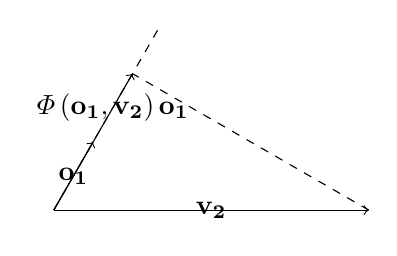
\begin{tikzpicture}[auto]
    \draw[->] (0,0)--(0.5,0.8660);
    \draw[->] (0,0)--(1,1.7321);
    \draw[dashed] (0,0)--(1.3333,2.3094);
    \draw[->] (0,0)--(4,0);
    \draw[dashed] (4,0)--(1,1.7321);
    \node (21) at (0.25,0.4330) {$\bf{o}_1 $};
    \node (31) at (0.75,1.2990) {$\varPhi \left( \bf{o}_1 ,\bf{v}_2 \right) \bf{o}_1 $};
    \node (12) at (2,0) {$\bf{v}_2 $};
    \end{tikzpicture}
    \qquad
    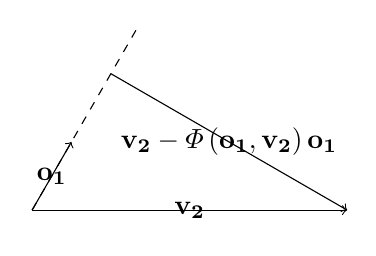
\begin{tikzpicture}[auto]
    \draw[->] (0,0)--(0.5,0.8660);
    \draw[dashed] (0,0)--(1.3333,2.3094);
    \draw[->] (0,0)--(4,0);
    \draw[->] (1,1.7321)--(4,0);
    \node (21) at (0.25,0.4330) {$\bf{o}_1 $};
    \node (31) at (2.5,0.8660) {$\bf{v}_2 -\varPhi \left( \bf{o}_1 ,\bf{v}_2 \right) \bf{o}_1 $};
    \node (12) at (2,0) {$\bf{v}_2 $};
    \end{tikzpicture}
    \vskip \baselineskip 
    \begin{tikzpicture}[auto]
    \draw[->] (0,0)--(0.5,0.8660);
    \draw[dashed] (0,0)--(1.3333,2.3094);
    \draw[->] (0,0)--(4,0);
    \draw[dashed] (1,1.7321)--(4,0);
    \draw[->] (0,0)--(3,-1.7321);
    \draw[dashed] (3,-1.7321)--(4,0);
    \node (21) at (0.25,0.4330) {$\bf{o}_1 $};
    \node (32) at (1.5,-0.8660) {$\bf{o}_2'$};
    \node (12) at (2,0) {$\bf{v}_2 $};
    \end{tikzpicture}
    \qquad
    \begin{tikzpicture}[auto]
    \draw[->] (0,0)--(0.5,0.8660);
    \draw[->] (0,0)--(0.8660,-0.5);
    \draw[dashed] (0,0)--(1.3333,2.3094);
    \draw[dashed] (0,0)--(4,0);
    \draw[dashed] (1,1.7321)--(4,0);
    \draw[dashed] (0,0)--(3,-1.7321);
    \draw[dashed] (3,-1.7321)--(4,0);
    \node (21) at (0.25,0.4330) {$\bf{o}_1 $};
    \node (32) at (0.4330,-0.25) {$\bf{o}_2 $};
    \end{tikzpicture}
\end{center}
\begin{proof}
$K \subseteq \mathbb{C}$なる体$K$上の$n$次元vector空間$V$上の内積空間$(V,\varPhi)$から誘導されるnorm空間$\left( V,\varphi_{\varPhi} \right)$、そのvector空間$V$の任意の基底$\left\langle \mathbf{v}_{i} \right\rangle_{i \in \varLambda_{n}}$が与えられたとき、$\forall i \in \varLambda_{n}$に対し、次のようにvector$\mathbf{o}_{i}$がおかれると、
\begin{align*}
\mathbf{o}_{i} = \frac{\mathbf{v}_{i} - \sum_{j \in \varLambda_{i - 1}} {\varPhi\left( \mathbf{o}_{j},\mathbf{v}_{i} \right)\mathbf{o}_{j}}}{\varphi_{\varPhi}\left( \mathbf{v}_{i} - \sum_{j \in \varLambda_{i - 1}} {\varPhi\left( \mathbf{o}_{j},\mathbf{v}_{i} \right)\mathbf{o}_{j}} \right)}
\end{align*}
$n = 1$のときでは明らかなので、$2 \leq n = l$のとき、その組$\left\langle \mathbf{o}_{i} \right\rangle_{i \in \varLambda_{l}}$はその部分空間$\mathrm{span}\left\{ \mathbf{v}_{i} \right\}_{i \in \varLambda_{l}}$上の基底をなし、さらに、$\forall k \in \varLambda_{l}$に対し、次式が成り立つと仮定しよう。
\begin{align*}
\mathrm{span}\left\{ \mathbf{v}_{i} \right\}_{i \in \varLambda_{k}} = \mathrm{span}\left\{ \mathbf{o}_{i} \right\}_{i \in \varLambda_{k}}
\end{align*}\par
$n = l + 1$のとき、次のようにおかれると、
\begin{align*}
\mathbf{o}_{l + 1}' = \mathbf{v}_{l + 1} - \sum_{j \in \varLambda_{l}} {\varPhi\left( \mathbf{o}_{j},\mathbf{v}_{l + 1} \right)\mathbf{o}_{j}}
\end{align*}
次のようになるかつ、
\begin{align*}
\mathbf{o}_{l + 1}' &= \mathbf{v}_{l + 1} - \sum_{j \in \varLambda_{l}} {\varPhi\left( \mathbf{o}_{j},\mathbf{v}_{l + 1} \right)\mathbf{o}_{j}}\\
&= - \sum_{j \in \varLambda_{l}} {\varPhi\left( \mathbf{o}_{j},\mathbf{v}_{l + 1} \right)\mathbf{o}_{j}} + \mathbf{v}_{l + 1}
\end{align*}
次のようになるので、
\begin{align*}
\mathbf{v}_{l + 1} &= \mathbf{v}_{l + 1} - \sum_{j \in \varLambda_{l}} {\varPhi\left( \mathbf{o}_{j},\mathbf{v}_{l + 1} \right)\mathbf{o}_{j}} + \sum_{j \in \varLambda_{l}} {\varPhi\left( \mathbf{o}_{j},\mathbf{v}_{l + 1} \right)\mathbf{o}_{j}}\\
&= \sum_{j \in \varLambda_{l}} {\varPhi\left( \mathbf{o}_{j},\mathbf{v}_{l + 1} \right)\mathbf{o}_{j}} + \mathbf{o}_{l + 1}'
\end{align*}
次式が成り立つ。
\begin{align*}
\mathbf{o}_{l + 1}' \in \mathrm{span}{\left\{ \mathbf{o}_{j} \right\}_{j \in \varLambda_{l}} \cup \left\{ \mathbf{v}_{l + 1} \right\}},\ \ \mathbf{v}_{l + 1} \in \mathrm{span}{\left\{ \mathbf{o}_{j} \right\}_{j \in \varLambda_{l}} \cup \left\{ \mathbf{o}_{l + 1}' \right\}}
\end{align*}
これにより、$\forall\mathbf{v} \in V$に対し、$\mathbf{v} \in \mathrm{span}{\left\{ \mathbf{o}_{j} \right\}_{j \in \varLambda_{l}} \cup \left\{ \mathbf{v}_{l + 1} \right\}}$が成り立つなら、次のように表されることができるので、
\begin{align*}
\mathbf{v} = \sum_{j \in \varLambda_{l}} {a_{j}\mathbf{o}_{j}} + a_{l + 1}\mathbf{v}_{l + 1},\ \ \mathbf{v}_{l + 1} = \sum_{j \in \varLambda_{l}} {b_{j}\mathbf{o}_{j}} + b_{l + 1}\mathbf{o}_{l + 1}'
\end{align*}
次のようになり、
\begin{align*}
\mathbf{v} &= \sum_{j \in \varLambda_{l}} {a_{j}\mathbf{o}_{j}} + a_{l + 1}\mathbf{v}_{l + 1}\\
&= \sum_{j \in \varLambda_{l}} {a_{j}\mathbf{o}_{j}} + a_{l + 1}\left( \sum_{j \in \varLambda_{l}} {b_{j}\mathbf{o}_{j}} + b_{l + 1}\mathbf{o}_{l + 1}' \right)\\
&= \sum_{j \in \varLambda_{l}} {a_{j}\mathbf{o}_{j}} + \sum_{j \in \varLambda_{l}} {a_{l + 1}b_{j}\mathbf{o}_{j}} + a_{l + 1}b_{l + 1}\mathbf{o}_{l + 1}'\\
&= \sum_{j \in \varLambda_{l}} {\left( a_{j} + a_{l + 1}b_{j} \right)\mathbf{o}_{j}} + a_{l + 1}b_{l + 1}\mathbf{o}_{l + 1}'
\end{align*}
したがって、$\mathbf{v} \in \mathrm{span}{\left\{ \mathbf{o}_{j} \right\}_{j \in \varLambda_{l}} \cup \left\{ \mathbf{o}_{l + 1}' \right\}}$が得られるかつ、$\mathbf{v} \in \mathrm{span}{\left\{ \mathbf{o}_{j} \right\}_{j \in \varLambda_{l}} \cup \left\{ \mathbf{o}_{l + 1}' \right\}}$が成り立つなら、次のように表されることができるので、
\begin{align*}
\mathbf{v} = \sum_{j \in \varLambda_{l}} {a_{j}\mathbf{o}_{j}} + a_{l + 1}\mathbf{o}_{l + 1}',\ \ \mathbf{o}_{l + 1}' = \sum_{j \in \varLambda_{l}} {b_{j}\mathbf{o}_{j}} + b_{l + 1}\mathbf{v}_{l + 1}
\end{align*}
次のようになり、
\begin{align*}
\mathbf{v} &= \sum_{j \in \varLambda_{l}} {a_{j}\mathbf{o}_{j}} + a_{l + 1}\mathbf{o}_{l + 1}'\\
&= \sum_{j \in \varLambda_{l}} {a_{j}\mathbf{o}_{j}} + a_{l + 1}\left( \sum_{j \in \varLambda_{l}} {b_{j}\mathbf{o}_{j}} + b_{l + 1}\mathbf{v}_{l + 1} \right)\\
&= \sum_{j \in \varLambda_{l}} {a_{j}\mathbf{o}_{j}} + \sum_{j \in \varLambda_{l}} {a_{l + 1}b_{j}\mathbf{o}_{j}} + a_{l + 1}b_{l + 1}\mathbf{v}_{l + 1}\\
&= \sum_{j \in \varLambda_{l}} {\left( a_{j} + a_{l + 1}b_{j} \right)\mathbf{o}_{j}} + a_{l + 1}b_{l + 1}\mathbf{v}_{l + 1}
\end{align*}
したがって、$\mathbf{v} \in \mathrm{span}{\left\{ \mathbf{o}_{j} \right\}_{j \in \varLambda_{l}} \cup \left\{ \mathbf{v}_{l + 1} \right\}}$が得られる。これにより、次式が成り立つ。
\begin{align*}
\mathrm{span}{\left\{ \mathbf{o}_{j} \right\}_{j \in \varLambda_{l}} \cup \left\{ \mathbf{v}_{l + 1} \right\}} = \mathrm{span}{\left\{ \mathbf{o}_{j} \right\}_{j \in \varLambda_{l}} \cup \left\{ \mathbf{o}_{l + 1}' \right\}}
\end{align*}\par
さらに、$\sum_{j \in \varLambda_{l}} {c_{j}\mathbf{o}_{j}} + c_{l + 1}\mathbf{o}_{l + 1}' = \mathbf{0}$が成り立つなら、数学的帰納法の仮定より$\mathrm{span}\left\{ \mathbf{v}_{i} \right\}_{i \in \varLambda_{l}} = \mathrm{span}\left\{ \mathbf{o}_{i} \right\}_{i \in \varLambda_{l}}$が成り立つので、$\forall j \in \varLambda_{l}$に対し、$o_{l + 1,j} = 0$とおくと、次のように表されることができるので、
\begin{align*}
\mathbf{o}_{j} = \sum_{i \in \varLambda_{l + 1}} {o_{ij}\mathbf{v}_{i}},\ \ \mathbf{o}_{l + 1}' = \sum_{i \in \varLambda_{l + 1}} {o_{i,l + 1}\mathbf{v}_{i}}
\end{align*}
次のようになり、
\begin{align*}
\mathbf{0} &= \sum_{j \in \varLambda_{l}} {c_{j}\mathbf{o}_{j}} + c_{l + 1}\mathbf{o}_{l + 1}'\\
&= \sum_{j \in \varLambda_{l}} {c_{j}\sum_{i \in \varLambda_{l + 1}} {o_{ij}\mathbf{v}_{i}}} + c_{l + 1}\sum_{i \in \varLambda_{l + 1}} {o_{i,l + 1}\mathbf{v}_{i}}\\
&= \sum_{i \in \varLambda_{l + 1}} {\sum_{j \in \varLambda_{l}} {c_{j}o_{ij}\mathbf{v}_{i}}} + \sum_{i \in \varLambda_{l + 1}} {c_{l + 1}o_{i,l + 1}\mathbf{v}_{i}}\\
&= \sum_{i \in \varLambda_{l + 1}} {\sum_{j \in \varLambda_{l + 1}} {c_{j}o_{ij}\mathbf{v}_{i}}}
\end{align*}
これらのvectors$\mathbf{v}_{i}$は線形独立であるので、$\forall i \in \varLambda_{l + 1}$に対し、$\sum_{j \in \varLambda_{l + 1}} {c_{j}o_{ij}} = 0$が成り立つ。これにより、次のようになる。
\begin{align*}
\left\{ \begin{matrix}
\sum_{j \in \varLambda_{l + 1}} {c_{j}o_{1j}} = 0 \\
\sum_{j \in \varLambda_{l + 1}} {c_{j}o_{2j}} = 0 \\
 \vdots \\
\sum_{j \in \varLambda_{l + 1}} {c_{j}o_{lj}} = 0 \\
\sum_{j \in \varLambda_{l + 1}} {c_{j}o_{l + 1,j}} = 0 \\
\end{matrix} \right.\  &\Leftrightarrow \left\{ \begin{matrix}
c_{1}o_{11} + c_{2}o_{12} + \cdots + c_{l}o_{1l} + c_{l + 1}o_{1,l + 1} = 0 \\
c_{1}o_{21} + c_{2}o_{22} + \cdots + c_{l}o_{2l} + c_{l + 1}o_{2,l + 1} = 0 \\
 \vdots \\
c_{1}o_{l1} + c_{2}o_{l2} + \cdots + c_{l}o_{ll} + c_{l + 1}o_{l,l + 1} = 0 \\
c_{1}o_{l + 1,1} + c_{2}o_{l + 1,2} + \cdots + c_{l}o_{l + 1,1} + c_{l + 1}o_{l + 1,l + 1} = 0 \\
\end{matrix} \right.\ \\
&\Leftrightarrow \begin{pmatrix}
c_{1}o_{11} + c_{2}o_{12} + \cdots + c_{l}o_{1l} + c_{l + 1}o_{1,l + 1} \\
c_{1}o_{21} + c_{2}o_{22} + \cdots + c_{l}o_{2l} + c_{l + 1}o_{2,l + 1} \\
 \vdots \\
c_{1}o_{l1} + c_{2}o_{l2} + \cdots + c_{l}o_{ll} + c_{l + 1}o_{l,l + 1} \\
c_{1}o_{l + 1,1} + c_{2}o_{l + 1,2} + \cdots + c_{l}o_{l + 1,1} + c_{l + 1}o_{l + 1,l + 1} \\
\end{pmatrix} = \begin{pmatrix}
0 \\
0 \\
 \vdots \\
0 \\
0 \\
\end{pmatrix}\\
&\Leftrightarrow \begin{pmatrix}
o_{11} & o_{12} & \cdots & o_{1l} & o_{1,l + 1} \\
o_{21} & o_{22} & \cdots & o_{2l} & o_{2,l + 1} \\
 \vdots & \vdots & \ddots & \vdots & \vdots \\
o_{l1} & o_{l2} & \cdots & o_{ll} & o_{l,l + 1} \\
o_{l + 1,1} & o_{l + 1,2} & \cdots & o_{l + 1,l} & o_{l + 1,l + 1} \\
\end{pmatrix}\begin{pmatrix}
c_{1} \\
c_{2} \\
 \vdots \\
c_{l} \\
c_{l + 1} \\
\end{pmatrix} = \begin{pmatrix}
0 \\
0 \\
 \vdots \\
0 \\
0 \\
\end{pmatrix}\\
&\Leftrightarrow \begin{pmatrix}
o_{11} & o_{12} & \cdots & o_{1l} & 0 \\
o_{21} & o_{22} & \cdots & o_{2l} & 0 \\
 \vdots & \vdots & \ddots & \vdots & \vdots \\
o_{l1} & o_{l2} & \cdots & o_{ll} & 0 \\
o_{l + 1,1} & o_{l + 1,2} & \cdots & o_{l + 1,l} & o_{l + 1,l + 1} \\
\end{pmatrix}\begin{pmatrix}
c_{1} \\
c_{2} \\
 \vdots \\
c_{l} \\
c_{l + 1} \\
\end{pmatrix} = \begin{pmatrix}
0 \\
0 \\
 \vdots \\
0 \\
0 \\
\end{pmatrix}
\end{align*}
そこで、基底$\left\langle \mathbf{v}_{i} \right\rangle_{i \in \varLambda_{l}}$が$\alpha$とおかれると、$\forall j \in \varLambda_{l}$に対し、$f\left( \mathbf{v}_{j} \right) = \mathbf{o}_{j}$なる線形写像$f:\mathrm{span}\left\{ \mathbf{v}_{i} \right\}_{i \in \varLambda_{l}} \rightarrow \mathrm{span}\left\{ \mathbf{v}_{i} \right\}_{i \in \varLambda_{l}}$が考えられると、これは線形同型写像であり、基底変換における線形同型写像$\varphi_{\alpha}$を用いて線形写像$\varphi_{\alpha}^{- 1} \circ f \circ \varphi_{\alpha}:K^{l} \rightarrow K^{l}$が考えられれば、そのvector空間$K^{l}$の標準直交基底$\left\langle \mathbf{e}_{i} \right\rangle_{i \in \varLambda_{l}}$を用いて次のようになることから、
\begin{align*}
\varphi_{\alpha}^{- 1} \circ f \circ \varphi_{\alpha}\left( \mathbf{e}_{j} \right) &= \varphi_{\alpha}^{- 1}\left( f\left( \varphi_{\alpha}\left( \mathbf{e}_{j} \right) \right) \right)\\
&= \varphi_{\alpha}^{- 1}\left( f\left( \mathbf{v}_{j} \right) \right)\\
&= \varphi_{\alpha}^{- 1}\left( \mathbf{o}_{j} \right)\\
&= \varphi_{\alpha}^{- 1}\left( \sum_{i \in \varLambda_{l + 1}} {o_{ij}\mathbf{v}_{i}} \right)\\
&= \varphi_{\alpha}^{- 1}\left( \sum_{i \in \varLambda_{l}} {o_{ij}\mathbf{v}_{i}} + o_{l + 1,j}\mathbf{v}_{l + 1} \right)\\
&= \varphi_{\alpha}^{- 1}\left( \sum_{i \in \varLambda_{l}} {o_{ij}\mathbf{v}_{i}} \right)\\
&= \sum_{i \in \varLambda_{l}} {o_{ij}\varphi_{\alpha}^{- 1}\left( \mathbf{v}_{i} \right)}\\
&= \sum_{i \in \varLambda_{l}} {o_{ij}\mathbf{e}_{i}} = \begin{pmatrix}
o_{1j} \\
o_{2j} \\
 \vdots \\
o_{lj} \\
\end{pmatrix}
\end{align*}
その線形写像$f$のその基底$\alpha$に関する表現行列$[ f]_{\alpha}^{\alpha}$が次を満たす。
\begin{align*}
[ f]_{\alpha}^{\alpha} = \begin{pmatrix}
o_{11} & o_{12} & \cdots & o_{1l} \\
o_{21} & o_{22} & \cdots & o_{2l} \\
 \vdots & \vdots & \ddots & \vdots \\
o_{l1} & o_{l2} & \cdots & o_{ll} \\
\end{pmatrix}
\end{align*}
その線形写像$f$が線形同型写像となっているので、その行列$[ f]_{\alpha}^{\alpha}$は正則行列である。したがって、ある正則行列$P$が存在して、$P[ f]_{\alpha}^{\alpha} = I_{l}$が成り立つ。次のようにおかれると、
\begin{align*}
P = \begin{pmatrix}
p_{11} & p_{12} & \cdots & p_{1l} \\
p_{21} & p_{22} & \cdots & p_{2l} \\
 \vdots & \vdots & \ddots & \vdots \\
p_{l1} & p_{l2} & \cdots & p_{ll} \\
\end{pmatrix},\ \ \mathbf{c} = \begin{pmatrix}
o_{l + 1,1} & o_{l + 1,2} & \cdots & o_{l + 1,l} \\
\end{pmatrix},\ \ \mathbf{x} = \begin{pmatrix}
c_{1} \\
c_{2} \\
 \vdots \\
c_{l} \\
c_{l + 1} \\
\end{pmatrix}
\end{align*}
行列$\begin{pmatrix}
P & \  \\
\  & 1 \\
\end{pmatrix}$も正則行列となるので\footnote{逆行列が$\begin{pmatrix}
  P^{- 1} & \  \\
  \  & 1 \\
  \end{pmatrix}$と与えられることから分かる。}、次のようになる。
\begin{align*}
\left\{ \begin{matrix}
\sum_{j \in \varLambda_{l + 1}} {c_{j}o_{1j}} = 0 \\
\sum_{j \in \varLambda_{l + 1}} {c_{j}o_{2j}} = 0 \\
 \vdots \\
\sum_{j \in \varLambda_{l + 1}} {c_{j}o_{lj}} = 0 \\
\sum_{j \in \varLambda_{l + 1}} {c_{j}o_{l + 1,j}} = 0 \\
\end{matrix} \right. &\Leftrightarrow \begin{pmatrix}
o_{11} & o_{12} & \cdots & o_{1l} & 0 \\
o_{21} & o_{22} & \cdots & o_{2l} & 0 \\
 \vdots & \vdots & \ddots & \vdots & \vdots \\
o_{l1} & o_{l2} & \cdots & o_{ll} & 0 \\
o_{l + 1,1} & o_{l + 1,2} & \cdots & o_{l + 1,l} & o_{l + 1,l + 1} \\
\end{pmatrix}\begin{pmatrix}
c_{1} \\
c_{2} \\
 \vdots \\
c_{l} \\
c_{l + 1} \\
\end{pmatrix} = \begin{pmatrix}
0 \\
0 \\
 \vdots \\
0 \\
0 \\
\end{pmatrix}\\
&\Leftrightarrow \begin{pmatrix}
[ f]_{\alpha}^{\alpha} & \  \\
\mathbf{c} & o_{l + 1,l + 1} \\
\end{pmatrix}\mathbf{x} = \mathbf{0}\\
&\Leftrightarrow \begin{pmatrix}
P & \  \\
\  & 1 \\
\end{pmatrix}\begin{pmatrix}
[ f]_{\alpha}^{\alpha} & \  \\
\mathbf{c} & o_{l + 1,l + 1} \\
\end{pmatrix}\mathbf{x} = \mathbf{0}\\
&\Leftrightarrow \begin{pmatrix}
P[ f]_{\alpha}^{\alpha} & \  \\
\mathbf{c} & o_{l + 1,l + 1} \\
\end{pmatrix}\mathbf{x} = \mathbf{0}\\
&\Leftrightarrow \begin{pmatrix}
I_{l} & \  \\
\mathbf{c} & o_{l + 1,l + 1} \\
\end{pmatrix}\mathbf{x} = \mathbf{0}
\end{align*}
そこで、行の基本変形により$\begin{pmatrix}
I_{l} & \  \\
\mathbf{c} & o_{l + 1,l + 1} \\
\end{pmatrix} \rightarrow \begin{pmatrix}
I_{l} & \  \\
\mathbf{\ } & o_{l + 1,l + 1} \\
\end{pmatrix}$とすることができるので、そうすれば、次のようになる。
\begin{align*}
\left\{ \begin{matrix}
\sum_{j \in \varLambda_{l + 1}} {c_{j}o_{1j}} = 0 \\
\sum_{j \in \varLambda_{l + 1}} {c_{j}o_{2j}} = 0 \\
 \vdots \\
\sum_{j \in \varLambda_{l + 1}} {c_{j}o_{lj}} = 0 \\
\sum_{j \in \varLambda_{l + 1}} {c_{j}o_{l + 1,j}} = 0 \\
\end{matrix} \right. &\Leftrightarrow \begin{pmatrix}
I_{l} & \  \\
\mathbf{c} & o_{l + 1,l + 1} \\
\end{pmatrix}\mathbf{x} = \mathbf{0}\\
&\Leftrightarrow \begin{pmatrix}
I_{l} & \  \\
\mathbf{\ } & o_{l + 1,l + 1} \\
\end{pmatrix}\mathbf{x} = \mathbf{0}
\end{align*}\par
ここで、$o_{l + 1,l + 1} = 0$と仮定すると、$\mathbf{o}_{l + 1}' = \sum_{i \in \varLambda_{l + 1}} {o_{i,l + 1}\mathbf{v}_{i}} = \sum_{i \in \varLambda_{l}} {o_{i,l + 1}\mathbf{v}_{i}}$より$\mathbf{o}_{l + 1}' = \mathrm{span}\left\{ \mathbf{o}_{j} \right\}_{j \in \varLambda_{l}}$が得られる。そこで、$\mathbf{v}_{l + 1} \in \mathrm{span}{\left\{ \mathbf{o}_{j} \right\}_{j \in \varLambda_{l}} \cup \left\{ \mathbf{o}_{l + 1}' \right\}}$が成り立つかつ、数学的帰納法の仮定より$\mathrm{span}\left\{ \mathbf{v}_{i} \right\}_{i \in \varLambda_{l}} = \mathrm{span}\left\{ \mathbf{o}_{j} \right\}_{j \in \varLambda_{l}}$が成り立つので、$\mathbf{v}_{l + 1} \in \mathrm{span}\left\{ \mathbf{v}_{i} \right\}_{i \in \varLambda_{l}}$となってそのvector$\mathbf{v}_{l + 1}$は$i \in \varLambda_{l}$なるそれらのvectors$\mathbf{v}_{i}$の線形結合であり、したがって、$i \in \varLambda_{l + 1}$なるこれらのvectors$\mathbf{v}_{i}$は線形従属となるが、これはこれらのvectors$\mathbf{v}_{i}$がそのvector空間$V$の基底をなすことに矛盾している。\par
したがって、$o_{l + 1,l + 1} \neq 0$が成り立ち行の基本変形により次のようになるので、
\begin{align*}
\begin{pmatrix}
I_{l} & \  \\
\mathbf{\ } & o_{l + 1,l + 1} \\
\end{pmatrix} \rightarrow \begin{pmatrix}
I_{l} & \  \\
\mathbf{\ } & 1 \\
\end{pmatrix} = I_{l + 1}
\end{align*}
次のようになり、
\begin{align*}
\left\{ \begin{matrix}
\sum_{j \in \varLambda_{l + 1}} {c_{j}o_{1j}} = 0 \\
\sum_{j \in \varLambda_{l + 1}} {c_{j}o_{2j}} = 0 \\
 \vdots \\
\sum_{j \in \varLambda_{l + 1}} {c_{j}o_{lj}} = 0 \\
\sum_{j \in \varLambda_{l + 1}} {c_{j}o_{l + 1,j}} = 0 \\
\end{matrix} \right. &\Leftrightarrow \begin{pmatrix}
I_{l} & \  \\
\mathbf{\ } & o_{l + 1,l + 1} \\
\end{pmatrix}\mathbf{x} = \mathbf{0}\\
&\Leftrightarrow I_{l + 1}\mathbf{x} = \mathbf{x} = \mathbf{0}
\end{align*}
したがって、$\begin{pmatrix}
c_{1} \\
c_{2} \\
 \vdots \\
c_{l} \\
c_{l + 1} \\
\end{pmatrix} = \begin{pmatrix}
0 \\
0 \\
 \vdots \\
0 \\
0 \\
\end{pmatrix}$が得られる。これにより、$i \in \varLambda_{l}$なるそれらのvectors$\mathbf{o}_{i}$、$\mathbf{o}_{l + 1}'$は線形独立である。\par
したがって、$\mathbf{o}_{l + 1}' \neq \mathbf{0}$が成り立つので、$\varphi_{\varPhi}\left( \mathbf{o}_{l + 1}' \right) \neq 0$が得られる。そこで、$\mathbf{o}_{l + 1} = \frac{\mathbf{o}_{l + 1}'}{\varphi_{\varPhi}\left( \mathbf{o}_{l + 1}' \right)}$とおかれれば、もちろん、$\forall i \in \varLambda_{l + 1}$に対し、それらのvectors$\mathbf{o}_{i}$は線形独立であり、さらに、次のようになることから、
\begin{align*}
\mathrm{span}\left\{ \mathbf{v}_{i} \right\}_{i \in \varLambda_{l + 1}} &= \mathrm{span}\left\{ \mathbf{v}_{i} \right\}_{i \in \varLambda_{l}} \oplus \mathrm{span}\left\{ \mathbf{v}_{l + 1} \right\}\\
&= \mathrm{span}\left\{ \mathbf{o}_{j} \right\}_{j \in \varLambda_{l}} \oplus \mathrm{span}\left\{ \mathbf{v}_{l + 1} \right\}\\
&= \mathrm{span}{\left\{ \mathbf{o}_{j} \right\}_{j \in \varLambda_{l}} \cup \left\{ \mathbf{v}_{l + 1} \right\}}\\
&= \mathrm{span}{\left\{ \mathbf{o}_{j} \right\}_{j \in \varLambda_{l}} \cup \left\{ \mathbf{o}_{l + 1}' \right\}}\\
&= \mathrm{span}\left\{ \mathbf{o}_{j} \right\}_{j \in \varLambda_{l}} \oplus \mathrm{span}\left\{ \mathbf{o}_{l + 1}' \right\}\\
&= \mathrm{span}\left\{ \mathbf{o}_{j} \right\}_{j \in \varLambda_{l}} \oplus \mathrm{span}\left\{ \mathbf{o}_{l + 1} \right\}\\
&= \mathrm{span}{\left\{ \mathbf{o}_{j} \right\}_{j \in \varLambda_{l}} \cup \left\{ \mathbf{o}_{l + 1} \right\}}\\
&= \mathrm{span}\left\{ \mathbf{o}_{j} \right\}_{j \in \varLambda_{l + 1}}
\end{align*}
$j \in \varLambda_{l + 1}$なるこれらのvectors$\mathbf{o}_{j}$はその部分空間$\mathrm{span}\left\{ \mathbf{v}_{i} \right\}_{i \in \varLambda_{l + 1}}$を生成する。以上の議論により、その組$\left\langle \mathbf{o}_{j} \right\rangle_{j \in \varLambda_{l + 1}}$はその部分空間$\mathrm{span}\left\{ \mathbf{v}_{i} \right\}_{i \in \varLambda_{l + 1}}$の基底をなす。\par
また、$\forall i,j \in \varLambda_{l + 1}$に対し、次のようになることから、
\begin{align*}
i,j \in \varLambda_{l + 1} &\Leftrightarrow i \in \varLambda_{l + 1} \land j \in \varLambda_{l + 1}\\
&\Leftrightarrow \left( i \in \varLambda_{l} \vee i = l + 1 \right) \land \left( j \in \varLambda_{l} \vee j = l + 1 \right)\\
&\Leftrightarrow \left( i \in \varLambda_{l} \land j \in \varLambda_{l} \right) \vee \left( i \in \varLambda_{l} \land j = l + 1 \right) \vee \left( i = l + 1 \land j \in \varLambda_{l} \right) \vee (i = l + 1 \land j = l + 1)\\
&\Leftrightarrow i,j \in \varLambda_{l} \vee \left( i \in \varLambda_{l} \land j = l + 1 \right) \vee \left( i = l + 1 \land j \in \varLambda_{l} \right) \vee i = j = l + 1
\end{align*}
$i = j$のとき、$i \in \varLambda_{l}$かつ$j = l + 1$、あるいは、$i = l + 1$かつ$j \in \varLambda_{l}$が成り立つことはない。$i,j \in \varLambda_{l}$のとき、数学的帰納法の仮定により、$\varPhi\left( \mathbf{o}_{i},\mathbf{o}_{j} \right) = 1$が成り立っている。$i = j = l + 1$のとき、次のようになる。
\begin{align*}
\varPhi\left( \mathbf{o}_{i},\mathbf{o}_{j} \right) &= \varPhi\left( \mathbf{o}_{l + 1},\mathbf{o}_{l + 1} \right)\\
&= \varPhi\left( \frac{\mathbf{o}_{l + 1}'}{\varphi_{\varPhi}\left( \mathbf{o}_{l + 1}' \right)},\frac{\mathbf{o}_{l + 1}'}{\varphi_{\varPhi}\left( \mathbf{o}_{l + 1}' \right)} \right)\\
&= \frac{1}{{\varphi_{\varPhi}\left( \mathbf{o}_{l + 1}' \right)}^{2}}\varPhi\left( \mathbf{o}_{l + 1}',\mathbf{o}_{l + 1}' \right)\\
&= \frac{1}{{\varphi_{\varPhi}\left( \mathbf{o}_{l + 1}' \right)}^{2}}{\varphi_{\varPhi}\left( \mathbf{o}_{l + 1}' \right)}^{2} = 1
\end{align*}
$i \neq j$のとき、$i,j \in \varLambda_{l}$のとき、数学的帰納法の仮定により、$\varPhi\left( \mathbf{o}_{i},\mathbf{o}_{j} \right) = 0$が成り立っている。$i \in \varLambda_{l}$かつ$j = l + 1$のとき、次のようになる。
\begin{align*}
\varPhi\left( \mathbf{o}_{i},\mathbf{o}_{j} \right) &= \varPhi\left( \mathbf{o}_{i},\mathbf{o}_{l + 1} \right)\\
&= \varPhi\left( \mathbf{o}_{i},\frac{\mathbf{o}_{l + 1}'}{\varphi_{\varPhi}\left( \mathbf{o}_{l + 1}' \right)} \right)\\
&= \frac{1}{\varphi_{\varPhi}\left( \mathbf{o}_{l + 1}' \right)}\varPhi\left( \mathbf{o}_{i},\mathbf{o}_{l + 1}' \right)\\
&= \frac{1}{\varphi_{\varPhi}\left( \mathbf{o}_{l + 1}' \right)}\varPhi\left( \mathbf{o}_{i},\mathbf{v}_{l + 1} - \sum_{j \in \varLambda_{l}} {\varPhi\left( \mathbf{o}_{j},\mathbf{v}_{l + 1} \right)\mathbf{o}_{j}} \right)\\
&= \frac{1}{\varphi_{\varPhi}\left( \mathbf{o}_{l + 1}' \right)}\left( \varPhi\left( \mathbf{o}_{i},\mathbf{v}_{l + 1} \right) - \sum_{j \in \varLambda_{l}} {\varPhi\left( \mathbf{o}_{j},\mathbf{v}_{l + 1} \right)\varPhi\left( \mathbf{o}_{i},\mathbf{o}_{j} \right)} \right)\\
&= \frac{1}{\varphi_{\varPhi}\left( \mathbf{o}_{l + 1}' \right)}\left( \varPhi\left( \mathbf{o}_{i},\mathbf{v}_{l + 1} \right) - \sum_{\scriptsize \begin{matrix} j \in \varLambda_{l}\\i \neq j\\\end{matrix}} {\varPhi\left( \mathbf{o}_{j},\mathbf{v}_{l + 1} \right)\varPhi\left( \mathbf{o}_{i},\mathbf{o}_{j} \right)} - \varPhi\left( \mathbf{o}_{i},\mathbf{v}_{l + 1} \right)\varPhi\left( \mathbf{o}_{i},\mathbf{o}_{i} \right) \right)\\
&= \frac{1}{\varphi_{\varPhi}\left( \mathbf{o}_{l + 1}' \right)}\left( \varPhi\left( \mathbf{o}_{i},\mathbf{v}_{l + 1} \right) - \sum_{\scriptsize \begin{matrix} j \in \varLambda_{l}\\i \neq j\\\end{matrix}} {\varPhi\left( \mathbf{o}_{j},\mathbf{v}_{l + 1} \right) \cdot 0} - \varPhi\left( \mathbf{o}_{i},\mathbf{v}_{l + 1} \right) \cdot 1 \right)\\
&= \frac{1}{\varphi_{\varPhi}\left( \mathbf{o}_{l + 1}' \right)}\left( \varPhi\left( \mathbf{o}_{i},\mathbf{v}_{l + 1} \right) - \varPhi\left( \mathbf{o}_{i},\mathbf{v}_{l + 1} \right) \right) = 0
\end{align*}
$i = l + 1$かつ$j \in \varLambda_{l}$のときも同様にして示される。これにより、その組$\left\langle \mathbf{o}_{i} \right\rangle_{i \in \varLambda_{l + 1}}$はその部分空間$\mathrm{span}\left\{ \mathbf{v}_{i} \right\}_{i \in \varLambda_{l + 1}}$上の直交基底をなしている。\par
さらに、$\forall i \in \varLambda_{l + 1}$に対し、$i \in \varLambda_{l}$のとき、数学的帰納法の仮定より$\varphi_{\varPhi}\left( \mathbf{o}_{i} \right) = 1$が成り立つ。$i = l + 1$のとき、定義より次のようになる。
\begin{align*}
\varphi_{\varPhi}\left( \mathbf{o}_{l + 1} \right) &= \varphi_{\varPhi}\left( \frac{\mathbf{o}_{l + 1}'}{\varphi_{\varPhi}\left( \mathbf{o}_{l + 1}' \right)} \right)\\
&= \frac{1}{\varphi_{\varPhi}\left( \mathbf{o}_{l + 1}' \right)}\varphi_{\varPhi}\left( \mathbf{o}_{l + 1}' \right) = 1
\end{align*}
これにより、その組$\left\langle \mathbf{o}_{i} \right\rangle_{i \in \varLambda_{l + 1}}$はその部分空間$\mathrm{span}\left\{ \mathbf{v}_{i} \right\}_{i \in \varLambda_{l + 1}}$上の正規直交基底をなしている。\par
以上、数学的帰納法により、$\forall k \in \varLambda_{n}$に対し、その組$\left\langle \mathbf{o}_{i} \right\rangle_{i \in \varLambda_{k}}$はその部分空間$\mathrm{span}\left\{ \mathbf{v}_{i} \right\}_{i \in \varLambda_{k}}$上の正規直交基底をなし、さらに、次式が成り立つ。
\begin{align*}
\mathrm{span}\left\{ \mathbf{v}_{i} \right\}_{i \in \varLambda_{k}} = \mathrm{span}\left\{ \mathbf{o}_{i} \right\}_{i \in \varLambda_{k}}
\end{align*}
特に、$V = \mathrm{span}\left\{ \mathbf{v}_{i} \right\}_{i \in \varLambda_{n}}$が成り立つので、その組$\left\langle \mathbf{o}_{i} \right\rangle_{i \in \varLambda_{n}}$はそのvector空間$V$上の正規直交基底をなす。さらに、$\forall k \in \varLambda_{n}$に対し、次式が成り立つ。
\begin{align*}
\mathrm{span}\left\{ \mathbf{v}_{i} \right\}_{i \in \varLambda_{k}} = \mathrm{span}\left\{ \mathbf{o}_{i} \right\}_{i \in \varLambda_{k}}
\end{align*}
\end{proof}\par
例えば、体$\mathbb{R}$上のvector空間$\mathrm{span}\begin{Bmatrix}
\begin{pmatrix}
1 \\
1 \\
0 \\
1 \\
\end{pmatrix} & \begin{pmatrix}
1 \\
2 \\
1 \\
1 \\
\end{pmatrix} & \begin{pmatrix}
0 \\
1 \\
0 \\
0 \\
\end{pmatrix} & \begin{pmatrix}
1 \\
2 \\
0 \\
1 \\
\end{pmatrix} \\
\end{Bmatrix}$の標準内積空間$\left( \mathbb{R}^{n},\left( \bullet \middle| \bullet \right) \right)$における正規直交基底をGram-Schmidtの正規直交化法で求めよう。まず、そのvector空間$\mathrm{span}\begin{Bmatrix}
\begin{pmatrix}
1 \\
1 \\
0 \\
1 \\
\end{pmatrix} & \begin{pmatrix}
1 \\
2 \\
1 \\
1 \\
\end{pmatrix} & \begin{pmatrix}
0 \\
1 \\
0 \\
0 \\
\end{pmatrix} & \begin{pmatrix}
1 \\
2 \\
0 \\
1 \\
\end{pmatrix} \\
\end{Bmatrix}$の基底を求めよう。このとき、次のようになることから、
\begin{align*}
\begin{pmatrix}
1 & 1 & 0 & 1 \\
1 & 2 & 1 & 2 \\
0 & 1 & 0 & 0 \\
1 & 1 & 0 & 1 \\
\end{pmatrix} \rightarrow \begin{pmatrix}
1 & 1 & 0 & 1 \\
0 & 1 & 1 & 1 \\
0 & 1 & 0 & 0 \\
0 & 0 & 0 & 0 \\
\end{pmatrix} \rightarrow \begin{pmatrix}
1 & 1 & 0 & 1 \\
0 & 1 & 0 & 0 \\
0 & 1 & 1 & 1 \\
0 & 0 & 0 & 0 \\
\end{pmatrix} \rightarrow \begin{pmatrix}
1 & 0 & 0 & 1 \\
0 & 1 & 0 & 0 \\
0 & 0 & 1 & 1 \\
0 & 0 & 0 & 0 \\
\end{pmatrix}
\end{align*}
定理\ref{2.1.8.9}よりそのvector空間$\mathrm{span}\begin{Bmatrix}
\begin{pmatrix}
1 \\
1 \\
0 \\
1 \\
\end{pmatrix} & \begin{pmatrix}
1 \\
2 \\
1 \\
1 \\
\end{pmatrix} & \begin{pmatrix}
0 \\
1 \\
0 \\
0 \\
\end{pmatrix} & \begin{pmatrix}
1 \\
2 \\
0 \\
1 \\
\end{pmatrix} \\
\end{Bmatrix}$の基底が$\left\langle \begin{matrix}
\begin{pmatrix}
1 \\
1 \\
0 \\
1 \\
\end{pmatrix} & \begin{pmatrix}
1 \\
2 \\
1 \\
1 \\
\end{pmatrix} & \begin{pmatrix}
0 \\
1 \\
0 \\
0 \\
\end{pmatrix} \\
\end{matrix} \right\rangle$と与えられる。これから、Gram-Schmidtの正規直交化法により、次のようになるので、
\begin{align*}
\mathbf{o}_{1}' &= \begin{pmatrix}
  1 \\
  1 \\
  0 \\
  1 \\
\end{pmatrix}\\
\mathbf{o}_{1} &= \frac{\mathbf{o}_{1}'}{\left\| \mathbf{o}_{1}' \right\|} = \frac{\begin{pmatrix}
  1 \\
  1 \\
  0 \\
  1 \\
\end{pmatrix}}{\left\| \begin{pmatrix}
  1 \\
  1 \\
  0 \\
  1 \\
\end{pmatrix} \right\|} = \frac{\begin{pmatrix}
  1 \\
  1 \\
  0 \\
  1 \\
\end{pmatrix}}{\sqrt{\left( \begin{pmatrix}
  1 \\
  1 \\
  0 \\
  1 \\
\end{pmatrix} \middle| \begin{pmatrix}
  1 \\
  1 \\
  0 \\
  1 \\
\end{pmatrix} \right)}}\\
&= \frac{\begin{pmatrix}
  1 \\
  1 \\
  0 \\
  1 \\
\end{pmatrix}}{\sqrt{\begin{matrix}
  \  & 1 \cdot 1 \\
   + & 1 \cdot 1 \\
   + & 0 \cdot 0 \\
   + & 1 \cdot 1 \\
\end{matrix}}} = {1}/{\sqrt{3}}\begin{pmatrix}
  1 \\
  1 \\
  0 \\
  1 \\
\end{pmatrix} = \begin{pmatrix}
  {1}/{\sqrt{3}} \\
  {1}/{\sqrt{3}} \\
  0 \\
  {1}/{\sqrt{3}} \\
\end{pmatrix}\\
\mathbf{o}_{2}' &= \begin{pmatrix}
  1 \\
  2 \\
  1 \\
  1 \\
\end{pmatrix} - \left( \begin{pmatrix}
  {1}/{\sqrt{3}} \\
  {1}/{\sqrt{3}} \\
  0 \\
  {1}/{\sqrt{3}} \\
\end{pmatrix} \middle| \begin{pmatrix}
  1 \\
  2 \\
  1 \\
  1 \\
\end{pmatrix} \right)\begin{pmatrix}
  {1}/{\sqrt{3}} \\
  {1}/{\sqrt{3}} \\
  0 \\
  {1}/{\sqrt{3}} \\
\end{pmatrix}\\
&= \begin{pmatrix}
  1 \\
  2 \\
  1 \\
  1 \\
\end{pmatrix} - \begin{pmatrix}
  \  & \left( {1}/{\sqrt{3}} \right) \cdot 1 \\
   + & \left( {1}/{\sqrt{3}} \right) \cdot 2 \\
   + & 0 \cdot 1 \\
   + & \left( {1}/{\sqrt{3}} \right) \cdot 1 \\
\end{pmatrix}\begin{pmatrix}
  {1}/{\sqrt{3}} \\
  {1}/{\sqrt{3}} \\
  0 \\
  {1}/{\sqrt{3}} \\
\end{pmatrix}\\
&= \begin{pmatrix}
  1 \\
  2 \\
  1 \\
  1 \\
\end{pmatrix} - {4}/{\sqrt{3}}\begin{pmatrix}
  {1}/{\sqrt{3}} \\
  {1}/{\sqrt{3}} \\
  0 \\
  {1}/{\sqrt{3}} \\
\end{pmatrix} = \begin{pmatrix}
  1 \\
  2 \\
  1 \\
  1 \\
\end{pmatrix} - \begin{pmatrix}
  {4}/{3} \\
  {4}/{3} \\
  0 \\
  {4}/{3} \\
\end{pmatrix} = \begin{pmatrix}
   - {1}/{3} \\
  {2}/{3} \\
  1 \\
   - {1}/{3} \\
\end{pmatrix}\\
\mathbf{o}_{2} &= \frac{\mathbf{o}_{2}'}{\left\| \mathbf{o}_{2}' \right\|} = \frac{\begin{pmatrix}
   - {1}/{3} \\
  {2}/{3} \\
  1 \\
   - {1}/{3} \\
\end{pmatrix}}{\left\| \begin{pmatrix}
   - {1}/{3} \\
  {2}/{3} \\
  1 \\
   - {1}/{3} \\
\end{pmatrix} \right\|} = \frac{\begin{pmatrix}
   - {1}/{3} \\
  {2}/{3} \\
  1 \\
   - {1}/{3} \\
\end{pmatrix}}{\sqrt{\left( \begin{pmatrix}
   - {1}/{3} \\
  {2}/{3} \\
  1 \\
   - {1}/{3} \\
\end{pmatrix} \middle| \begin{pmatrix}
   - {1}/{3} \\
  {2}/{3} \\
  1 \\
   - {1}/{3} \\
\end{pmatrix} \right)}}\\
&= \frac{\begin{pmatrix}
   - {1}/{3} \\
  {2}/{3} \\
  1 \\
   - {1}/{3} \\
\end{pmatrix}}{\sqrt{\begin{matrix}
  \  & \left( - {1}/{3} \right) \cdot \left( - {1}/{3} \right) \\
   + & \left( {2}/{3} \right) \cdot \left( {2}/{3} \right) \\
   + & 1 \cdot 1 \\
   + & \left( - {1}/{3} \right) \cdot \left( - {1}/{3} \right) \\
\end{matrix}}} = \sqrt{{3}/{5}}\begin{pmatrix}
   - {1}/{3} \\
  {2}/{3} \\
  1 \\
   - {1}/{3} \\
\end{pmatrix} = \begin{pmatrix}
   - {1}/{\sqrt{15}} \\
  {2}/{\sqrt{15}} \\
  {3}/{\sqrt{15}} \\
   - {1}/{\sqrt{15}} \\
\end{pmatrix}\\
\mathbf{o}_{3}' &= \begin{pmatrix}
  0 \\
  1 \\
  0 \\
  0 \\
\end{pmatrix} - \left( \begin{pmatrix}
  {1}/{\sqrt{3}} \\
  {1}/{\sqrt{3}} \\
  0 \\
  {1}/{\sqrt{3}} \\
\end{pmatrix} \middle| \begin{pmatrix}
  0 \\
  1 \\
  0 \\
  0 \\
\end{pmatrix} \right)\begin{pmatrix}
  {1}/{\sqrt{3}} \\
  {1}/{\sqrt{3}} \\
  0 \\
  {1}/{\sqrt{3}} \\
\end{pmatrix} - \left( \begin{pmatrix}
   - {1}/{\sqrt{15}} \\
  {2}/{\sqrt{15}} \\
  {\sqrt{3}}/{\sqrt{5}} \\
   - {1}/{\sqrt{15}} \\
\end{pmatrix} \middle| \begin{pmatrix}
  0 \\
  1 \\
  0 \\
  0 \\
\end{pmatrix} \right)\begin{pmatrix}
   - {1}/{\sqrt{15}} \\
  {2}/{\sqrt{15}} \\
  {\sqrt{3}}/{\sqrt{5}} \\
   - {1}/{\sqrt{15}} \\
\end{pmatrix}\\
&= \begin{pmatrix}
  0 \\
  1 \\
  0 \\
  0 \\
\end{pmatrix} - \begin{pmatrix}
  \  & \left( {1}/{\sqrt{3}} \right) \cdot 0 \\
   + & \left( {1}/{\sqrt{3}} \right) \cdot 1 \\
   + & 0 \cdot 0 \\
   + & \left( {1}/{\sqrt{3}} \right) \cdot 0 \\
\end{pmatrix}\begin{pmatrix}
  {1}/{\sqrt{3}} \\
  {1}/{\sqrt{3}} \\
  0 \\
  {1}/{\sqrt{3}} \\
\end{pmatrix} - \begin{pmatrix}
  \left( - {1}/{\sqrt{15}} \right) \cdot 0 \\
   + \left( {2}/{\sqrt{15}} \right) \cdot 1 \\
   + \left( {\sqrt{3}}/{\sqrt{5}} \right) \cdot 0 \\
   + \left( - {1}/{\sqrt{15}} \right) \cdot 0 \\
\end{pmatrix}\begin{pmatrix}
   - {1}/{\sqrt{15}} \\
  {2}/{\sqrt{15}} \\
  {\sqrt{3}}/{\sqrt{5}} \\
   - {1}/{\sqrt{15}} \\
\end{pmatrix}\\
&= \begin{pmatrix}
  0 \\
  1 \\
  0 \\
  0 \\
\end{pmatrix} - {1}/{\sqrt{3}}\begin{pmatrix}
  {1}/{\sqrt{3}} \\
  {1}/{\sqrt{3}} \\
  0 \\
  {1}/{\sqrt{3}} \\
\end{pmatrix} - {2}/{\sqrt{15}}\begin{pmatrix}
   - {1}/{\sqrt{15}} \\
  {2}/{\sqrt{15}} \\
  {\sqrt{3}}/{\sqrt{5}} \\
   - {1}/{\sqrt{15}} \\
\end{pmatrix}\\
&= \begin{pmatrix}
  0 \\
  1 \\
  0 \\
  0 \\
\end{pmatrix} - \begin{pmatrix}
  {1}/{3} \\
  {1}/{3} \\
  0 \\
  {1}/{3} \\
\end{pmatrix} - \begin{pmatrix}
   - {2}/{15} \\
  {4}/{15} \\
  {2}/{5} \\
   - {2}/{15} \\
\end{pmatrix} = \begin{pmatrix}
   - {1}/{5} \\
  {2}/{5} \\
   - {2}/{5} \\
   - {1}/{5} \\
\end{pmatrix}\\
\mathbf{o}_{3} &= \frac{\mathbf{o}_{3}'}{\left\| \mathbf{o}_{3}' \right\|} = \frac{\begin{pmatrix}
   - {1}/{5} \\
  {2}/{5} \\
   - {2}/{5} \\
   - {1}/{5} \\
\end{pmatrix}}{\left\| \begin{pmatrix}
   - {1}/{5} \\
  {2}/{5} \\
   - {2}/{5} \\
   - {1}/{5} \\
\end{pmatrix} \right\|} = \frac{\begin{pmatrix}
   - {1}/{5} \\
  {2}/{5} \\
   - {2}/{5} \\
   - {1}/{5} \\
\end{pmatrix}}{\sqrt{\left( \begin{pmatrix}
   - {1}/{5} \\
  {2}/{5} \\
   - {2}/{5} \\
   - {1}/{5} \\
\end{pmatrix} \middle| \begin{pmatrix}
   - {1}/{5} \\
  {2}/{5} \\
   - {2}/{5} \\
   - {1}/{5} \\
\end{pmatrix} \right)}}\\
  &= \frac{\begin{pmatrix}
   - {1}/{5} \\
  {2}/{5} \\
   - {2}/{5} \\
   - {1}/{5} \\
\end{pmatrix}}{\sqrt{\begin{matrix}
  \  & \left( - {1}/{5} \right) \cdot \left( - {1}/{5} \right) \\
   + & \left( {2}/{5} \right) \cdot \left( {2}/{5} \right) \\
   + & \left( - {2}/{5} \right) \cdot \left( - {2}/{5} \right) \\
   + & \left( - {1}/{5} \right) \cdot \left( - {1}/{5} \right) \\
\end{matrix}}} = \sqrt{\frac{5}{2}}\begin{pmatrix}
   - {1}/{5} \\
  {2}/{5} \\
   - {2}/{5} \\
   - {1}/{5} \\
\end{pmatrix} = \begin{pmatrix}
   - {1}/{\sqrt{10}} \\
  {2}/{\sqrt{10}} \\
   - {2}/{\sqrt{10}} \\
   - {1}/{\sqrt{10}} \\
\end{pmatrix}
\end{align*}
求めるそのvector空間$\mathrm{span}\begin{Bmatrix}
\begin{pmatrix}
  1 \\
  1 \\
  0 \\
  1 \\
\end{pmatrix} & \begin{pmatrix}
  1 \\
  2 \\
  1 \\
  1 \\
\end{pmatrix} & \begin{pmatrix}
  0 \\
  1 \\
  0 \\
  0 \\
\end{pmatrix} & \begin{pmatrix}
  1 \\
  2 \\
  0 \\
  1 \\
\end{pmatrix} \\
\end{Bmatrix}$の正規直交基底が$\left\langle \begin{matrix}
\begin{pmatrix}
  {1}/{\sqrt{3}} \\
  {1}/{\sqrt{3}} \\
  0 \\
  {1}/{\sqrt{3}} \\
\end{pmatrix} & \begin{pmatrix}
   - {1}/{\sqrt{15}} \\
  {2}/{\sqrt{15}} \\
  {3}/{\sqrt{15}} \\
   - {1}/{\sqrt{15}} \\
\end{pmatrix} & \begin{pmatrix}
   - {1}/{\sqrt{10}} \\
  {2}/{\sqrt{10}} \\
   - {2}/{\sqrt{10}} \\
   - {1}/{\sqrt{10}} \\
\end{pmatrix} \\
\end{matrix} \right\rangle$と与えられる。
\begin{thm}\label{2.3.6.12}
$K \subseteq \mathbb{C}$なる体$K$上の$n$次元vector空間$V$上の内積空間$(V,\varPhi)$から誘導されるnorm空間$\left( V,\varphi_{\varPhi} \right)$、そのvector空間$V$の$r \leq n$なる正規直交系$\left\langle \mathbf{o}_{i} \right\rangle_{i \in \varLambda_{r}}$が与えられたとき、$i \in \varLambda_{n} \setminus \varLambda_{r}$なる適切な$n - r$つのvectors$\mathbf{o}_{i}$を付け加えた組$\left\langle \mathbf{o}_{i} \right\rangle_{i \in \varLambda_{n}}$がそのvector空間$V$の正規直交基底をなすようにすることができる。
\end{thm}
\begin{proof}
$K \subseteq \mathbb{C}$なる体$K$上の$n$次元vector空間$V$上の内積空間$(V,\varPhi)$から誘導されるnorm空間$\left( V,\varphi_{\varPhi} \right)$、そのvector空間$V$の$r \leq n$なる正規直交系$\left\langle \mathbf{o}_{i} \right\rangle_{i \in \varLambda_{r}}$が与えられたとき、定理\ref{2.3.6.10}よりそれらのvectors$\mathbf{o}_{i}$は線形独立であるので、その組$\left\langle \mathbf{o}_{i} \right\rangle_{i \in \varLambda_{r}}$はそれらのvectors$\mathbf{o}_{i}$から生成される部分空間$\mathrm{span}\left\{ \mathbf{o}_{i} \right\}_{i \in \varLambda_{r}}$のその内積$\varPhi$における正規直交基底をなす。したがって、$\mathbf{o}_{i} = \mathbf{v}_{i}$として定理\ref{2.1.1.22}よりその基底$\left\langle \mathbf{o}_{i} \right\rangle_{i \in \varLambda_{r}}$を拡大したそのvector空間$V$の基底$\left\langle \mathbf{o}_{i} \right\rangle_{i \in \varLambda_{n}}$が存在する。そこで、Gram-Schmidtの正規直交化法により、$\forall i \in \varLambda_{n}$に対し、次のようにvector$\mathbf{p}_{i}$がおかれると、
\begin{align*}
\mathbf{p}_{i} = \frac{\mathbf{v}_{i} - \sum_{j \in \varLambda_{i - 1}} {\varPhi\left( \mathbf{v}_{j},\mathbf{v}_{i} \right)\mathbf{p}_{j}}}{\varphi_{\varPhi}\left( \mathbf{v}_{i} - \sum_{j \in \varLambda_{i - 1}} {\varPhi\left( \mathbf{v}_{j},\mathbf{v}_{i} \right)\mathbf{p}_{j}} \right)}
\end{align*}
その組$\left\langle \mathbf{p}_{i} \right\rangle_{i \in \varLambda_{n}}$はその内積空間$(V,\varPhi)$上の正規直交基底をなす。ここで、$\forall i \in \varLambda_{r}$に対し、$\varphi_{\varPhi}\left( \mathbf{v}_{i} \right) = \varphi_{\varPhi}\left( \mathbf{o}_{i} \right) = 1$が成り立つかつ、$\forall j \in \varLambda_{i - 1}$に対し、$i \neq j$が成り立つので、$\varPhi\left( \mathbf{v}_{j},\mathbf{v}_{i} \right) = \varPhi\left( \mathbf{o}_{j},\mathbf{o}_{i} \right) = 0$が得られる。したがって、次のようになることから、
\begin{align*}
\mathbf{p}_{i} = \frac{\mathbf{v}_{i} - \sum_{j \in \varLambda_{i - 1}} {0\mathbf{p}_{j}}}{\varphi_{\varPhi}\left( \mathbf{v}_{i} - \sum_{j \in \varLambda_{i - 1}} {0\mathbf{p}_{j}} \right)} = \frac{\mathbf{v}_{i}}{\varphi_{\varPhi}\left( \mathbf{v}_{i} \right)} = \frac{\mathbf{o}_{i}}{\varphi_{\varPhi}\left( \mathbf{o}_{i} \right)} = \frac{\mathbf{o}_{i}}{1} = \mathbf{o}_{i}
\end{align*}
$\forall i \in \varLambda_{n} \setminus \varLambda_{r}$に対し、$\mathbf{o}_{i} = \mathbf{p}_{i}$とおけば、よって、$i \in \varLambda_{n} \setminus \varLambda_{r}$なる適切な$n - r$つのvectors$\mathbf{o}_{i}$を付け加えた組$\left\langle \mathbf{o}_{i} \right\rangle_{i \in \varLambda_{n}}$がそのvector空間$V$の正規直交基底をなすようにすることができる。
\end{proof}
%\hypertarget{ux3c0ux3c5ux3b8ux3b1ux3b3ux3ccux3c1ux3b1ux3c2ux306eux5b9aux7406}{%
\subsubsection{Pythagorasの定理}%\label{ux3c0ux3c5ux3b8ux3b1ux3b3ux3ccux3c1ux3b1ux3c2ux306eux5b9aux7406}}
\begin{thm}[Pythagorasの定理]\label{2.3.6.13}
$K \subseteq \mathbb{C}$なる体$K$上のvector空間$V$上の内積空間$(V,\varPhi)$から誘導されるnorm空間$\left( V,\varphi_{\varPhi} \right)$が与えられたとき、$\forall\mathbf{v},\mathbf{w} \in V$に対し、それらのvectors$\mathbf{v}$、$\mathbf{w}$が直交する、即ち、$\varPhi\left( \mathbf{v},\mathbf{w} \right) = 0$が成り立つなら、次式が成り立つ。
\begin{align*}
{\varphi_{\varPhi}\left( \mathbf{v} + \mathbf{w} \right)}^{2} = {\varphi_{\varPhi}\left( \mathbf{v} \right)}^{2} + {\varphi_{\varPhi}\left( \mathbf{w} \right)}^{2}
\end{align*}
この定理をPythagorasの定理という。
\end{thm}
\begin{proof}
$K \subseteq \mathbb{C}$なる体$K$上のvector空間$V$上の内積空間$(V,\varPhi)$から誘導されるnorm空間$\left( V,\varphi_{\varPhi} \right)$が与えられたとき、$\forall\mathbf{v},\mathbf{w} \in V$に対し、それらのvectors$\mathbf{v}$、$\mathbf{w}$が直交する、即ち、$\varPhi\left( \mathbf{v},\mathbf{w} \right) = 0$が成り立つなら、次のようになる。
\begin{align*}
{\varphi_{\varPhi}\left( \mathbf{v} + \mathbf{w} \right)}^{2} &= \varPhi\left( \mathbf{v} + \mathbf{w},\mathbf{v} + \mathbf{w} \right)\\
&= \varPhi\left( \mathbf{v},\mathbf{v} \right) + \varPhi\left( \mathbf{v},\mathbf{w} \right) + \varPhi\left( \mathbf{w},\mathbf{v} \right) + \varPhi\left( \mathbf{w},\mathbf{w} \right)\\
&= \varPhi\left( \mathbf{v},\mathbf{v} \right) + \varPhi\left( \mathbf{v},\mathbf{w} \right) + \overline{\varPhi\left( \mathbf{v},\mathbf{w} \right)} + \varPhi\left( \mathbf{w},\mathbf{w} \right)\\
&= \varPhi\left( \mathbf{v},\mathbf{v} \right) + 0 + \overline{0} + \varPhi\left( \mathbf{w},\mathbf{w} \right)\\
&= \varPhi\left( \mathbf{v},\mathbf{v} \right) + \varPhi\left( \mathbf{w},\mathbf{w} \right)\\
&= {\varphi_{\varPhi}\left( \mathbf{v} \right)}^{2} + {\varphi_{\varPhi}\left( \mathbf{w} \right)}^{2}
\end{align*}
\end{proof}
\begin{thm}[Pythagorasの定理の逆]\label{2.3.6.14}
$K \subseteq \mathbb{R}$なる体$K$上のvector空間$V$上の内積空間$(V,\varPhi)$から誘導されるnorm空間$\left( V,\varphi_{\varPhi} \right)$が与えられたとき、$\forall\mathbf{v},\mathbf{w} \in V$に対し、次式が成り立つなら、
\begin{align*}
{\varphi_{\varPhi}\left( \mathbf{v} + \mathbf{w} \right)}^{2} = {\varphi_{\varPhi}\left( \mathbf{v} \right)}^{2} + {\varphi_{\varPhi}\left( \mathbf{w} \right)}^{2}
\end{align*}
それらのvectors$\mathbf{v}$、$\mathbf{w}$が直交する、即ち、$\varPhi\left( \mathbf{v},\mathbf{w} \right) = 0$が成り立つ。この定理をPythagorasの定理の逆という。
\end{thm}\par
なお、$\mathbb{R} \subset K$のときでは必ずしも成り立たない。例えば、標準内積空間$\left( \mathbb{C}^{n},\left\langle \bullet \middle| \bullet \right\rangle \right)$でvectors$\begin{pmatrix}
0 \\
1 \\
\end{pmatrix}$、$\begin{pmatrix}
0 \\
i \\
\end{pmatrix}$について考えればよい。
\begin{proof}
$K \subseteq \mathbb{R}$なる体$K$上のvector空間$V$上の内積空間$(V,\varPhi)$から誘導されるnorm空間$\left( V,\varphi_{\varPhi} \right)$が与えられたとき、$\forall\mathbf{v},\mathbf{w} \in V$に対し、次式が成り立つなら、
\begin{align*}
{\varphi_{\varPhi}\left( \mathbf{v} + \mathbf{w} \right)}^{2} = {\varphi_{\varPhi}\left( \mathbf{v} \right)}^{2} + {\varphi_{\varPhi}\left( \mathbf{w} \right)}^{2}
\end{align*}
$\varPhi\left( \mathbf{v},\mathbf{w} \right) \in \mathbb{R}$が成り立つことに注意すれば、次のようになることから、
\begin{align*}
{\varphi_{\varPhi}\left( \mathbf{v} + \mathbf{w} \right)}^{2} &= \varPhi\left( \mathbf{v} + \mathbf{w},\mathbf{v} + \mathbf{w} \right)\\
&= \varPhi\left( \mathbf{v},\mathbf{v} \right) + \varPhi\left( \mathbf{v},\mathbf{w} \right) + \varPhi\left( \mathbf{w},\mathbf{v} \right) + \varPhi\left( \mathbf{w},\mathbf{w} \right)\\
&= \varPhi\left( \mathbf{v},\mathbf{v} \right) + \varPhi\left( \mathbf{v},\mathbf{w} \right) + \overline{\varPhi\left( \mathbf{v},\mathbf{w} \right)} + \varPhi\left( \mathbf{w},\mathbf{w} \right)\\
&= {\varphi_{\varPhi}\left( \mathbf{v} \right)}^{2} + 2\varPhi\left( \mathbf{v},\mathbf{w} \right) + {\varphi_{\varPhi}\left( \mathbf{w} \right)}^{2}
\end{align*}
${\varphi_{\varPhi}\left( \mathbf{v} \right)}^{2} + {\varphi_{\varPhi}\left( \mathbf{w} \right)}^{2} = {\varphi_{\varPhi}\left( \mathbf{v} \right)}^{2} + 2\varPhi\left( \mathbf{v},\mathbf{w} \right) + {\varphi_{\varPhi}\left( \mathbf{w} \right)}^{2}$が得られる。これにより、$\varPhi\left( \mathbf{v},\mathbf{w} \right) = 0$が成り立つので、それらのvectors$\mathbf{v}$、$\mathbf{w}$が直交する。
\end{proof}
\begin{thm}\label{2.3.6.15}
$K \subseteq \mathbb{C}$なる体$K$上のvector空間$V$上の内積空間$(V,\varPhi)$から誘導されるnorm空間$\left( V,\varphi_{\varPhi} \right)$が与えられたとき、$\forall\mathbf{v},\mathbf{w} \in V$に対し、それらのvectors$\mathbf{v} + \mathbf{w}$、$\mathbf{v} - \mathbf{w}$が直交するなら、$\varphi_{\varPhi}\left( \mathbf{v} \right) = \varphi_{\varPhi}\left( \mathbf{w} \right)$が成り立つ。
\end{thm}
\begin{proof}
$K \subseteq \mathbb{C}$なる体$K$上のvector空間$V$上の内積空間$(V,\varPhi)$から誘導されるnorm空間$\left( V,\varphi_{\varPhi} \right)$が与えられたとき、$\forall\mathbf{v},\mathbf{w} \in V$に対し、それらのvectors$\mathbf{v} + \mathbf{w}$、$\mathbf{v} - \mathbf{w}$が直交するなら、定理\ref{2.3.6.13}より次のようになるかつ、
\begin{align*}
{\varphi_{\varPhi}\left( \mathbf{v} + \mathbf{w} \right)}^{2} + {\varphi_{\varPhi}\left( \mathbf{v} - \mathbf{w} \right)}^{2} &= {\varphi_{\varPhi}\left( \mathbf{v} + \mathbf{w} + \mathbf{v} - \mathbf{w} \right)}^{2}\\
&= {\varphi_{\varPhi}\left( 2\mathbf{v} \right)}^{2} = 4{\varphi_{\varPhi}\left( \mathbf{v} \right)}^{2}
\end{align*}
$\varPhi\left( \mathbf{v} + \mathbf{w},\mathbf{w} - \mathbf{v} \right) = - \varPhi\left( \mathbf{v} + \mathbf{w},\mathbf{v} - \mathbf{w} \right) = 0$が成り立つことに注意すれば、次のようになるので、
\begin{align*}
{\varphi_{\varPhi}\left( \mathbf{v} + \mathbf{w} \right)}^{2} + {\varphi_{\varPhi}\left( \mathbf{w} - \mathbf{v} \right)}^{2} &= {\varphi_{\varPhi}\left( \mathbf{w} + \mathbf{v} + \mathbf{w} - \mathbf{v} \right)}^{2}\\
&= {\varphi_{\varPhi}\left( 2\mathbf{w} \right)}^{2} = 4{\varphi_{\varPhi}\left( \mathbf{w} \right)}^{2}
\end{align*}
${\varphi_{\varPhi}\left( \mathbf{v} - \mathbf{w} \right)}^{2} = {\varphi_{\varPhi}\left( \mathbf{w} - \mathbf{v} \right)}^{2}$が成り立つことにより$4{\varphi_{\varPhi}\left( \mathbf{v} \right)}^{2} = 4{\varphi_{\varPhi}\left( \mathbf{w} \right)}^{2}$が得られる。よって、$\varphi_{\varPhi}\left( \mathbf{v} \right) = \varphi_{\varPhi}\left( \mathbf{w} \right)$が成り立つ。
\end{proof}
\begin{thm}\label{2.3.6.16}
$K \subseteq \mathbb{R}$なる体$K$上のvector空間$V$上の内積空間$(V,\varPhi)$から誘導されるnorm空間$\left( V,\varphi_{\varPhi} \right)$が与えられたとき、$\forall\mathbf{v},\mathbf{w} \in V$に対し、$\varphi_{\varPhi}\left( \mathbf{v} \right) = \varphi_{\varPhi}\left( \mathbf{w} \right)$が成り立つなら、それらのvectors$\mathbf{v} + \mathbf{w}$、$\mathbf{v} - \mathbf{w}$が直交する。\par
なお、$\mathbb{R} \subset K$のときでは必ずしも成り立たない。例えば、標準内積空間$\left( \mathbb{C}^{n},\left\langle \bullet \middle| \bullet \right\rangle \right)$でvectors$\mathbf{v} = \begin{pmatrix}
1 \\
0 \\
\end{pmatrix}$、$\mathbf{w} = \begin{pmatrix}
i \\
0 \\
\end{pmatrix}$について考えればよい。
\end{thm}
\begin{proof}
$K \subseteq \mathbb{R}$なる体$K$上のvector空間$V$上の内積空間$(V,\varPhi)$から誘導されるnorm空間$\left( V,\varphi_{\varPhi} \right)$が与えられたとき、$\forall\mathbf{v},\mathbf{w} \in V$に対し、$\varphi_{\varPhi}\left( \mathbf{v} \right) = \varphi_{\varPhi}\left( \mathbf{w} \right)$が成り立つなら、$\varPhi\left( \mathbf{v},\mathbf{w} \right),\varPhi\left( \mathbf{v} + \mathbf{w},\mathbf{v} - \mathbf{w} \right) \in \mathbb{R}$が成り立つことに注意すれば、次のようになるので、
\begin{align*}
{\varphi_{\varPhi}\left( \mathbf{v} + \mathbf{w} + \mathbf{v} - \mathbf{w} \right)}^{2} &= \varPhi\left( \mathbf{v} + \mathbf{w} + \mathbf{v} - \mathbf{w},\mathbf{v} + \mathbf{w} + \mathbf{v} - \mathbf{w} \right)\\
&= \varPhi\left( \mathbf{v} + \mathbf{w},\mathbf{v} + \mathbf{w} \right) + \varPhi\left( \mathbf{v} + \mathbf{w},\mathbf{v} - \mathbf{w} \right) \\
&\quad + \varPhi\left( \mathbf{v} - \mathbf{w},\mathbf{v} + \mathbf{w} \right) + \varPhi\left( \mathbf{v} - \mathbf{w},\mathbf{v} - \mathbf{w} \right)\\
&= \varPhi\left( \mathbf{v} + \mathbf{w},\mathbf{v} + \mathbf{w} \right) + \varPhi\left( \mathbf{v} + \mathbf{w},\mathbf{v} - \mathbf{w} \right) \\
&\quad + \overline{\varPhi\left( \mathbf{v} + \mathbf{w},\mathbf{v} - \mathbf{w} \right)} + \varPhi\left( \mathbf{v} - \mathbf{w},\mathbf{v} - \mathbf{w} \right)\\
&= \varPhi\left( \mathbf{v} + \mathbf{w},\mathbf{v} + \mathbf{w} \right) + \varPhi\left( \mathbf{v} - \mathbf{w},\mathbf{v} - \mathbf{w} \right) \\
&\quad + 2\varPhi\left( \mathbf{v} + \mathbf{w},\mathbf{v} - \mathbf{w} \right)\\
&= \varPhi\left( \mathbf{v} + \mathbf{w},\mathbf{v} + \mathbf{w} \right) + \varPhi\left( \mathbf{v} - \mathbf{w},\mathbf{v} - \mathbf{w} \right) \\
&\quad + 2\left( \varPhi\left( \mathbf{v},\mathbf{v} \right) + \varPhi\left( \mathbf{v}, - \mathbf{w} \right) + \varPhi\left( \mathbf{w},\mathbf{v} \right) + \varPhi\left( \mathbf{w}, - \mathbf{w} \right) \right)\\
&= \varPhi\left( \mathbf{v} + \mathbf{w},\mathbf{v} + \mathbf{w} \right) + \varPhi\left( \mathbf{v} - \mathbf{w},\mathbf{v} - \mathbf{w} \right) \\
&\quad + 2\left( \varPhi\left( \mathbf{v},\mathbf{v} \right) - \varPhi\left( \mathbf{v},\mathbf{w} \right) + \overline{\varPhi\left( \mathbf{v},\mathbf{w} \right)} - \varPhi\left( \mathbf{w},\mathbf{w} \right) \right)\\
&= {\varphi_{\varPhi}\left( \mathbf{v} + \mathbf{w} \right)}^{2} + {\varphi_{\varPhi}\left( \mathbf{v} - \mathbf{w} \right)}^{2} \\
&\quad + 2\left( {\varphi_{\varPhi}\left( \mathbf{v} \right)}^{2} - {\varphi_{\varPhi}\left( \mathbf{w} \right)}^{2} + \varPhi\left( \mathbf{v},\mathbf{w} \right) - \varPhi\left( \mathbf{v},\mathbf{w} \right) \right)\\
&= {\varphi_{\varPhi}\left( \mathbf{v} + \mathbf{w} \right)}^{2} + {\varphi_{\varPhi}\left( \mathbf{v} - \mathbf{w} \right)}^{2} + 2 \cdot 0\\
&= {\varphi_{\varPhi}\left( \mathbf{v} + \mathbf{w} \right)}^{2} + {\varphi_{\varPhi}\left( \mathbf{v} - \mathbf{w} \right)}^{2}
\end{align*}
以上の議論により、次式が成り立つなら、
\begin{align*}
{\varphi_{\varPhi}\left( \mathbf{v} + \mathbf{w} + \mathbf{v} - \mathbf{w} \right)}^{2} = {\varphi_{\varPhi}\left( \mathbf{v} + \mathbf{w} \right)}^{2} + {\varphi_{\varPhi}\left( \mathbf{v} - \mathbf{w} \right)}^{2}
\end{align*}
定理\ref{2.3.6.14}、即ち、Pythagorasの定理の逆よりそれらのvectors$\mathbf{v} + \mathbf{w}$、$\mathbf{v} - \mathbf{w}$が直交する。
\end{proof}
%\hypertarget{ux5185ux7a4dux7a7aux9593ux3068ux6a19ux6e96ux5185ux7a4d}{%
\subsubsection{内積空間と標準内積}%\label{ux5185ux7a4dux7a7aux9593ux3068ux6a19ux6e96ux5185ux7a4d}}
\begin{thm}\label{2.3.6.17}
$K \subseteq \mathbb{C}$なる体$K$上の$n$次元vector空間$V$上の内積空間$(V,\varPhi)$、そのvector空間$V$の正規直交基底$\left\langle \mathbf{o}_{i} \right\rangle_{i \in \varLambda_{n}}$が与えられたとき、$\forall\mathbf{v} \in V$に対し、次のようにおかれると、
\begin{align*}
\mathbf{v} = \sum_{i \in \varLambda_{n}} {a_{i}\mathbf{o}_{i}}
\end{align*}
$\forall i \in \varLambda_{n}$に対し、次式が成り立つ。
\begin{align*}
a_{i} = \varPhi\left( \mathbf{o}_{i},\mathbf{v} \right)
\end{align*}
\end{thm}
\begin{proof}
$K \subseteq \mathbb{C}$なる体$K$上の$n$次元vector空間$V$上の内積空間$(V,\varPhi)$、そのvector空間$V$の正規直交基底$\left\langle \mathbf{o}_{i} \right\rangle_{i \in \varLambda_{n}}$が与えられたとき、$\forall\mathbf{v} \in V$に対し、次のようにおかれると、
\begin{align*}
\mathbf{v} = \sum_{i \in \varLambda_{n}} {a_{i}\mathbf{o}_{i}}
\end{align*}
$\forall i \in \varLambda_{n}$に対し、次のようになる。
\begin{align*}
\varPhi\left( \mathbf{o}_{i},\mathbf{v} \right) &= \varPhi\left( \mathbf{o}_{i},\sum_{j \in \varLambda_{n}} {a_{j}\mathbf{o}_{j}} \right)\\
&= \sum_{j \in \varLambda_{n}} {a_{j}\varPhi\left( \mathbf{o}_{i},\mathbf{o}_{j} \right)}\\
&= \sum_{\scriptsize \begin{matrix} j \in \varLambda_{n}\\i \neq j\\\end{matrix}} {a_{j}\varPhi\left( \mathbf{o}_{i},\mathbf{o}_{j} \right)} + a_{i}\varPhi\left( \mathbf{o}_{i},\mathbf{o}_{i} \right)\\
&= \sum_{\scriptsize \begin{matrix} j \in \varLambda_{n}\\i \neq j\\\end{matrix}} {a_{j} \cdot 0} + a_{i} \cdot 1 = a_{i}
\end{align*}
\end{proof}
\begin{thm}\label{2.3.6.18}
$K \subseteq \mathbb{C}$なる体$K$上の$n$次元vector空間$V$上の内積空間$(V,\varPhi)$、そのvector空間$V$の正規直交基底$\left\langle \mathbf{o}_{i} \right\rangle_{i \in \varLambda_{n}}$が与えられたとき、$\forall\mathbf{v},\mathbf{w} \in V$に対し、次のようにおかれると、
\begin{align*}
\mathbf{v} = \sum_{i \in \varLambda_{n}} {a_{i}\mathbf{o}_{i}},\ \ \mathbf{w} = \sum_{i \in \varLambda_{n}} {b_{i}\mathbf{o}_{i}}
\end{align*}
次式が成り立つ。
\begin{align*}
\varPhi\left( \mathbf{v},\mathbf{w} \right) = \begin{pmatrix}
\overline{a_{1}} & \overline{a_{2}} & \cdots & \overline{a_{n}} \\
\end{pmatrix}\begin{pmatrix}
b_{1} \\
b_{2} \\
 \vdots \\
b_{n} \\
\end{pmatrix}
\end{align*}
\end{thm}
\begin{proof}
$K \subseteq \mathbb{C}$なる体$K$上の$n$次元vector空間$V$上の内積空間$(V,\varPhi)$、そのvector空間$V$の正規直交基底$\left\langle \mathbf{o}_{i} \right\rangle_{i \in \varLambda_{n}}$が与えられたとき、$\forall\mathbf{v},\mathbf{w} \in V$に対し、次のようにおかれると、
\begin{align*}
\mathbf{v} = \sum_{i \in \varLambda_{n}} {a_{i}\mathbf{o}_{i}},\ \ \mathbf{w} = \sum_{i \in \varLambda_{n}} {b_{i}\mathbf{o}_{i}}
\end{align*}
次のようになる。
\begin{align*}
\varPhi\left( \mathbf{v},\mathbf{w} \right) &= \varPhi\left( \sum_{i \in \varLambda_{n}} {a_{i}\mathbf{o}_{i}},\sum_{j \in \varLambda_{n}} {b_{j}\mathbf{o}_{j}} \right)\\
&= \sum_{i \in \varLambda_{n}} {\sum_{j \in \varLambda_{n}} {\overline{a_{i}}b_{j}\varPhi\left( \mathbf{o}_{i},\mathbf{o}_{j} \right)}}\\
&= \sum_{i,j \in \varLambda_{n}} {\overline{a_{i}}b_{j}\varPhi\left( \mathbf{o}_{i},\mathbf{o}_{j} \right)}\\
&= \sum_{\scriptsize \begin{matrix} i,j \in \varLambda_{n}\\i \neq j\\\end{matrix}} {\overline{a_{i}}b_{j}\varPhi\left( \mathbf{o}_{i},\mathbf{o}_{j} \right)} + \sum_{\scriptsize \begin{matrix} i,j \in \varLambda_{n}\\i = j\\\end{matrix}} {\overline{a_{i}}b_{j}\varPhi\left( \mathbf{o}_{i},\mathbf{o}_{j} \right)}\\
&= \sum_{\scriptsize \begin{matrix} i,j \in \varLambda_{n}\\i \neq j\\\end{matrix}} {\overline{a_{i}}b_{j} \cdot 0} + \sum_{\scriptsize \begin{matrix} i,j \in \varLambda_{n}\\i = j\\\end{matrix}} {\overline{a_{i}}b_{j} \cdot 1}\\
&= \sum_{\scriptsize \begin{matrix} i,j \in \varLambda_{n}\\i = j\\\end{matrix}} {\overline{a_{i}}b_{j}}\\
&= \sum_{i \in \varLambda_{n}} {\overline{a_{i}}b_{j}}\\
&= \begin{pmatrix}
\overline{a_{1}} & \overline{a_{2}} & \cdots & \overline{a_{n}} \\
\end{pmatrix}\begin{pmatrix}
b_{1} \\
b_{2} \\
 \vdots \\
b_{n} \\
\end{pmatrix}
\end{align*}
\end{proof}
%\hypertarget{normux7a7aux9593ux304bux3089ux8a98ux5c0eux3055ux308cux308bux5185ux7a4dux7a7aux9593}{%
\subsubsection{norm空間から誘導される内積空間}%\label{normux7a7aux9593ux304bux3089ux8a98ux5c0eux3055ux308cux308bux5185ux7a4dux7a7aux9593}}
\begin{thm}\label{2.3.6.19}
$K \subseteq \mathbb{R}$なる体$K$上のvector空間$V$上の内積空間$(V,\varPhi)$から誘導されるnorm空間$\left( V,\varphi_{\varPhi} \right)$について、$\forall\mathbf{v},\mathbf{w} \in V$に対し、次式が成り立つ。
\begin{align*}
\varPhi\left( \mathbf{v},\mathbf{w} \right) = \frac{1}{4}{\varphi_{\varPhi}\left( \mathbf{v} + \mathbf{w} \right)}^{2} - \frac{1}{4}{\varphi_{\varPhi}\left( \mathbf{v} - \mathbf{w} \right)}^{2}
\end{align*}
\end{thm}
\begin{proof}
$K \subseteq \mathbb{R}$なる体$K$上のvector空間$V$上の内積空間$(V,\varPhi)$から誘導されるnorm空間$\left( V,\varphi_{\varPhi} \right)$について、$\forall\mathbf{v},\mathbf{w} \in V$に対し、$\varPhi\left( \mathbf{v},\mathbf{w} \right) \in \mathbb{R}$が成り立つことに注意すれば、次のようになることから、
\begin{align*}
{\varphi_{\varPhi}\left( \mathbf{v} + \mathbf{w} \right)}^{2} &= \varPhi\left( \mathbf{v} + \mathbf{w},\mathbf{v} + \mathbf{w} \right)\\
&= \varPhi\left( \mathbf{v},\mathbf{v} \right) + \varPhi\left( \mathbf{v},\mathbf{w} \right) + \varPhi\left( \mathbf{w},\mathbf{v} \right) + \varPhi\left( \mathbf{w},\mathbf{w} \right)\\
&= \varPhi\left( \mathbf{v},\mathbf{v} \right) + \varPhi\left( \mathbf{v},\mathbf{w} \right) + \overline{\varPhi\left( \mathbf{v},\mathbf{w} \right)} + \varPhi\left( \mathbf{w},\mathbf{w} \right)\\
&= {\varphi_{\varPhi}\left( \mathbf{v} \right)}^{2} + 2\varPhi\left( \mathbf{v},\mathbf{w} \right) + {\varphi_{\varPhi}\left( \mathbf{w} \right)}^{2}\\
{\varphi_{\varPhi}\left( \mathbf{v} - \mathbf{w} \right)}^{2} &= \varPhi\left( \mathbf{v} - \mathbf{w},\mathbf{v} - \mathbf{w} \right)\\
&= \varPhi\left( \mathbf{v},\mathbf{v} \right) + \varPhi\left( \mathbf{v}, - \mathbf{w} \right) + \varPhi\left( \mathbf{- w},\mathbf{v} \right) + \varPhi\left( \mathbf{- w}, - \mathbf{w} \right)\\
&= \varPhi\left( \mathbf{v},\mathbf{v} \right) - \varPhi\left( \mathbf{v},\mathbf{w} \right) - \overline{\varPhi\left( \mathbf{v},\mathbf{w} \right)} + \varPhi\left( \mathbf{w},\mathbf{w} \right)\\
&= {\varphi_{\varPhi}\left( \mathbf{v} \right)}^{2} - 2\varPhi\left( \mathbf{v},\mathbf{w} \right) + {\varphi_{\varPhi}\left( \mathbf{w} \right)}^{2}
\end{align*}
次のようになる。
\begin{align*}
{\varphi_{\varPhi}\left( \mathbf{v} + \mathbf{w} \right)}^{2} - {\varphi_{\varPhi}\left( \mathbf{v} - \mathbf{w} \right)}^{2} &= {\varphi_{\varPhi}\left( \mathbf{v} \right)}^{2} + 2\varPhi\left( \mathbf{v},\mathbf{w} \right) + {\varphi_{\varPhi}\left( \mathbf{w} \right)}^{2} - {\varphi_{\varPhi}\left( \mathbf{v} \right)}^{2} + 2\varPhi\left( \mathbf{v},\mathbf{w} \right) - {\varphi_{\varPhi}\left( \mathbf{w} \right)}^{2}\\
&= 2\varPhi\left( \mathbf{v},\mathbf{w} \right) + 2\varPhi\left( \mathbf{v},\mathbf{w} \right) + {\varphi_{\varPhi}\left( \mathbf{v} \right)}^{2} - {\varphi_{\varPhi}\left( \mathbf{v} \right)}^{2} + {\varphi_{\varPhi}\left( \mathbf{w} \right)}^{2} - {\varphi_{\varPhi}\left( \mathbf{w} \right)}^{2}\\
&= 4\varPhi\left( \mathbf{v},\mathbf{w} \right)
\end{align*}
よって、次式が成り立つ。
\begin{align*}
\varPhi\left( \mathbf{v},\mathbf{w} \right) = \frac{1}{4}{\varphi_{\varPhi}\left( \mathbf{v} + \mathbf{w} \right)}^{2} - \frac{1}{4}{\varphi_{\varPhi}\left( \mathbf{v} - \mathbf{w} \right)}^{2}
\end{align*}
\end{proof}
\begin{thm}\label{2.3.6.20}
$\mathbb{R} \subset K \subseteq \mathbb{C}$なる体$K$上のvector空間$V$上の内積空間$(V,\varPhi)$から誘導されるnorm空間$\left( V,\varphi_{\varPhi} \right)$について、$\forall\mathbf{v},\mathbf{w} \in V$に対し、次式が成り立つ。
\begin{align*}
\varPhi\left( \mathbf{v},\mathbf{w} \right) = \frac{1}{4}{\varphi_{\varPhi}\left( \mathbf{v} + \mathbf{w} \right)}^{2} - \frac{1}{4}{\varphi_{\varPhi}\left( \mathbf{v} - \mathbf{w} \right)}^{2} - \frac{i}{4}{\varphi_{\varPhi}\left( \mathbf{v} + i\mathbf{w} \right)}^{2} + \frac{i}{4}{\varphi_{\varPhi}\left( \mathbf{v} - i\mathbf{w} \right)}^{2}
\end{align*}
\end{thm}
\begin{proof}
$\mathbb{R} \subset K \subseteq \mathbb{C}$なる体$K$上のvector空間$V$上の内積空間$(V,\varPhi)$から誘導されるnorm空間$\left( V,\varphi_{\varPhi} \right)$について、$\forall\mathbf{v},\mathbf{w} \in V$に対し、$\varPhi\left( \mathbf{v},\mathbf{w} \right) \in \mathbb{R}$が成り立つことに注意すれば、次のようになることから、
\begin{align*}
{\varphi_{\varPhi}\left( \mathbf{v} + \mathbf{w} \right)}^{2} &= \varPhi\left( \mathbf{v} + \mathbf{w},\mathbf{v} + \mathbf{w} \right)\\
&= \varPhi\left( \mathbf{v},\mathbf{v} \right) + \varPhi\left( \mathbf{v},\mathbf{w} \right) + \varPhi\left( \mathbf{w},\mathbf{v} \right) + \varPhi\left( \mathbf{w},\mathbf{w} \right)\\
&= \varPhi\left( \mathbf{v},\mathbf{v} \right) + \varPhi\left( \mathbf{v},\mathbf{w} \right) + \overline{\varPhi\left( \mathbf{v},\mathbf{w} \right)} + \varPhi\left( \mathbf{w},\mathbf{w} \right)\\
&= {\varphi_{\varPhi}\left( \mathbf{v} \right)}^{2} + 2\mathrm{Re}{\varPhi\left( \mathbf{v},\mathbf{w} \right)} + {\varphi_{\varPhi}\left( \mathbf{w} \right)}^{2}\\
{\varphi_{\varPhi}\left( \mathbf{v} - \mathbf{w} \right)}^{2} &= \varPhi\left( \mathbf{v} - \mathbf{w},\mathbf{v} - \mathbf{w} \right)\\
&= \varPhi\left( \mathbf{v},\mathbf{v} \right) + \varPhi\left( \mathbf{v}, - \mathbf{w} \right) + \varPhi\left( \mathbf{- w},\mathbf{v} \right) + \varPhi\left( \mathbf{- w}, - \mathbf{w} \right)\\
&= \varPhi\left( \mathbf{v},\mathbf{v} \right) - \varPhi\left( \mathbf{v},\mathbf{w} \right) - \overline{\varPhi\left( \mathbf{v},\mathbf{w} \right)} + \varPhi\left( \mathbf{w},\mathbf{w} \right)\\
&= {\varphi_{\varPhi}\left( \mathbf{v} \right)}^{2} - 2\mathrm{Re}{\varPhi\left( \mathbf{v},\mathbf{w} \right)} + {\varphi_{\varPhi}\left( \mathbf{w} \right)}^{2}\\
{\varphi_{\varPhi}\left( \mathbf{v} + i\mathbf{w} \right)}^{2} &= \varPhi\left( \mathbf{v} + i\mathbf{w},\mathbf{v} + i\mathbf{w} \right)\\
&= \varPhi\left( \mathbf{v},\mathbf{v} \right) + \varPhi\left( \mathbf{v},i\mathbf{w} \right) + \varPhi\left( i\mathbf{w},\mathbf{v} \right) + \varPhi\left( i\mathbf{w},i\mathbf{w} \right)\\
&= \varPhi\left( \mathbf{v},\mathbf{v} \right) + i\varPhi\left( \mathbf{v},\mathbf{w} \right) - i\overline{\varPhi\left( \mathbf{v},\mathbf{w} \right)} + \varPhi\left( \mathbf{w},\mathbf{w} \right)\\
&= {\varphi_{\varPhi}\left( \mathbf{v} \right)}^{2} - 2\mathrm{Im}{\varPhi\left( \mathbf{v},\mathbf{w} \right)} + {\varphi_{\varPhi}\left( \mathbf{w} \right)}^{2}\\
{\varphi_{\varPhi}\left( \mathbf{v} - i\mathbf{w} \right)}^{2} &= \varPhi\left( \mathbf{v} - i\mathbf{w},\mathbf{v} - i\mathbf{w} \right)\\
&= \varPhi\left( \mathbf{v},\mathbf{v} \right) + \varPhi\left( \mathbf{v}, - i\mathbf{w} \right) + \varPhi\left( \mathbf{-}i\mathbf{w},\mathbf{v} \right) + \varPhi\left( \mathbf{-}i\mathbf{w}, - i\mathbf{w} \right)\\
&= \varPhi\left( \mathbf{v},\mathbf{v} \right) - i\varPhi\left( \mathbf{v},\mathbf{w} \right) + i\overline{\varPhi\left( \mathbf{v},\mathbf{w} \right)} + \varPhi\left( \mathbf{w},\mathbf{w} \right)\\
&= {\varphi_{\varPhi}\left( \mathbf{v} \right)}^{2} + 2\mathrm{Im}{\varPhi\left( \mathbf{v},\mathbf{w} \right)} + {\varphi_{\varPhi}\left( \mathbf{w} \right)}^{2}
\end{align*}
次のようになる。
\begin{align*}
{\varphi_{\varPhi}\left( \mathbf{v} + \mathbf{w} \right)}^{2} - {\varphi_{\varPhi}\left( \mathbf{v} - \mathbf{w} \right)}^{2} &= {\varphi_{\varPhi}\left( \mathbf{v} \right)}^{2} + 2\mathrm{Re}{\varPhi\left( \mathbf{v},\mathbf{w} \right)} + {\varphi_{\varPhi}\left( \mathbf{w} \right)}^{2} \\
&\quad - {\varphi_{\varPhi}\left( \mathbf{v} \right)}^{2} + 2\mathrm{Re}{\varPhi\left( \mathbf{v},\mathbf{w} \right)} - {\varphi_{\varPhi}\left( \mathbf{w} \right)}^{2}\\
&= 2\mathrm{Re}{\varPhi\left( \mathbf{v},\mathbf{w} \right)} + 2\mathrm{Re}{\varPhi\left( \mathbf{v},\mathbf{w} \right)} \\
&\quad + {\varphi_{\varPhi}\left( \mathbf{v} \right)}^{2} - {\varphi_{\varPhi}\left( \mathbf{v} \right)}^{2} + {\varphi_{\varPhi}\left( \mathbf{w} \right)}^{2} - {\varphi_{\varPhi}\left( \mathbf{w} \right)}^{2}\\
&= 4\mathrm{Re}{\varPhi\left( \mathbf{v},\mathbf{w} \right)}\\
&= {\varphi_{\varPhi}\left( \mathbf{v} + i\mathbf{w} \right)}^{2} - {\varphi_{\varPhi}\left( \mathbf{v} - i\mathbf{w} \right)}^{2}\\
&= {\varphi_{\varPhi}\left( \mathbf{v} \right)}^{2} - 2\mathrm{Im}{\varPhi\left( \mathbf{v},\mathbf{w} \right)} + {\varphi_{\varPhi}\left( \mathbf{w} \right)}^{2} \\
&\quad - {\varphi_{\varPhi}\left( \mathbf{v} \right)}^{2} - 2\mathrm{Im}{\varPhi\left( \mathbf{v},\mathbf{w} \right)} - {\varphi_{\varPhi}\left( \mathbf{w} \right)}^{2}\\
&= - 2\mathrm{Im}{\varPhi\left( \mathbf{v},\mathbf{w} \right)} - 2\mathrm{Im}{\varPhi\left( \mathbf{v},\mathbf{w} \right)} \\
&\quad + {\varphi_{\varPhi}\left( \mathbf{v} \right)}^{2} - {\varphi_{\varPhi}\left( \mathbf{v} \right)}^{2} + {\varphi_{\varPhi}\left( \mathbf{w} \right)}^{2} - {\varphi_{\varPhi}\left( \mathbf{w} \right)}^{2}\\
&= - 4\mathrm{Im}{\varPhi\left( \mathbf{v},\mathbf{w} \right)}
\end{align*}
これにより、次のようになる。
\begin{align*}
\varPhi\left( \mathbf{v},\mathbf{w} \right) &= \mathrm{Re}{\varPhi\left( \mathbf{v},\mathbf{w} \right)} + i\mathrm{Im}{\varPhi\left( \mathbf{v},\mathbf{w} \right)}\\
&= \frac{1}{4}\left( {\varphi_{\varPhi}\left( \mathbf{v} + \mathbf{w} \right)}^{2} - {\varphi_{\varPhi}\left( \mathbf{v} - \mathbf{w} \right)}^{2} \right) - \frac{i}{4}\left( {\varphi_{\varPhi}\left( \mathbf{v} + i\mathbf{w} \right)}^{2} - {\varphi_{\varPhi}\left( \mathbf{v} - i\mathbf{w} \right)}^{2} \right)\\
&= \frac{1}{4}{\varphi_{\varPhi}\left( \mathbf{v} + \mathbf{w} \right)}^{2} - \frac{1}{4}{\varphi_{\varPhi}\left( \mathbf{v} - \mathbf{w} \right)}^{2} - \frac{i}{4}{\varphi_{\varPhi}\left( \mathbf{v} + i\mathbf{w} \right)}^{2} + \frac{i}{4}{\varphi_{\varPhi}\left( \mathbf{v} - i\mathbf{w} \right)}^{2}
\end{align*}
\end{proof}
\begin{thm}\label{2.3.6.21}
$K \subseteq \mathbb{R}$なる体$K$上のvector空間$V$上のnorm空間$(V,\varphi)$について、$\forall\mathbf{v},\mathbf{w} \in V$に対し、次式が成り立つなら、
\begin{align*}
{\varphi\left( \mathbf{v} + \mathbf{w} \right)}^{2} + {\varphi\left( \mathbf{v} - \mathbf{w} \right)}^{2} = 2\left( {\varphi\left( \mathbf{v} \right)}^{2} + {\varphi\left( \mathbf{w} \right)}^{2} \right)
\end{align*}
次のように写像$\varPhi_{\varphi}$が定義されれば、
\begin{align*}
\varPhi_{\varphi}:V \times V \rightarrow K;\left( \mathbf{v},\mathbf{w} \right) \mapsto \frac{1}{4}{\varphi\left( \mathbf{v} + \mathbf{w} \right)}^{2} - \frac{1}{4}{\varphi\left( \mathbf{v} - \mathbf{w} \right)}^{2}
\end{align*}
その写像$\varPhi_{\varphi}$は内積となり、したがって、その組$\left( V,\varPhi_{\varphi} \right)$はそのvector空間$V$上の内積空間をなす。さらに、その内積空間$\left( V,\varPhi_{\varphi} \right)$から誘導されるnorm空間はそのnorm空間$(V,\varphi)$である。
\end{thm}
\begin{dfn}
$K \subseteq \mathbb{R}$なる体$K$上のvector空間$V$上のnorm空間$(V,\varphi)$について、$\forall\mathbf{v},\mathbf{w} \in V$に対し、次式が成り立つとき、
\begin{align*}
{\varphi\left( \mathbf{v} + \mathbf{w} \right)}^{2} + {\varphi\left( \mathbf{v} - \mathbf{w} \right)}^{2} = 2\left( {\varphi\left( \mathbf{v} \right)}^{2} + {\varphi\left( \mathbf{w} \right)}^{2} \right)
\end{align*}
次のような内積$\varPhi_{\varphi}$が定義される。
\begin{align*}
\varPhi_{\varphi}:V \times V \rightarrow K;\left( \mathbf{v},\mathbf{w} \right) \mapsto \frac{1}{4}{\varphi\left( \mathbf{v} + \mathbf{w} \right)}^{2} - \frac{1}{4}{\varphi\left( \mathbf{v} - \mathbf{w} \right)}^{2}
\end{align*}
その内積$\varPhi_{\varphi}$をそのnorm$\varphi$から誘導される内積、その内積空間$\left( V,\varPhi_{\varphi} \right)$をそのnorm空間$(V,\varphi)$から誘導される内積空間という。
\end{dfn}
\begin{proof}
$K \subseteq \mathbb{R}$なる体$K$上のvector空間$V$上のnorm空間$(V,\varphi)$について、$\forall\mathbf{v},\mathbf{w} \in V$に対し、次式が成り立つとき、
\begin{align*}
{\varphi\left( \mathbf{v} + \mathbf{w} \right)}^{2} + {\varphi\left( \mathbf{v} - \mathbf{w} \right)}^{2} = 2\left( {\varphi\left( \mathbf{v} \right)}^{2} + {\varphi\left( \mathbf{w} \right)}^{2} \right)
\end{align*}
次のように写像$\varPhi_{\varphi}$が定義されよう。
\begin{align*}
\varPhi_{\varphi}:V \times V \rightarrow K;\left( \mathbf{v},\mathbf{w} \right) \mapsto \frac{1}{4}{\varphi\left( \mathbf{v} + \mathbf{w} \right)}^{2} - \frac{1}{4}{\varphi\left( \mathbf{v} - \mathbf{w} \right)}^{2}
\end{align*}\par
まずは、$\forall\mathbf{v},\mathbf{w} \in V$に対し、次のことが成り立つことを示しておこう。
\begin{align*}
\varPhi_{\varphi}\left( \mathbf{v},\mathbf{v} \right) = {\varphi\left( \mathbf{v} \right)}^{2},\ \ \varPhi_{\varphi}\left( \mathbf{v},\mathbf{w} \right) = \varPhi_{\varphi}\left( \mathbf{w},\mathbf{v} \right),\ \ \varPhi_{\varphi}\left( \mathbf{v},\mathbf{0} \right) = 0,
\end{align*}
\begin{align*}
\varPhi_{\varphi}\left( \mathbf{v},\mathbf{w} \right) = \frac{1}{2}\varPhi_{\varphi}\left( \mathbf{v},2\mathbf{w} \right),\ \ \varPhi_{\varphi}\left( \mathbf{v}, - \mathbf{w} \right) = - \varPhi_{\varphi}\left( \mathbf{v},\mathbf{w} \right)
\end{align*}
実際、$\forall\mathbf{v},\mathbf{w} \in V$に対し、次式が成り立つことに注意すれば、
\begin{align*}
{\varphi\left( \mathbf{v} + \mathbf{w} \right)}^{2} + {\varphi\left( \mathbf{v} - \mathbf{w} \right)}^{2} = 2\left( {\varphi\left( \mathbf{v} \right)}^{2} + {\varphi\left( \mathbf{w} \right)}^{2} \right)
\end{align*}
その写像$\varPhi_{\varphi}$の定義より次のようになる。
\begin{align*}
\varPhi_{\varphi}\left( \mathbf{v},\mathbf{v} \right) &= \frac{1}{4}{\varphi\left( \mathbf{v} + \mathbf{v} \right)}^{2} - \frac{1}{4}{\varphi\left( \mathbf{v} - \mathbf{v} \right)}^{2}\\
&= \frac{1}{4}{\varphi\left( 2\mathbf{v} \right)}^{2} - \frac{1}{4}{\varphi\left( \mathbf{0} \right)}^{2}\\
&= \frac{1}{4} \cdot 4{\varphi\left( \mathbf{v} \right)}^{2} - \frac{1}{4} \cdot 0\\
&= {\varphi\left( \mathbf{v} \right)}^{2} - 0 = {\varphi\left( \mathbf{v} \right)}^{2}\\
\varPhi_{\varphi}\left( \mathbf{v},\mathbf{w} \right) &= \frac{1}{4}{\varphi\left( \mathbf{v} + \mathbf{w} \right)}^{2} - \frac{1}{4}{\varphi\left( \mathbf{v} - \mathbf{w} \right)}^{2}\\
&= \frac{1}{4}{\varphi\left( \mathbf{w} + \mathbf{v} \right)}^{2} - \frac{1}{4}{\varphi\left( - \left( \mathbf{w} - \mathbf{v} \right) \right)}^{2}\\
&= \frac{1}{4}{\varphi\left( \mathbf{w} + \mathbf{v} \right)}^{2} - \frac{1}{4}{\varphi\left( \mathbf{w} - \mathbf{v} \right)}^{2}\\
&= \varPhi_{\varphi}\left( \mathbf{w},\mathbf{v} \right)\\
\varPhi_{\varphi}\left( \mathbf{v},\mathbf{0} \right) &= \frac{1}{4}{\varphi\left( \mathbf{v} + \mathbf{0} \right)}^{2} - \frac{1}{4}{\varphi\left( \mathbf{v} - \mathbf{0} \right)}^{2}\\
&= \frac{1}{4}{\varphi\left( \mathbf{v} \right)}^{2} - \frac{1}{4}{\varphi\left( \mathbf{v} \right)}^{2} = 0 \\
\varPhi_{\varphi}\left( \mathbf{v},\mathbf{w} \right) &= \frac{1}{4}{\varphi\left( \mathbf{v} + \mathbf{w} \right)}^{2} - \frac{1}{4}{\varphi\left( \mathbf{v} - \mathbf{w} \right)}^{2}\\
&= \frac{1}{4}{\varphi\left( \mathbf{v} + \mathbf{w} \right)}^{2} - \frac{1}{4}{\varphi\left( \mathbf{v} - \mathbf{w} \right)}^{2} + \frac{1}{4}{\varphi\left( \mathbf{w} \right)}^{2} - \frac{1}{4}{\varphi\left( \mathbf{w} \right)}^{2}\\
&= \frac{1}{4}{\varphi\left( \mathbf{v} + \mathbf{w} \right)}^{2} - \frac{1}{4}{\varphi\left( \mathbf{v} - \mathbf{w} \right)}^{2} + \frac{1}{4}{\varphi\left( \mathbf{0} + \mathbf{w} \right)}^{2} - \frac{1}{4}{\varphi\left( \mathbf{0} - \mathbf{w} \right)}^{2}\\
&= \frac{1}{8} \cdot 2\left( {\varphi\left( \mathbf{v} + \mathbf{w} \right)}^{2} + {\varphi\left( \mathbf{0} + \mathbf{w} \right)}^{2} \right) - \frac{1}{8} \cdot 2\left( {\varphi\left( \mathbf{v} - \mathbf{w} \right)}^{2} + {\varphi\left( \mathbf{0} - \mathbf{w} \right)}^{2} \right)\\
&= \frac{1}{8} \cdot \left( {\varphi\left( \mathbf{v} + \mathbf{0} + 2\mathbf{w} \right)}^{2} + {\varphi\left( \mathbf{v} - \mathbf{0} \right)}^{2} \right) - \frac{1}{8} \cdot \left( {\varphi\left( \mathbf{v} + \mathbf{0} - 2\mathbf{w} \right)}^{2} + {\varphi\left( \mathbf{v} - \mathbf{0} \right)}^{2} \right)\\
&= \frac{1}{8}{\varphi\left( \mathbf{v} + \mathbf{0} + 2\mathbf{w} \right)}^{2} + \frac{1}{8}{\varphi\left( \mathbf{v} - \mathbf{0} \right)}^{2} - \frac{1}{8}{\varphi\left( \mathbf{v} + \mathbf{0} - 2\mathbf{w} \right)}^{2} - \frac{1}{8}{\varphi\left( \mathbf{v} - \mathbf{0} \right)}^{2}\\
&= \frac{1}{8}{\varphi\left( \mathbf{v} + \mathbf{0} + 2\mathbf{w} \right)}^{2} - \frac{1}{8}{\varphi\left( \mathbf{v} + \mathbf{0} - 2\mathbf{w} \right)}^{2}\\
&= \frac{1}{2}\left( \frac{1}{4}{\varphi\left( \mathbf{v} + \mathbf{0} + 2\mathbf{w} \right)}^{2} - \frac{1}{4}{\varphi\left( \mathbf{v} + \mathbf{0} - 2\mathbf{w} \right)}^{2} \right)\\
&= \frac{1}{2}\varPhi_{\varphi}\left( \mathbf{v} + \mathbf{0},2\mathbf{w} \right) = \frac{1}{2}\varPhi_{\varphi}\left( \mathbf{v},2\mathbf{w} \right) \\
\varPhi_{\varphi}\left( \mathbf{v}, - \mathbf{w} \right) &= \frac{1}{4}{\varphi\left( \mathbf{v} - \mathbf{w} \right)}^{2} - \frac{1}{4}{\varphi\left( \mathbf{v} + \mathbf{w} \right)}^{2}\\
&= - \frac{1}{4}{\varphi\left( \mathbf{v} + \mathbf{w} \right)}^{2} + \frac{1}{4}{\varphi\left( \mathbf{v} - \mathbf{w} \right)}^{2}\\
&= - \left( \frac{1}{4}{\varphi\left( \mathbf{v} + \mathbf{w} \right)}^{2} - \frac{1}{4}{\varphi\left( \mathbf{v} - \mathbf{w} \right)}^{2} \right)\\
&= - \varPhi_{\varphi}\left( \mathbf{v},\mathbf{w} \right)
\end{align*}\par
次に、$\forall\mathbf{u},\mathbf{v},\mathbf{w} \in V$に対し、$\varPhi_{\varphi}\left( \mathbf{u} + \mathbf{v},\mathbf{w} \right) = \varPhi_{\varphi}\left( \mathbf{u},\mathbf{w} \right) + \varPhi_{\varphi}\left( \mathbf{v},\mathbf{w} \right)$が成り立つことを示そう。$\forall\mathbf{v},\mathbf{w} \in V$に対し、次式が成り立つことに注意すれば、
\begin{align*}
{\varphi\left( \mathbf{v} + \mathbf{w} \right)}^{2} + {\varphi\left( \mathbf{v} - \mathbf{w} \right)}^{2} = 2\left( {\varphi\left( \mathbf{v} \right)}^{2} + {\varphi\left( \mathbf{w} \right)}^{2} \right)
\end{align*}
次のようになる。
\begin{align*}
\varPhi_{\varphi}\left( \mathbf{u},\mathbf{w} \right) + \varPhi_{\varphi}\left( \mathbf{v},\mathbf{w} \right) &= \frac{1}{4}{\varphi\left( \mathbf{u} + \mathbf{w} \right)}^{2} - \frac{1}{4}{\varphi\left( \mathbf{u} - \mathbf{w} \right)}^{2} \\
&\quad + \frac{1}{4}{\varphi\left( \mathbf{v} + \mathbf{w} \right)}^{2} - \frac{1}{4}{\varphi\left( \mathbf{v} - \mathbf{w} \right)}^{2}\\
&= \frac{1}{8} \cdot 2\left( {\varphi\left( \mathbf{u} + \mathbf{w} \right)}^{2} + {\varphi\left( \mathbf{v} + \mathbf{w} \right)}^{2} \right) \\
&\quad - \frac{1}{8} \cdot 2\left( {\varphi\left( \mathbf{u} - \mathbf{w} \right)}^{2} + {\varphi\left( \mathbf{v} - \mathbf{w} \right)}^{2} \right)\\
&= \frac{1}{8} \cdot \left( {\varphi\left( \mathbf{u} + \mathbf{v} + 2\mathbf{w} \right)}^{2} + {\varphi\left( \mathbf{u} - \mathbf{v} \right)}^{2} \right) \\
&\quad - \frac{1}{8} \cdot \left( {\varphi\left( \mathbf{u} + \mathbf{v} - 2\mathbf{w} \right)}^{2} + {\varphi\left( \mathbf{u} - \mathbf{v} \right)}^{2} \right)\\
&= \frac{1}{8}{\varphi\left( \mathbf{u} + \mathbf{v} + 2\mathbf{w} \right)}^{2} + \frac{1}{8}{\varphi\left( \mathbf{u} - \mathbf{v} \right)}^{2} \\
&\quad - \frac{1}{8}{\varphi\left( \mathbf{u} + \mathbf{v} - 2\mathbf{w} \right)}^{2} - \frac{1}{8}{\varphi\left( \mathbf{u} - \mathbf{v} \right)}^{2}\\
&= \frac{1}{8}{\varphi\left( \mathbf{u} + \mathbf{v} + 2\mathbf{w} \right)}^{2} - \frac{1}{8}{\varphi\left( \mathbf{u} + \mathbf{v} - 2\mathbf{w} \right)}^{2}\\
&= \frac{1}{2}\left( \frac{1}{4}{\varphi\left( \mathbf{u} + \mathbf{v} + 2\mathbf{w} \right)}^{2} - \frac{1}{4}{\varphi\left( \mathbf{u} + \mathbf{v} - 2\mathbf{w} \right)}^{2} \right)\\
&= \frac{1}{2}\varPhi_{\varphi}\left( \mathbf{u} + \mathbf{v},2\mathbf{w} \right) = \varPhi_{\varphi}\left( \mathbf{u} + \mathbf{v},\mathbf{w} \right)
\end{align*}\par
次に、$\forall m \in \mathbb{N}$に対し、数学的帰納法により次のようになる。
\begin{align*}
\varPhi_{\varphi}\left( \mathbf{v},m\mathbf{w} \right) = \varPhi_{\varphi}\left( m\mathbf{w},\mathbf{v} \right) = m\varPhi_{\varphi}\left( \mathbf{w},\mathbf{v} \right) = m\varPhi_{\varphi}\left( \mathbf{w},\mathbf{v} \right) = m\varPhi_{\varphi}\left( \mathbf{v},\mathbf{w} \right)
\end{align*}
したがって、$\forall r \in \mathbb{Q}$に対し、$r < 0$のとき、2つの自然数たち$m$、$n$を用いて$r = - \frac{m}{n}$とおかれることができるので、次のようになる。
\begin{align*}
\varPhi_{\varphi}\left( \mathbf{v},r\mathbf{w} \right) &= \varPhi_{\varphi}\left( \mathbf{v}, - \frac{m}{n}\mathbf{w} \right)\\
&= - \varPhi_{\varphi}\left( \mathbf{v},\frac{m}{n}\mathbf{w} \right)\\
&= - \frac{n}{n}\varPhi_{\varphi}\left( \mathbf{v},\frac{m}{n}\mathbf{w} \right)\\
&= - \frac{m}{n}\varPhi_{\varphi}\left( \mathbf{v},\frac{n}{n}\mathbf{w} \right)\\
&= - \frac{m}{n}\varPhi_{\varphi}\left( \mathbf{v},\mathbf{w} \right)\\
&= r\varPhi_{\varphi}\left( \mathbf{v},\mathbf{w} \right)
\end{align*}
$r = 0$のときでは明らかである。$0 < r$のとき、2つの自然数たち$m$、$n$を用いて$r = \frac{m}{n}$とおかれることができるので、次のようになる。
\begin{align*}
\varPhi_{\varphi}\left( \mathbf{v},r\mathbf{w} \right) &= \varPhi_{\varphi}\left( \mathbf{v},\frac{m}{n}\mathbf{w} \right)\\
&= \frac{n}{n}\varPhi_{\varphi}\left( \mathbf{v},\frac{m}{n}\mathbf{w} \right)\\
&= \frac{m}{n}\varPhi_{\varphi}\left( \mathbf{v},\frac{n}{n}\mathbf{w} \right)\\
&= \frac{m}{n}\varPhi_{\varphi}\left( \mathbf{v},\mathbf{w} \right)\\
&= r\varPhi_{\varphi}\left( \mathbf{v},\mathbf{w} \right)
\end{align*}
いづれにせよ、$\varPhi_{\varphi}\left( \mathbf{v},r\mathbf{w} \right) = r\varPhi_{\varphi}\left( \mathbf{v},\mathbf{w} \right)$が成り立つ。さらに、$\mathbb{Q} \subset K$のとき、$\forall a \in \mathbb{R}$に対し、その集合$\mathbb{Q}$のある元の列$\left( r_{n} \right)_{n \in \mathbb{N}}$が存在して、$\lim_{n \rightarrow \infty}r_{n} = a$が成り立ち、定理\ref{2.3.1.1}より次式のように写像$d_{\varphi}$が定義されれば、
\begin{align*}
d_{\varphi}:V \times V \rightarrow \mathbb{R};\left( \mathbf{v},\mathbf{w} \right) \mapsto \varphi\left( \mathbf{v} - \mathbf{w} \right)
\end{align*}
その組$\left( V,d_{\varphi} \right)$は距離空間をなすので、次のようになる\footnote{ここで、距離空間$(S,d)$が与えられたとき、その集合$S$の元の列たち$\left( a_{n} \right)_{n \in \mathbb{N}}$、$\left( b_{n} \right)_{n \in \mathbb{N}}$の極限が存在するとすれば、次式が成り立つという定理を用いました。
\begin{align*}
\lim_{n \rightarrow \infty}{d\left( a_{n},b_{n} \right)} = d\left( \lim_{n \rightarrow \infty}a_{n},\lim_{n \rightarrow \infty}b_{n} \right)
\end{align*}}。
\begin{align*}
\varPhi_{\varphi}\left( \mathbf{v},a\mathbf{w} \right) &= \varPhi_{\varphi}\left( \mathbf{v},\lim_{n \rightarrow \infty}r_{n}\mathbf{w} \right)\\
&= \frac{1}{4}{\varphi\left( \mathbf{v} + \lim_{n \rightarrow \infty}r_{n}\mathbf{w} \right)}^{2} - \frac{1}{4}{\varphi\left( \mathbf{v} - \lim_{n \rightarrow \infty}r_{n}\mathbf{w} \right)}^{2} \\
&\quad - \frac{i}{4}{\varphi\left( \mathbf{v} + i\lim_{n \rightarrow \infty}r_{n}\mathbf{w} \right)}^{2} + \frac{i}{4}{\varphi\left( \mathbf{v} - i\lim_{n \rightarrow \infty}r_{n}\mathbf{w} \right)}^{2}\\
&= \frac{1}{4}{d_{\varphi}\left( \mathbf{v}, - \lim_{n \rightarrow \infty}r_{n}\mathbf{w} \right)}^{2} - \frac{1}{4}{d_{\varphi}\left( \mathbf{v},\lim_{n \rightarrow \infty}r_{n}\mathbf{w} \right)}^{2} \\
&\quad - \frac{i}{4}{d_{\varphi}\left( \mathbf{v}, - i\lim_{n \rightarrow \infty}r_{n}\mathbf{w} \right)}^{2} + \frac{i}{4}{d_{\varphi}\left( \mathbf{v},i\lim_{n \rightarrow \infty}r_{n}\mathbf{w} \right)}^{2}\\
&= \frac{1}{4}{d_{\varphi}\left( \lim_{n \rightarrow \infty}\mathbf{v},\lim_{n \rightarrow \infty}\left( - r_{n}\mathbf{w} \right) \right)}^{2} - \frac{1}{4}{d_{\varphi}\left( \lim_{n \rightarrow \infty}\mathbf{v},\lim_{n \rightarrow \infty}{r_{n}\mathbf{w}} \right)}^{2} \\
&\quad - \frac{i}{4}{d_{\varphi}\left( \lim_{n \rightarrow \infty}\mathbf{v},\lim_{n \rightarrow \infty}\left( - ir_{n}\mathbf{w} \right) \right)}^{2} + \frac{i}{4}{d_{\varphi}\left( \lim_{n \rightarrow \infty}\mathbf{v},\lim_{n \rightarrow \infty}{ir_{n}\mathbf{w}} \right)}^{2}\\
&= \frac{1}{4}\left( \lim_{n \rightarrow \infty}{d_{\varphi}\left( \mathbf{v}, - r_{n}\mathbf{w} \right)} \right)^{2} - \frac{1}{4}\left( \lim_{n \rightarrow \infty}{d_{\varphi}\left( \mathbf{v},r_{n}\mathbf{w} \right)} \right)^{2} \\
&\quad - \frac{i}{4}\left( \lim_{n \rightarrow \infty}{d_{\varphi}\left( \mathbf{v}, - ir_{n}\mathbf{w} \right)} \right)^{2} + \frac{i}{4}\left( \lim_{n \rightarrow \infty}{d_{\varphi}\left( \mathbf{v},ir_{n}\mathbf{w} \right)} \right)^{2}\\
&= \lim_{n \rightarrow \infty}\left( \frac{1}{4}{d_{\varphi}\left( \mathbf{v}, - r_{n}\mathbf{w} \right)}^{2} - \frac{1}{4}{d_{\varphi}\left( \mathbf{v},r_{n}\mathbf{w} \right)}^{2} - \frac{i}{4}{d_{\varphi}\left( \mathbf{v}, - ir_{n}\mathbf{w} \right)}^{2} + \frac{i}{4}{d_{\varphi}\left( \mathbf{v},ir_{n}\mathbf{w} \right)}^{2} \right)\\
&= \lim_{n \rightarrow \infty}\left( \frac{1}{4}{\varphi\left( \mathbf{v} + r_{n}\mathbf{w} \right)}^{2} - \frac{1}{4}{\varphi\left( \mathbf{v} - r_{n}\mathbf{w} \right)}^{2} - \frac{i}{4}{\varphi\left( \mathbf{v} + ir_{n}\mathbf{w} \right)}^{2} + \frac{i}{4}{\varphi\left( \mathbf{v} - ir_{n}\mathbf{w} \right)}^{2} \right)\\
&= \lim_{n \rightarrow \infty}{\varPhi_{\varphi}\left( \mathbf{v},r_{n}\mathbf{w} \right)} = \lim_{n \rightarrow \infty}{r_{n}\varPhi_{\varphi}\left( \mathbf{v},\mathbf{w} \right)} = a\varPhi_{\varphi}\left( \mathbf{v},\mathbf{w} \right)
\end{align*}\par
以上の議論により、$\forall a,b \in K\forall\mathbf{u},\mathbf{v},\mathbf{w} \in V$に対し、次のようになるかつ、
\begin{align*}
\varPhi_{\varphi}\left( a\mathbf{u} + b\mathbf{v},\mathbf{w} \right) &= \varPhi_{\varphi}\left( a\mathbf{u},\mathbf{w} \right) + \varPhi_{\varphi}\left( b\mathbf{v},\mathbf{w} \right)\\
&= \varPhi_{\varphi}\left( \mathbf{w},a\mathbf{u} \right) + \varPhi_{\varphi}\left( \mathbf{w},b\mathbf{v} \right)\\
&= a\varPhi_{\varphi}\left( \mathbf{w},\mathbf{u} \right) + b\varPhi_{\varphi}\left( \mathbf{w},\mathbf{v} \right)\\
&= a\varPhi_{\varphi}\left( \mathbf{u},\mathbf{w} \right) + b\varPhi_{\varphi}\left( \mathbf{v},\mathbf{w} \right)
\end{align*}
$\forall a,b \in K\forall\mathbf{u},\mathbf{v},\mathbf{w} \in V$に対し、次のようになるかつ、
\begin{align*}
\varPhi_{\varphi}\left( \mathbf{u},a\mathbf{v} + b\mathbf{w} \right) &= \varPhi_{\varphi}\left( a\mathbf{v} + b\mathbf{w},\mathbf{u} \right)\\
&= \varPhi_{\varphi}\left( a\mathbf{v},\mathbf{u} \right) + \varPhi_{\varphi}\left( b\mathbf{w},\mathbf{u} \right)\\
&= \varPhi_{\varphi}\left( \mathbf{u},a\mathbf{v} \right) + \varPhi_{\varphi}\left( \mathbf{u},b\mathbf{w} \right)\\
&= a\varPhi_{\varphi}\left( \mathbf{u},\mathbf{v} \right) + b\varPhi_{\varphi}\left( \mathbf{u},\mathbf{w} \right)
\end{align*}
$\forall\mathbf{v},\mathbf{w} \in V$に対し、上記の議論により$\varPhi_{\varphi}\left( \mathbf{v},\mathbf{w} \right) = \varPhi_{\varphi}\left( \mathbf{w},\mathbf{v} \right)$が成り立つかつ、$\forall\mathbf{v} \in V$に対し、$\mathbf{v} \neq \mathbf{0}$が成り立つなら、$0 < \varphi\left( \mathbf{v} \right)$が成り立つので、$0 < {\varphi\left( \mathbf{v} \right)}^{2} = \varPhi_{\varphi}\left( \mathbf{v},\mathbf{v} \right)$が成り立つ。以上、定理\ref{2.3.6.1}よりその写像$\varPhi_{\varphi}$は内積となり、したがって、その組$\left( V,\varPhi_{\varphi} \right)$はそのvector空間$V$上の内積空間をなす。\par
さらに、その内積空間$\left( V,\varPhi_{\varphi} \right)$から誘導されるnorm空間$\left( V,\varphi_{\varPhi_{\varphi}} \right)$について、$\forall\mathbf{v} \in V$に対し、次のようになるので、
\begin{align*}
\varphi_{\varPhi_{\varphi}}\left( \mathbf{v} \right) = \sqrt{\varPhi_{\varphi}\left( \mathbf{v},\mathbf{v} \right)} = \sqrt{{\varphi\left( \mathbf{v} \right)}^{2}} = \varphi\left( \mathbf{v} \right)
\end{align*}
$\varphi_{\varPhi_{\varphi}} = \varphi$が得られ、よって、そのnorm空間$\left( V,\varphi_{\varPhi_{\varphi}} \right)$はそのnorm空間$(V,\varphi)$である。
\end{proof}
\begin{thm}\label{2.3.6.22}
$\mathbb{R} \subset K \subseteq \mathbb{C}$なる体$K$上のvector空間$V$上のnorm空間$(V,\varphi)$について、$\forall\mathbf{v},\mathbf{w} \in V$に対し、次式が成り立つなら、
\begin{align*}
{\varphi\left( \mathbf{v} + \mathbf{w} \right)}^{2} + {\varphi\left( \mathbf{v} - \mathbf{w} \right)}^{2} = 2\left( {\varphi\left( \mathbf{v} \right)}^{2} + {\varphi\left( \mathbf{w} \right)}^{2} \right)
\end{align*}
次のように写像$\varPhi_{\varphi}$が定義されれば、
\begin{align*}
\varPhi_{\varphi}:V \times V \rightarrow K;\left( \mathbf{v},\mathbf{w} \right) \mapsto \frac{1}{4}{\varphi\left( \mathbf{v} + \mathbf{w} \right)}^{2} - \frac{1}{4}{\varphi\left( \mathbf{v} - \mathbf{w} \right)}^{2} - \frac{i}{4}{\varphi\left( \mathbf{v} + i\mathbf{w} \right)}^{2} + \frac{i}{4}{\varphi\left( \mathbf{v} - i\mathbf{w} \right)}^{2}
\end{align*}
その写像$\varPhi_{\varphi}$は内積となり、したがって、その組$\left( V,\varPhi_{\varphi} \right)$はそのvector空間$V$上の内積空間をなす。さらに、その内積空間$\left( V,\varPhi_{\varphi} \right)$から誘導されるnorm空間はそのnorm空間$(V,\varphi)$である。
\end{thm}
\begin{dfn}
$\mathbb{R} \subset K \subseteq \mathbb{C}$なる体$K$上のvector空間$V$上のnorm空間$(V,\varphi)$について、$\forall\mathbf{v},\mathbf{w} \in V$に対し、次式が成り立つとき、
\begin{align*}
{\varphi\left( \mathbf{v} + \mathbf{w} \right)}^{2} + {\varphi\left( \mathbf{v} - \mathbf{w} \right)}^{2} = 2\left( {\varphi\left( \mathbf{v} \right)}^{2} + {\varphi\left( \mathbf{w} \right)}^{2} \right)
\end{align*}
次のような内積$\varPhi_{\varphi}$が定義される。
\begin{align*}
\varPhi_{\varphi}:V \times V \rightarrow K;\left( \mathbf{v},\mathbf{w} \right) \mapsto \frac{1}{4}{\varphi\left( \mathbf{v} + \mathbf{w} \right)}^{2} - \frac{1}{4}{\varphi\left( \mathbf{v} - \mathbf{w} \right)}^{2} - \frac{i}{4}{\varphi\left( \mathbf{v} + i\mathbf{w} \right)}^{2} + \frac{i}{4}{\varphi\left( \mathbf{v} - i\mathbf{w} \right)}^{2}
\end{align*}
その内積$\varPhi_{\varphi}$をそのnorm$\varphi$から誘導される内積、その内積空間$\left( V,\varPhi_{\varphi} \right)$をそのnorm空間$(V,\varphi)$から誘導される内積空間という。
\end{dfn}
\begin{proof}
$\mathbb{R} \subset K \subseteq \mathbb{C}$なる体$K$上のvector空間$V$上のnorm空間$(V,\varphi)$について、$\forall\mathbf{v},\mathbf{w} \in V$に対し、次式が成り立つとき、
\begin{align*}
{\varphi\left( \mathbf{v} + \mathbf{w} \right)}^{2} + {\varphi\left( \mathbf{v} - \mathbf{w} \right)}^{2} = 2\left( {\varphi\left( \mathbf{v} \right)}^{2} + {\varphi\left( \mathbf{w} \right)}^{2} \right)
\end{align*}
次のように写像$\varPhi_{\varphi}$が定義されよう。
\begin{align*}
\varPhi_{\varphi}:V \times V \rightarrow K;\left( \mathbf{v},\mathbf{w} \right) \mapsto \frac{1}{4}{\varphi\left( \mathbf{v} + \mathbf{w} \right)}^{2} - \frac{1}{4}{\varphi\left( \mathbf{v} - \mathbf{w} \right)}^{2} - \frac{i}{4}{\varphi\left( \mathbf{v} + i\mathbf{w} \right)}^{2} + \frac{i}{4}{\varphi\left( \mathbf{v} - i\mathbf{w} \right)}^{2}
\end{align*}\par
まずは、$\forall\mathbf{v},\mathbf{w} \in V$に対し、次のことが成り立つことを示しておこう。
\begin{align*}
\varPhi_{\varphi}\left( \mathbf{v},\mathbf{v} \right) = {\varphi\left( \mathbf{v} \right)}^{2},\ \ \varPhi_{\varphi}\left( \mathbf{v},\mathbf{w} \right) = \overline{\varPhi_{\varphi}\left( \mathbf{w},\mathbf{v} \right)},\ \ \varPhi_{\varphi}\left( \mathbf{v},\mathbf{0} \right) = 0, \\
\varPhi_{\varphi}\left( \mathbf{v},\mathbf{w} \right) = \frac{1}{2}\varPhi_{\varphi}\left( \mathbf{v},2\mathbf{w} \right),\ \ \varPhi_{\varphi}\left( \mathbf{v}, - \mathbf{w} \right) = - \varPhi_{\varphi}\left( \mathbf{v},\mathbf{w} \right),\ \ \varPhi_{\varphi}\left( \mathbf{v},i\mathbf{w} \right) = i\varPhi_{\varphi}\left( \mathbf{v},\mathbf{w} \right)
\end{align*}
実際、$\forall\mathbf{v},\mathbf{w} \in V$に対し、次式が成り立つことに注意すれば、
\begin{align*}
{\varphi\left( \mathbf{v} + \mathbf{w} \right)}^{2} + {\varphi\left( \mathbf{v} - \mathbf{w} \right)}^{2} = 2\left( {\varphi\left( \mathbf{v} \right)}^{2} + {\varphi\left( \mathbf{w} \right)}^{2} \right)
\end{align*}
その写像$\varPhi_{\varphi}$の定義より次のようになる。
\begin{align*}
\varPhi_{\varphi}\left( \mathbf{v},\mathbf{v} \right) &= \frac{1}{4}{\varphi\left( \mathbf{v} + \mathbf{v} \right)}^{2} - \frac{1}{4}{\varphi\left( \mathbf{v} - \mathbf{v} \right)}^{2} - \frac{i}{4}{\varphi\left( \mathbf{v} + i\mathbf{v} \right)}^{2} + \frac{i}{4}{\varphi\left( \mathbf{v} - i\mathbf{v} \right)}^{2}\\
&= \frac{1}{4}{\varphi\left( 2\mathbf{v} \right)}^{2} - \frac{1}{4}{\varphi\left( \mathbf{0} \right)}^{2} - \frac{i}{4}{\varphi\left( (1 + i)\mathbf{v} \right)}^{2} + \frac{i}{4}{\varphi\left( (1 - i)\mathbf{v} \right)}^{2}\\
&= \frac{1}{4} \cdot 4{\varphi\left( \mathbf{v} \right)}^{2} - \frac{1}{4} \cdot 0 - \frac{i}{4} \cdot 4{\varphi\left( \mathbf{v} \right)}^{2} + \frac{i}{4} \cdot 4{\varphi\left( \mathbf{v} \right)}^{2}\\
&= {\varphi\left( \mathbf{v} \right)}^{2} - 0 - i{\varphi\left( \mathbf{v} \right)}^{2} + i{\varphi\left( \mathbf{v} \right)}^{2} = {\varphi\left( \mathbf{v} \right)}^{2}\\
\varPhi_{\varphi}\left( \mathbf{v},\mathbf{w} \right) &= \frac{1}{4}{\varphi\left( \mathbf{v} + \mathbf{w} \right)}^{2} - \frac{1}{4}{\varphi\left( \mathbf{v} - \mathbf{w} \right)}^{2} - \frac{i}{4}{\varphi\left( \mathbf{v} + i\mathbf{w} \right)}^{2} + \frac{i}{4}{\varphi\left( \mathbf{v} - i\mathbf{w} \right)}^{2}\\
&= \frac{1}{4}{\varphi\left( \mathbf{w} + \mathbf{v} \right)}^{2} - \frac{1}{4}{\varphi\left( - \left( \mathbf{w} - \mathbf{v} \right) \right)}^{2} - \frac{i}{4}{\varphi\left( i\left( \mathbf{w} - i\mathbf{v} \right) \right)}^{2} + \frac{i}{4}{\varphi\left( - i\left( \mathbf{w} + i\mathbf{v} \right) \right)}^{2}\\
&= \frac{1}{4}{\varphi\left( \mathbf{w} + \mathbf{v} \right)}^{2} - \frac{1}{4}{\varphi\left( \mathbf{w} - \mathbf{v} \right)}^{2} + \frac{i}{4}{\varphi\left( \mathbf{w} + i\mathbf{v} \right)}^{2} - \frac{i}{4}{\varphi\left( \mathbf{w} - i\mathbf{v} \right)}^{2}\\
&= \overline{\frac{1}{4}{\varphi\left( \mathbf{w} + \mathbf{v} \right)}^{2} - \frac{1}{4}{\varphi\left( \mathbf{w} - \mathbf{v} \right)}^{2} - \frac{i}{4}{\varphi\left( \mathbf{w} + i\mathbf{v} \right)}^{2} + \frac{i}{4}{\varphi\left( \mathbf{w} - i\mathbf{v} \right)}^{2}}\\
&= \overline{\varPhi_{\varphi}\left( \mathbf{w},\mathbf{v} \right)}\\
\varPhi_{\varphi}\left( \mathbf{v},\mathbf{0} \right) &= \frac{1}{4}{\varphi\left( \mathbf{v} + \mathbf{0} \right)}^{2} - \frac{1}{4}{\varphi\left( \mathbf{v} - \mathbf{0} \right)}^{2} - \frac{i}{4}{\varphi\left( \mathbf{v} + i\mathbf{0} \right)}^{2} + \frac{i}{4}{\varphi\left( \mathbf{v} - i\mathbf{0} \right)}^{2}\\
&= \frac{1}{4}{\varphi\left( \mathbf{v} \right)}^{2} - \frac{1}{4}{\varphi\left( \mathbf{v} \right)}^{2} - \frac{i}{4}{\varphi\left( \mathbf{v} \right)}^{2} + \frac{i}{4}{\varphi\left( \mathbf{v} \right)}^{2} = 0\\
\varPhi_{\varphi}\left( \mathbf{v},\mathbf{w} \right) &= \frac{1}{4}{\varphi\left( \mathbf{v} + \mathbf{w} \right)}^{2} - \frac{1}{4}{\varphi\left( \mathbf{v} - \mathbf{w} \right)}^{2} - \frac{i}{4}{\varphi\left( \mathbf{v} + i\mathbf{w} \right)}^{2} + \frac{i}{4}{\varphi\left( \mathbf{v} - i\mathbf{w} \right)}^{2}\\
&= \frac{1}{4}{\varphi\left( \mathbf{v} + \mathbf{w} \right)}^{2} - \frac{1}{4}{\varphi\left( \mathbf{v} - \mathbf{w} \right)}^{2} - \frac{i}{4}{\varphi\left( \mathbf{v} + i\mathbf{w} \right)}^{2} + \frac{i}{4}{\varphi\left( \mathbf{v} - i\mathbf{w} \right)}^{2} \\
&\quad + \frac{1}{4}{\varphi\left( \mathbf{w} \right)}^{2} - \frac{1}{4}{\varphi\left( \mathbf{w} \right)}^{2} - \frac{i}{4}{\varphi\left( i\mathbf{w} \right)}^{2} + \frac{i}{4}{\varphi\left( i\mathbf{w} \right)}^{2}\\
&= \frac{1}{4}{\varphi\left( \mathbf{v} + \mathbf{w} \right)}^{2} - \frac{1}{4}{\varphi\left( \mathbf{v} - \mathbf{w} \right)}^{2} - \frac{i}{4}{\varphi\left( \mathbf{v} + i\mathbf{w} \right)}^{2} + \frac{i}{4}{\varphi\left( \mathbf{v} - i\mathbf{w} \right)}^{2} \\
&\quad + \frac{1}{4}{\varphi\left( \mathbf{0} + \mathbf{w} \right)}^{2} - \frac{1}{4}{\varphi\left( \mathbf{0} - \mathbf{w} \right)}^{2} - \frac{i}{4}{\varphi\left( \mathbf{0} + i\mathbf{w} \right)}^{2} + \frac{i}{4}{\varphi\left( \mathbf{0} - i\mathbf{w} \right)}^{2}\\
&= \frac{1}{8} \cdot 2\left( {\varphi\left( \mathbf{v} + \mathbf{w} \right)}^{2} + {\varphi\left( \mathbf{0} + \mathbf{w} \right)}^{2} \right) - \frac{1}{8} \cdot 2\left( {\varphi\left( \mathbf{v} - \mathbf{w} \right)}^{2} + {\varphi\left( \mathbf{0} - \mathbf{w} \right)}^{2} \right) \\
&\quad - \frac{i}{8} \cdot 2\left( {\varphi\left( \mathbf{v} + i\mathbf{w} \right)}^{2} + {\varphi\left( \mathbf{0} + i\mathbf{w} \right)}^{2} \right) + \frac{i}{8} \cdot 2\left( {\varphi\left( \mathbf{v} - i\mathbf{w} \right)}^{2} + {\varphi\left( \mathbf{0} - i\mathbf{w} \right)}^{2} \right)\\
&= \frac{1}{8} \cdot \left( {\varphi\left( \mathbf{v} + \mathbf{0} + 2\mathbf{w} \right)}^{2} + {\varphi\left( \mathbf{v} - \mathbf{0} \right)}^{2} \right) - \frac{1}{8} \cdot \left( {\varphi\left( \mathbf{v} + \mathbf{0} - 2\mathbf{w} \right)}^{2} + {\varphi\left( \mathbf{v} - \mathbf{0} \right)}^{2} \right) \\
&\quad - \frac{i}{8} \cdot \left( {\varphi\left( \mathbf{v} + \mathbf{0} + 2i\mathbf{w} \right)}^{2} + {\varphi\left( \mathbf{v} - \mathbf{0} \right)}^{2} \right) + \frac{i}{8} \cdot \left( {\varphi\left( \mathbf{v} + \mathbf{0} - 2i\mathbf{w} \right)}^{2} + {\varphi\left( \mathbf{v} - \mathbf{0} \right)}^{2} \right)\\
&= \frac{1}{8}{\varphi\left( \mathbf{v} + \mathbf{0} + 2\mathbf{w} \right)}^{2} + \frac{1}{8}{\varphi\left( \mathbf{v} - \mathbf{0} \right)}^{2} - \frac{1}{8}{\varphi\left( \mathbf{v} + \mathbf{0} - 2\mathbf{w} \right)}^{2} - \frac{1}{8}{\varphi\left( \mathbf{v} - \mathbf{0} \right)}^{2} \\
&\quad- \frac{i}{8}{\varphi\left( \mathbf{v} + \mathbf{0} + 2i\mathbf{w} \right)}^{2} - \frac{i}{8}{\varphi\left( \mathbf{v} - \mathbf{0} \right)}^{2} + \frac{i}{8}{\varphi\left( \mathbf{v} + \mathbf{0} - 2i\mathbf{w} \right)}^{2} + \frac{i}{8}{\varphi\left( \mathbf{v} - \mathbf{0} \right)}^{2}\\
&= \frac{1}{8}{\varphi\left( \mathbf{v} + \mathbf{0} + 2\mathbf{w} \right)}^{2} - \frac{1}{8}{\varphi\left( \mathbf{v} + \mathbf{0} - 2\mathbf{w} \right)}^{2} - \frac{i}{8}{\varphi\left( \mathbf{v} + \mathbf{0} + 2i\mathbf{w} \right)}^{2} + \frac{i}{8}{\varphi\left( \mathbf{v} + \mathbf{0} - 2i\mathbf{w} \right)}^{2}\\
&= \frac{1}{2}\left( \frac{1}{4}{\varphi\left( \mathbf{v} + \mathbf{0} + 2\mathbf{w} \right)}^{2} - \frac{1}{4}{\varphi\left( \mathbf{v} + \mathbf{0} - 2\mathbf{w} \right)}^{2} - \frac{i}{4}{\varphi\left( \mathbf{v} + \mathbf{0} + 2i\mathbf{w} \right)}^{2} + \frac{i}{4}{\varphi\left( \mathbf{v} + \mathbf{0} - 2i\mathbf{w} \right)}^{2} \right)\\
&= \frac{1}{2}\varPhi_{\varphi}\left( \mathbf{v} + \mathbf{0},2\mathbf{w} \right) = \frac{1}{2}\varPhi_{\varphi}\left( \mathbf{v},2\mathbf{w} \right) \\
\varPhi_{\varphi}\left( \mathbf{v}, - \mathbf{w} \right) &= \frac{1}{4}{\varphi\left( \mathbf{v} - \mathbf{w} \right)}^{2} - \frac{1}{4}{\varphi\left( \mathbf{v} + \mathbf{w} \right)}^{2} - \frac{i}{4}{\varphi\left( \mathbf{v} - i\mathbf{w} \right)}^{2} + \frac{i}{4}{\varphi\left( \mathbf{v} + i\mathbf{w} \right)}^{2}\\
&= - \frac{1}{4}{\varphi\left( \mathbf{v} + \mathbf{w} \right)}^{2} + \frac{1}{4}{\varphi\left( \mathbf{v} - \mathbf{w} \right)}^{2} + \frac{i}{4}{\varphi\left( \mathbf{v} + i\mathbf{w} \right)}^{2} - \frac{i}{4}{\varphi\left( \mathbf{v} - i\mathbf{w} \right)}^{2}\\
&= - \left( \frac{1}{4}{\varphi\left( \mathbf{v} + \mathbf{w} \right)}^{2} - \frac{1}{4}{\varphi\left( \mathbf{v} - \mathbf{w} \right)}^{2} - \frac{i}{4}{\varphi\left( \mathbf{v} + i\mathbf{w} \right)}^{2} + \frac{i}{4}{\varphi\left( \mathbf{v} - i\mathbf{w} \right)}^{2} \right)\\
&= - \varPhi_{\varphi}\left( \mathbf{v},\mathbf{w} \right)\\
\varPhi_{\varphi}\left( \mathbf{v},i\mathbf{w} \right) &= \frac{1}{4}{\varphi\left( \mathbf{v} + i\mathbf{w} \right)}^{2} - \frac{1}{4}{\varphi\left( \mathbf{v} - i\mathbf{w} \right)}^{2} - \frac{i}{4}{\varphi\left( \mathbf{v} + i^{2}\mathbf{w} \right)}^{2} + \frac{i}{4}{\varphi\left( \mathbf{v} - i^{2}\mathbf{w} \right)}^{2}\\
&= \frac{1}{4}{\varphi\left( \mathbf{v} + i\mathbf{w} \right)}^{2} - \frac{1}{4}{\varphi\left( \mathbf{v} - i\mathbf{w} \right)}^{2} - \frac{i}{4}{\varphi\left( \mathbf{v - w} \right)}^{2} + \frac{i}{4}{\varphi\left( \mathbf{v + w} \right)}^{2}\\
&= \frac{i}{4}{\varphi\left( \mathbf{v + w} \right)}^{2} - \frac{i}{4}{\varphi\left( \mathbf{v - w} \right)}^{2} - \frac{i^{2}}{4}{\varphi\left( \mathbf{v} + i\mathbf{w} \right)}^{2} + \frac{i^{2}}{4}{\varphi\left( \mathbf{v} - i\mathbf{w} \right)}^{2}\\
&= i\left( \frac{1}{4}{\varphi\left( \mathbf{v} + \mathbf{w} \right)}^{2} - \frac{1}{4}{\varphi\left( \mathbf{v} - \mathbf{w} \right)}^{2} - \frac{i}{4}{\varphi\left( \mathbf{v} + i\mathbf{w} \right)}^{2} + \frac{i}{4}{\varphi\left( \mathbf{v} - i\mathbf{w} \right)}^{2} \right)\\
&= i\varPhi_{\varphi}\left( \mathbf{v},\mathbf{w} \right)
\end{align*}\par
次に、$\forall\mathbf{u},\mathbf{v},\mathbf{w} \in V$に対し、$\varPhi_{\varphi}\left( \mathbf{u} + \mathbf{v},\mathbf{w} \right) = \varPhi_{\varphi}\left( \mathbf{u},\mathbf{w} \right) + \varPhi_{\varphi}\left( \mathbf{v},\mathbf{w} \right)$が成り立つことを示そう。$\forall\mathbf{v},\mathbf{w} \in V$に対し、次式が成り立つことに注意すれば、
\begin{align*}
{\varphi\left( \mathbf{v} + \mathbf{w} \right)}^{2} + {\varphi\left( \mathbf{v} - \mathbf{w} \right)}^{2} = 2\left( {\varphi\left( \mathbf{v} \right)}^{2} + {\varphi\left( \mathbf{w} \right)}^{2} \right)
\end{align*}
次のようになる。
\begin{align*}
\varPhi_{\varphi}\left( \mathbf{u},\mathbf{w} \right) + \varPhi_{\varphi}\left( \mathbf{v},\mathbf{w} \right) &= \frac{1}{4}{\varphi\left( \mathbf{u} + \mathbf{w} \right)}^{2} - \frac{1}{4}{\varphi\left( \mathbf{u} - \mathbf{w} \right)}^{2} - \frac{i}{4}{\varphi\left( \mathbf{u} + i\mathbf{w} \right)}^{2} + \frac{i}{4}{\varphi\left( \mathbf{u} - i\mathbf{w} \right)}^{2} \\
&\quad + \frac{1}{4}{\varphi\left( \mathbf{v} + \mathbf{w} \right)}^{2} - \frac{1}{4}{\varphi\left( \mathbf{v} - \mathbf{w} \right)}^{2} - \frac{i}{4}{\varphi\left( \mathbf{v} + i\mathbf{w} \right)}^{2} + \frac{i}{4}{\varphi\left( \mathbf{v} - i\mathbf{w} \right)}^{2}\\
&= \frac{1}{8} \cdot 2\left( {\varphi\left( \mathbf{u} + \mathbf{w} \right)}^{2} + {\varphi\left( \mathbf{v} + \mathbf{w} \right)}^{2} \right) - \frac{1}{8} \cdot 2\left( {\varphi\left( \mathbf{u} - \mathbf{w} \right)}^{2} + {\varphi\left( \mathbf{v} - \mathbf{w} \right)}^{2} \right) \\
&\quad - \frac{i}{8} \cdot 2\left( {\varphi\left( \mathbf{u} + i\mathbf{w} \right)}^{2} + {\varphi\left( \mathbf{v} + i\mathbf{w} \right)}^{2} \right) + \frac{i}{8} \cdot 2\left( {\varphi\left( \mathbf{u} - i\mathbf{w} \right)}^{2} + {\varphi\left( \mathbf{v} - i\mathbf{w} \right)}^{2} \right)\\
&= \frac{1}{8} \cdot \left( {\varphi\left( \mathbf{u} + \mathbf{v} + 2\mathbf{w} \right)}^{2} + {\varphi\left( \mathbf{u} - \mathbf{v} \right)}^{2} \right) - \frac{1}{8} \cdot \left( {\varphi\left( \mathbf{u} + \mathbf{v} - 2\mathbf{w} \right)}^{2} + {\varphi\left( \mathbf{u} - \mathbf{v} \right)}^{2} \right) \\
&\quad - \frac{i}{8} \cdot \left( {\varphi\left( \mathbf{u} + \mathbf{v} + 2i\mathbf{w} \right)}^{2} + {\varphi\left( \mathbf{u} - \mathbf{v} \right)}^{2} \right) + \frac{i}{8} \cdot \left( {\varphi\left( \mathbf{u} + \mathbf{v} - 2i\mathbf{w} \right)}^{2} + {\varphi\left( \mathbf{u} - \mathbf{v} \right)}^{2} \right)\\
&= \frac{1}{8}{\varphi\left( \mathbf{u} + \mathbf{v} + 2\mathbf{w} \right)}^{2} + \frac{1}{8}{\varphi\left( \mathbf{u} - \mathbf{v} \right)}^{2} - \frac{1}{8}{\varphi\left( \mathbf{u} + \mathbf{v} - 2\mathbf{w} \right)}^{2} - \frac{1}{8}{\varphi\left( \mathbf{u} - \mathbf{v} \right)}^{2} \\
&\quad - \frac{i}{8}{\varphi\left( \mathbf{u} + \mathbf{v} + 2i\mathbf{w} \right)}^{2} - \frac{i}{8}{\varphi\left( \mathbf{u} - \mathbf{v} \right)}^{2} + \frac{i}{8}{\varphi\left( \mathbf{u} + \mathbf{v} - 2i\mathbf{w} \right)}^{2} + \frac{i}{8}{\varphi\left( \mathbf{u} - \mathbf{v} \right)}^{2}\\
&= \frac{1}{8}{\varphi\left( \mathbf{u} + \mathbf{v} + 2\mathbf{w} \right)}^{2} - \frac{1}{8}{\varphi\left( \mathbf{u} + \mathbf{v} - 2\mathbf{w} \right)}^{2} - \frac{i}{8}{\varphi\left( \mathbf{u} + \mathbf{v} + 2i\mathbf{w} \right)}^{2} + \frac{i}{8}{\varphi\left( \mathbf{u} + \mathbf{v} - 2i\mathbf{w} \right)}^{2}\\
&= \frac{1}{2}\left( \frac{1}{4}{\varphi\left( \mathbf{u} + \mathbf{v} + 2\mathbf{w} \right)}^{2} - \frac{1}{4}{\varphi\left( \mathbf{u} + \mathbf{v} - 2\mathbf{w} \right)}^{2} - \frac{i}{4}{\varphi\left( \mathbf{u} + \mathbf{v} + 2i\mathbf{w} \right)}^{2} + \frac{i}{4}{\varphi\left( \mathbf{u} + \mathbf{v} - 2i\mathbf{w} \right)}^{2} \right)\\
&= \frac{1}{2}\varPhi_{\varphi}\left( \mathbf{u} + \mathbf{v},2\mathbf{w} \right) = \varPhi_{\varphi}\left( \mathbf{u} + \mathbf{v},\mathbf{w} \right)
\end{align*}\par
次に、$\forall m \in \mathbb{N}$に対し、数学的帰納法により次のようになる。
\begin{align*}
\varPhi_{\varphi}\left( \mathbf{v},m\mathbf{w} \right) &= \overline{\varPhi_{\varphi}\left( m\mathbf{w},\mathbf{v} \right)}\\
&= \overline{m\varPhi_{\varphi}\left( \mathbf{w},\mathbf{v} \right)}\\
&= m\overline{\varPhi_{\varphi}\left( \mathbf{w},\mathbf{v} \right)}\\
&= m\varPhi_{\varphi}\left( \mathbf{v},\mathbf{w} \right)
\end{align*}
したがって、$\forall r \in \mathbb{Q}$に対し、$r < 0$のとき、2つの自然数たち$m$、$n$を用いて$r = - \frac{m}{n}$とおかれることができるので、次のようになる。
\begin{align*}
\varPhi_{\varphi}\left( \mathbf{v},r\mathbf{w} \right) &= \varPhi_{\varphi}\left( \mathbf{v}, - \frac{m}{n}\mathbf{w} \right)\\
&= - \varPhi_{\varphi}\left( \mathbf{v},\frac{m}{n}\mathbf{w} \right)\\
&= - \frac{n}{n}\varPhi_{\varphi}\left( \mathbf{v},\frac{m}{n}\mathbf{w} \right)\\
&= - \frac{m}{n}\varPhi_{\varphi}\left( \mathbf{v},\frac{n}{n}\mathbf{w} \right)\\
&= - \frac{m}{n}\varPhi_{\varphi}\left( \mathbf{v},\mathbf{w} \right)\\
&= r\varPhi_{\varphi}\left( \mathbf{v},\mathbf{w} \right)
\end{align*}
$r = 0$のときでは明らかである。$0 < r$のとき、2つの自然数たち$m$、$n$を用いて$r = \frac{m}{n}$とおかれることができるので、次のようになる。
\begin{align*}
\varPhi_{\varphi}\left( \mathbf{v},r\mathbf{w} \right) &= \varPhi_{\varphi}\left( \mathbf{v},\frac{m}{n}\mathbf{w} \right)\\
&= \frac{n}{n}\varPhi_{\varphi}\left( \mathbf{v},\frac{m}{n}\mathbf{w} \right)\\
&= \frac{m}{n}\varPhi_{\varphi}\left( \mathbf{v},\frac{n}{n}\mathbf{w} \right)\\
&= \frac{m}{n}\varPhi_{\varphi}\left( \mathbf{v},\mathbf{w} \right)\\
&= r\varPhi_{\varphi}\left( \mathbf{v},\mathbf{w} \right)
\end{align*}
いづれにせよ、$\varPhi_{\varphi}\left( \mathbf{v},r\mathbf{w} \right) = r\varPhi_{\varphi}\left( \mathbf{v},\mathbf{w} \right)$が成り立つ。さらに、$\forall a \in \mathbb{R}$に対し、その集合$\mathbb{Q}$のある元の列$\left( r_{n} \right)_{n \in \mathbb{N}}$が存在して、$\lim_{n \rightarrow \infty}r_{n} = a$が成り立ち、定理\ref{2.3.1.1}より次式のように写像$d_{\varphi}$が定義されれば、
\begin{align*}
d_{\varphi}:V \times V \rightarrow \mathbb{R};\left( \mathbf{v},\mathbf{w} \right) \mapsto \varphi\left( \mathbf{v} - \mathbf{w} \right)
\end{align*}
その組$\left( V,d_{\varphi} \right)$は距離空間をなすので、次のようになる\footnote{ここで、距離空間$(S,d)$が与えられたとき、その集合$S$の元の列たち$\left( a_{n} \right)_{n \in \mathbb{N}}$、$\left( b_{n} \right)_{n \in \mathbb{N}}$の極限が存在するとすれば、次式が成り立つという定理を用いました。
\begin{align*}
\lim_{n \rightarrow \infty}{d\left( a_{n},b_{n} \right)} = d\left( \lim_{n \rightarrow \infty}a_{n},\lim_{n \rightarrow \infty}b_{n} \right)
\end{align*}}。
\begin{align*}
\varPhi_{\varphi}\left( \mathbf{v},a\mathbf{w} \right) &= \varPhi_{\varphi}\left( \mathbf{v},\lim_{n \rightarrow \infty}r_{n}\mathbf{w} \right)\\
&= \frac{1}{4}{\varphi\left( \mathbf{v} + \lim_{n \rightarrow \infty}r_{n}\mathbf{w} \right)}^{2} - \frac{1}{4}{\varphi\left( \mathbf{v} - \lim_{n \rightarrow \infty}r_{n}\mathbf{w} \right)}^{2} \\
&\quad - \frac{i}{4}{\varphi\left( \mathbf{v} + i\lim_{n \rightarrow \infty}r_{n}\mathbf{w} \right)}^{2} + \frac{i}{4}{\varphi\left( \mathbf{v} - i\lim_{n \rightarrow \infty}r_{n}\mathbf{w} \right)}^{2}\\
&= \frac{1}{4}{d_{\varphi}\left( \mathbf{v}, - \lim_{n \rightarrow \infty}r_{n}\mathbf{w} \right)}^{2} - \frac{1}{4}{d_{\varphi}\left( \mathbf{v},\lim_{n \rightarrow \infty}r_{n}\mathbf{w} \right)}^{2} \\
&\quad - \frac{i}{4}{d_{\varphi}\left( \mathbf{v}, - i\lim_{n \rightarrow \infty}r_{n}\mathbf{w} \right)}^{2} + \frac{i}{4}{d_{\varphi}\left( \mathbf{v},i\lim_{n \rightarrow \infty}r_{n}\mathbf{w} \right)}^{2}\\
&= \frac{1}{4}{d_{\varphi}\left( \lim_{n \rightarrow \infty}\mathbf{v},\lim_{n \rightarrow \infty}\left( - r_{n}\mathbf{w} \right) \right)}^{2} - \frac{1}{4}{d_{\varphi}\left( \lim_{n \rightarrow \infty}\mathbf{v},\lim_{n \rightarrow \infty}{r_{n}\mathbf{w}} \right)}^{2} \\
&\quad - \frac{i}{4}{d_{\varphi}\left( \lim_{n \rightarrow \infty}\mathbf{v},\lim_{n \rightarrow \infty}\left( - ir_{n}\mathbf{w} \right) \right)}^{2} + \frac{i}{4}{d_{\varphi}\left( \lim_{n \rightarrow \infty}\mathbf{v},\lim_{n \rightarrow \infty}{ir_{n}\mathbf{w}} \right)}^{2}\\
&= \frac{1}{4}\left( \lim_{n \rightarrow \infty}{d_{\varphi}\left( \mathbf{v}, - r_{n}\mathbf{w} \right)} \right)^{2} - \frac{1}{4}\left( \lim_{n \rightarrow \infty}{d_{\varphi}\left( \mathbf{v},r_{n}\mathbf{w} \right)} \right)^{2} \\
&\quad - \frac{i}{4}\left( \lim_{n \rightarrow \infty}{d_{\varphi}\left( \mathbf{v}, - ir_{n}\mathbf{w} \right)} \right)^{2} + \frac{i}{4}\left( \lim_{n \rightarrow \infty}{d_{\varphi}\left( \mathbf{v},ir_{n}\mathbf{w} \right)} \right)^{2}\\
&= \lim_{n \rightarrow \infty}\left( \frac{1}{4}{d_{\varphi}\left( \mathbf{v}, - r_{n}\mathbf{w} \right)}^{2} - \frac{1}{4}{d_{\varphi}\left( \mathbf{v},r_{n}\mathbf{w} \right)}^{2} - \frac{i}{4}{d_{\varphi}\left( \mathbf{v}, - ir_{n}\mathbf{w} \right)}^{2} + \frac{i}{4}{d_{\varphi}\left( \mathbf{v},ir_{n}\mathbf{w} \right)}^{2} \right)\\
&= \lim_{n \rightarrow \infty}\left( \frac{1}{4}{\varphi\left( \mathbf{v} + r_{n}\mathbf{w} \right)}^{2} - \frac{1}{4}{\varphi\left( \mathbf{v} - r_{n}\mathbf{w} \right)}^{2} - \frac{i}{4}{\varphi\left( \mathbf{v} + ir_{n}\mathbf{w} \right)}^{2} + \frac{i}{4}{\varphi\left( \mathbf{v} - ir_{n}\mathbf{w} \right)}^{2} \right)\\
&= \lim_{n \rightarrow \infty}{\varPhi_{\varphi}\left( \mathbf{v},r_{n}\mathbf{w} \right)} = \lim_{n \rightarrow \infty}{r_{n}\varPhi_{\varphi}\left( \mathbf{v},\mathbf{w} \right)} = a\varPhi_{\varphi}\left( \mathbf{v},\mathbf{w} \right)
\end{align*}
最後に、$\forall z \in K$に対し、実数たち$a$、$b$を用いて$z = a + ib$とおかれると、次のようになる。
\begin{align*}
\varPhi_{\varphi}\left( \mathbf{v},z\mathbf{w} \right) &= \varPhi_{\varphi}\left( \mathbf{v},(a + ib)\mathbf{w} \right)\\
&= \varPhi_{\varphi}\left( \mathbf{v},a\mathbf{w} + ib\mathbf{w} \right)\\
&= \overline{\varPhi_{\varphi}\left( a\mathbf{w} + ib\mathbf{w},\mathbf{v} \right)}\\
&= \overline{\varPhi_{\varphi}\left( a\mathbf{w},\mathbf{v} \right) + \varPhi_{\varphi}\left( ib\mathbf{w},\mathbf{v} \right)}\\
&= \overline{\varPhi_{\varphi}\left( a\mathbf{w},\mathbf{v} \right)} + \overline{\varPhi_{\varphi}\left( ib\mathbf{w},\mathbf{v} \right)}\\
&= \varPhi_{\varphi}\left( \mathbf{v},a\mathbf{w} \right) + \varPhi_{\varphi}\left( \mathbf{v},ib\mathbf{w} \right)\\
&= a\varPhi_{\varphi}\left( \mathbf{v},\mathbf{w} \right) + ib\varPhi_{\varphi}\left( \mathbf{v},\mathbf{w} \right)\\
&= (a + ib)\varPhi_{\varphi}\left( \mathbf{v},\mathbf{w} \right) = z\varPhi_{\varphi}\left( \mathbf{v},\mathbf{w} \right)
\end{align*}\par
以上の議論により、$\forall a,b \in K\forall\mathbf{u},\mathbf{v},\mathbf{w} \in V$に対し、次のようになるかつ、
\begin{align*}
\varPhi_{\varphi}\left( a\mathbf{u} + b\mathbf{v},\mathbf{w} \right) &= \varPhi_{\varphi}\left( a\mathbf{u},\mathbf{w} \right) + \varPhi_{\varphi}\left( b\mathbf{v},\mathbf{w} \right)\\
&= \overline{\varPhi_{\varphi}\left( \mathbf{w},a\mathbf{u} \right)} + \overline{\varPhi_{\varphi}\left( \mathbf{w},b\mathbf{v} \right)}\\
&= \overline{a\varPhi_{\varphi}\left( \mathbf{w},\mathbf{u} \right)} + \overline{b\varPhi_{\varphi}\left( \mathbf{w},\mathbf{v} \right)}\\
&= \overline{a}\varPhi_{\varphi}\left( \mathbf{u},\mathbf{w} \right) + \overline{b}\varPhi_{\varphi}\left( \mathbf{v},\mathbf{w} \right)
\end{align*}
$\forall a,b \in K\forall\mathbf{u},\mathbf{v},\mathbf{w} \in V$に対し、次のようになるかつ、
\begin{align*}
\varPhi_{\varphi}\left( \mathbf{u},a\mathbf{v} + b\mathbf{w} \right) &= \overline{\varPhi_{\varphi}\left( a\mathbf{v} + b\mathbf{w},\mathbf{u} \right)}\\
&= \overline{\varPhi_{\varphi}\left( a\mathbf{v},\mathbf{u} \right) + \varPhi_{\varphi}\left( b\mathbf{w},\mathbf{u} \right)}\\
&= \overline{\varPhi_{\varphi}\left( a\mathbf{v},\mathbf{u} \right)} + \overline{\varPhi_{\varphi}\left( b\mathbf{w},\mathbf{u} \right)}\\
&= \varPhi_{\varphi}\left( \mathbf{u},a\mathbf{v} \right) + \varPhi_{\varphi}\left( \mathbf{u},b\mathbf{w} \right)\\
&= a\varPhi_{\varphi}\left( \mathbf{u},\mathbf{v} \right) + b\varPhi_{\varphi}\left( \mathbf{u},\mathbf{w} \right)
\end{align*}
$\forall\mathbf{v},\mathbf{w} \in V$に対し、上記の議論により$\varPhi_{\varphi}\left( \mathbf{v},\mathbf{w} \right) = \overline{\varPhi_{\varphi}\left( \mathbf{w},\mathbf{v} \right)}$が成り立つかつ、$\forall\mathbf{v} \in V$に対し、$\mathbf{v} \neq \mathbf{0}$が成り立つなら、$0 < \varphi\left( \mathbf{v} \right)$が成り立つので、$0 < {\varphi\left( \mathbf{v} \right)}^{2} = \varPhi_{\varphi}\left( \mathbf{v},\mathbf{v} \right)$が成り立つ。以上、定理\ref{2.3.6.1}よりその写像$\varPhi_{\varphi}$は内積となり、したがって、その組$\left( V,\varPhi_{\varphi} \right)$はそのvector空間$V$上の内積空間をなす。\par
さらに、その内積空間$\left( V,\varPhi_{\varphi} \right)$から誘導されるnorm空間$\left( V,\varphi_{\varPhi_{\varphi}} \right)$について、$\forall\mathbf{v} \in V$に対し、次のようになるので、
\begin{align*}
\varphi_{\varPhi_{\varphi}}\left( \mathbf{v} \right) = \sqrt{\varPhi_{\varphi}\left( \mathbf{v},\mathbf{v} \right)} = \sqrt{{\varphi\left( \mathbf{v} \right)}^{2}} = \varphi\left( \mathbf{v} \right)
\end{align*}
$\varphi_{\varPhi_{\varphi}} = \varphi$が得られ、よって、そのnorm空間$\left( V,\varphi_{\varPhi_{\varphi}} \right)$はそのnorm空間$(V,\varphi)$である。
\end{proof}
\begin{thebibliography}{50}
\bibitem{1}
  松坂和夫, 線型代数入門, 岩波書店, 1980. 新装版第2刷 p336-347 ISBN978-4-00-029872-8
\bibitem{2}
  桂田祐史. "関数解析入門I 内積空間ノート". 明治大学. \url{http://nalab.mind.meiji.ac.jp/~mk/labo/text/functional-analysis-1.pdf} (2022-10-16 22:04 閲覧)
\bibitem{3}
  藤田博司. "ヒルベルト空間". 藤田博司. \url{http://tenasaku.com/academia/notes/hilbert-space-notes.pdf} (2022-10-16 22:06 閲覧)
\bibitem{4}
  平場誠示. "Analysis III Functional Analysis 解析学III 関数解析". 東京理科大学. \url{https://www.ma.noda.tus.ac.jp/u/sh/pdfdvi/13fa-s.pdf} (2022-10-16 22:08 閲覧)
\bibitem{5}
  渚勝. "1 Banach空間, Hilbert空間". 千葉大学. \url{http://www.math.s.chiba-u.ac.jp/~nagisa/siryo/nyuumon.pdf} (2022-10-16 22:10 閲覧)
\bibitem{6}
  伊東裕也. "§2 数学的準備". 電気通信大学. \url{http://www.ito.e-one.uec.ac.jp/lect17/signal/2.pdf} (2022-10-16 22:12 閲覧)
\bibitem{7}
  伊藤健一. "関数解析学 講義スライド". 東京大学. \url{https://www.ms.u-tokyo.ac.jp/~ito/notes_functional_analysis_20220224.pdf} (2022-10-16 22:14 閲覧)
\bibitem{8}
  倉田和浩. "解析学概論(1)(解析学特別講義I)". 東京都立大学. \url{https://www.comp.tmu.ac.jp/tmu-kurata/lectures/fun19/note-3.pdf} (2022-3-2 22:18 閲覧)
\bibitem{9}
  黒田成俊, 関数解析, 共立出版, 1980. 初版第18刷 p14-16 ISBN978-4-320-01106-9
\end{thebibliography}
\end{document}
